\documentclass[a4paper,twocolumn,10pt,fleqn]{book}
\usepackage[american,ngerman]{babel}     %american / ngerman
\usepackage[T1]{fontenc}       %Silbentrennung
\usepackage[utf8]{inputenc}
%\usepackage[latin1]{inputenc}  %Direkteingabe von Umlauten
\usepackage{tabularx}
\usepackage{multirow}
\usepackage{colortbl}
\usepackage{longtable}
\usepackage{graphicx}
\usepackage{times}       %Erzwingt Typ 1 Schrift (skalierbar, gutes pdf-Output)
\usepackage[round,colon,authoryear]{natbib}      %Fuer Zitate mit \citep, \citet
\usepackage[fleqn]{amsmath}  % für \align-environment (ausgerichtete Gleichungen)
\usepackage{wasysym}  % common symbols (math + text mode), e.g. \permil
\usepackage{fancyhdr} % Customized header/footer
\usepackage{titling}
\usepackage{fink}
\usepackage{listings}
\usepackage{xcolor}
\usepackage{framed}
\usepackage{amsmath}
\usepackage{placeins}
\usepackage{makeidx}
\usepackage{rotfloat}
\usepackage[hyphens,obeyspaces]{url}


%Unterdrueckung von Hurenkindern und Schusterjungen
\clubpenalty = 10000
\widowpenalty = 10000 \displaywidowpenalty = 10000

% Vertiacal spacing between multi-line equations (e.g. in align env.)
\setlength{\jot}{11pt}

\def\arraystretch{1.2}

%%%%%%%%%%%%%%%%%%%%%%%%%%%%%%%%%%%%%%%%%%%%%%%%%%%%%%%%%
%%%%%%%%%%%%%%%%%%%%%% DEFINITIONS %%%%%%%%%%%%%%%%%%%%%%
%%%%%%%%%%%%%%%%%%%%%%%%%%%%%%%%%%%%%%%%%%%%%%%%%%%%%%%%%

%%%%%%%%%%%%%%%%%%%%%%%%%%%%%%%%%%%%%%%%%
% Optionen f�r die PDF-Erstellung 
%
% Achtung: Der Postprocessor dvips muss
%   mit der Option -z ausgef�hrt werden.
%%%%%%%%%%%%%%%%%%%%%%%%%%%%%%%%%%%%%%%%%
\usepackage[ps2pdf]{hyperref}
\usepackage{breakurl}
\definecolor{darkblue}{rgb}{0.2,0.2,0.8}
\hypersetup{%
colorlinks=true,        % Einfaerbung von Verknuepfungen
linkcolor=darkblue,     %Farbe dokumentinterner Links
citecolor=darkblue,     %Farbe dokumentinterner Links
bookmarksopen=false,    % Anzeige aller Ebenen
bookmarksnumbered=true, % Anzeige der Abschnittsnummern
pdfstartpage={1},       % Startseite
breaklinks=true
}

\usepackage[textfont={small,sl},labelfont={small,bf,sl},indention=0cm,singlelinecheck=false]{caption}
\captionsetup[figure]{position=bottom}
\captionsetup[table]{position=top}

%% Here it is: the code that adjusts justification and spacing around caption.
%% http://www.texnik.de/floats/caption.phtml
%\makeatletter
%% This does spacing around caption.
%\setlength{\abovecaptionskip}{0.3cm}
%\setlength{\belowcaptionskip}{0.3cm}
%% This does justification (left) of caption.
%\long\def\@makecaption#1#2{%
%  \vskip\abovecaptionskip
%  \sbox\@tempboxa{#1: #2}%
%  \ifdim \wd\@tempboxa >\hsize
%    #1: #2\par
%  \else
%    \global \@minipagefalse
%    \hb@xt@\hsize{\box\@tempboxa\hfil}%
%  \fi
%  \vskip\belowcaptionskip}
%\makeatother

% These commands are redefined in each chapter
\newcommand{\tabdir}{UNDEFINED}
\newcommand{\figdir}{UNDEFINED}

\newcommand{\tabref}[1]{Table~\ref{#1}}
\newcommand{\tabsref}[1]{Tables~\ref{#1}}
\newcommand{\figref}[1]{Fig.~\ref{#1}}
\newcommand{\figsref}[1]{Figs.~\ref{#1}}
\newcommand{\eqnref}[1]{Eqn.~\ref{#1}}
\newcommand{\eqnsref}[1]{Eqns.~\ref{#1}}
\newcommand{\appref}[1]{Appendix~\ref{#1}}
\newcommand{\secref}[1]{Sec.~\ref{#1}}
\newcommand{\secsref}[1]{Sections~\ref{#1}}
\newcommand{\chapref}[1]{Chap.~\ref{#1}}
\newcommand{\chapsref}[1]{Chapters~\ref{#1}}

\newenvironment{enumeratePacked}{
\begin{enumerate}
  \setlength{\itemsep}{4pt}
  \setlength{\parskip}{0pt}
  \setlength{\parsep}{0pt}
}{\end{enumerate}}

\newenvironment{itemizePacked}{
\begin{itemize}
  \setlength{\itemsep}{4pt}
  \setlength{\parskip}{0pt}
  \setlength{\parsep}{0pt}
}{\end{itemize}}

\newenvironment{descriptionPacked}{
\begin{description}
  \setlength{\itemsep}{4pt}
  \setlength{\parskip}{0pt}
  \setlength{\parsep}{0pt}
}{\end{description}}

% A command to produce an emphasized header on a single line
\newcommand{\desclisthead}[1]{\par\medskip\noindent\textit{\textbf{#1}}\\*\noindent}

% Modifies the format of the label in description environments (boldface --> italic)
\renewcommand{\descriptionlabel}[1]%
         {\hspace{\labelsep}\textit{#1}}

% Description env. with tt-Font label
\newcommand\mydescriptionlabel[1]{\hspace{\labelsep}\texttt{#1}}
\newenvironment{columndef}{%
   \let\descriptionlabel\mydescriptionlabel
   \description
}{%
   \enddescription
}

% An environment for the chapter introduction
\newenvironment{chapterintro}{
\begin{minipage}{0.75\textwidth}\slshape
}{\upshape \end{minipage}\twocolumn}


%%%%%%%%%%%%%%%%%%%%%%%%%%%%%%%%%%%%%%%%%%%%%%%%%%%%%%%%%%%%%%%%%%%%%%%%%%%%%
% COLOR DEFINITIONS
%%%%%%%%%%%%%%%%%%%%%%%%%%%%%%%%%%%%%%%%%%%%%%%%%%%%%%%%%%%%%%%%%%%%%%%%%%%%%

\definecolor{black}{rgb}{0,0,0}
\definecolor{darkgrey}{rgb}{0.2,0.2,0.2}
\definecolor{darkblue}{rgb}{0,0,0.7}
\definecolor{listnumbercolor}{rgb}{0.5,0.5,0.5}
\definecolor{brown}{rgb}{0.5,0.2,0}
\definecolor{magenta}{rgb}{0.7,0,0.4}

\definecolor{lightyellow}{rgb}{1.,1.,0.75}
\definecolor{lightblue}{rgb}{0.95,0.95,1}

%%%%%%%%%%%%%%%%%%%%%%%%%%%%%%%%%%%%%%%%%%%%%%%%%%%%%%%%%%%%%%%%%%%%%%%%%%%%%
% LANGUAGE DEFINITIONS
%%%%%%%%%%%%%%%%%%%%%%%%%%%%%%%%%%%%%%%%%%%%%%%%%%%%%%%%%%%%%%%%%%%%%%%%%%%%%

\lstdefinelanguage{txt}[]{}{%
  morecomment=[l]{\#}
}

%\lstloadlanguages{R}
\lstdefinelanguage{Renhanced}[]{R}{%
  morekeywords={colMeans,colSums,data.frame,dyn.load,dyn.unload,%
    in,is.na,is.null,is.finite,%
    mapply,na.rm,read.table,rep,rowMeans,rowSums,%
    which.max,which.min,write.table},
  deletekeywords={by,case,dir,dt,col,data,file,model,offset,par,sample,t,time},
  otherkeywords={!, \{, \}}, % Makes operators not keywords
  alsoletter={_.\%},
  alsoother={:\$},
  emph=[1]{TRUE,FALSE,NULL,NA,INF},
  morecomment=[is]{\#\#BeginHide}{\#\#EndHide}
}

%%%%%%%%%%%%%%%%%%%%%%%%%%%%%%%%%%%%%%%%%%%%%%%%%%%%%%%%%%%%%%%%%%%%%%%%%%%%%
% GENERIC STYLE DEFINITIONS
%%%%%%%%%%%%%%%%%%%%%%%%%%%%%%%%%%%%%%%%%%%%%%%%%%%%%%%%%%%%%%%%%%%%%%%%%%%%%

\lstdefinestyle{source}{extendedchars=true,
  basicstyle=\color{black}\ttfamily\small,
  commentstyle=\color{darkgrey}\textsl,
  keywordstyle=\color{darkblue}\textbf,
  stringstyle=\color{brown},
  emphstyle=[1]\color{magenta},
  showstringspaces=false,
  framexleftmargin=0mm,
  frame=shadowbox,
  rulesepcolor=\color{darkgrey},
  backgroundcolor=\color{lightblue},
  rulecolor=\color{lightblue},
  fillcolor=\color{lightblue}
%  numbers=left,
%  numberstyle=\color{darkgrey}\ttfamily\tiny,
%  stepnumber=1,
%  numbersep=3mm
}

\lstdefinestyle{data}{extendedchars=true,
  basicstyle=\color{black}\ttfamily\small,
  commentstyle=\color{darkgrey}\textsl,
  keywordstyle=\color{darkblue}\textbf,
  stringstyle=\color{brown},
  emphstyle=[1]\color{magenta},
  showstringspaces=false,
  framexleftmargin=0mm,
  frame=shadowbox,
  rulesepcolor=\color{darkgrey},
  backgroundcolor=\color{lightyellow},
  rulecolor=\color{lightyellow},
  fillcolor=\color{lightyellow}
%  numbers=left,
%  numberstyle=\color{darkgrey}\ttfamily\tiny,
%  stepnumber=1,
%  numbersep=3mm
}

%%%%%%%%%%%%%%%%%%%%%%%%%%%%%%%%%%%%%%%%%%%%%%%%%%%%%%%%%%%%%%%%%%%%%%%%%%%%%
% ACTUALLY USED STYLES
%%%%%%%%%%%%%%%%%%%%%%%%%%%%%%%%%%%%%%%%%%%%%%%%%%%%%%%%%%%%%%%%%%%%%%%%%%%%%

\lstdefinestyle{R}{language=Renhanced,style=source}
\lstdefinestyle{r}{language=Renhanced,style=source}

\lstdefinestyle{C++}{language=C++,style=source}
\lstdefinestyle{c++}{language=C++,style=source}
\lstdefinestyle{cpp}{language=C++,style=source}

\lstdefinestyle{shell}{language=bash,style=source}

\lstdefinestyle{txt}{language=txt,style=data}
\lstdefinestyle{text}{language=txt,style=data}

\hyphenation{ben-thic}
\hyphenation{ben-thal}
\hyphenation{Be-wert-ungs-skala}
\hyphenation{cyano-bac-teria}
\hyphenation{eu-tro-phic}
\hyphenation{eu-tro-phic-ation}
\hyphenation{de-ni-tri-fica-tion}
\hyphenation{dia-tom}
\hyphenation{dia-toms}
\hyphenation{hydro-graph}
\hyphenation{hydro-graphs}
\hyphenation{hypo-rheic}
\hyphenation{hypo-rheal}
\hyphenation{inter-stitial}
\hyphenation{macro-phyte}
\hyphenation{macro-phytes}
\hyphenation{pelagic}
\hyphenation{pelagial}
\hyphenation{phyto-plankton}
\hyphenation{ripa-rian}
\hyphenation{zoo-plankton}


\newcommand{\software}[1]{\texttt{\textbf{#1}}}

\newcommand{\function}[1]{\texttt{#1}}


%%%%%%%%%%%%%%%%%%%%%%%%%%%%%%%%%%%%%%%%%%%%%%%%%%%%%%%%%%%%%%%%%%%%%%%%%%%%%%%%
% MISCELLANEOUS
%%%%%%%%%%%%%%%%%%%%%%%%%%%%%%%%%%%%%%%%%%%%%%%%%%%%%%%%%%%%%%%%%%%%%%%%%%%%%%%%

% Real abbreviations
\newcommand{\ie}{i.~e.}
\newcommand{\eg}{e.~g.}

\newcommand{\first}{\ensuremath{1^{\rm st}}}  %1st
\newcommand{\second}{\ensuremath{2^{\rm nd}}}  %2nd

% Sub- and superscripts ...
\newcommand{\h}[1]{\ensuremath{^{\rm #1}}}  %superscript
\renewcommand{\l}[1]{\ensuremath{_{\rm #1}}}  %subscript
\newcommand{\e}[1]{\ensuremath{\cdot 10^{\rm #1}}}  % produces "*10^{arg}

% Typical math symbols
\newcommand{\deltat}{\ensuremath{\Delta t}}
\newcommand{\deltax}{\ensuremath{\Delta x}}
\newcommand{\average}{\ensuremath{\rm \overline{x}}}

\newcommand{\halflife}{\ensuremath{\tau}}

\newcommand{\tinc}{\texttt{t\_inc}}
\newcommand{\tbeg}{\texttt{t\_beg}}
\newcommand{\tend}{\texttt{t\_end}}



% Locigal values
\newcommand{\true}{\textsc{true}}
\newcommand{\false}{\textsc{false}}



%%%%%%%%%%%%%%%%%%%%%%%%%%%%%%%%%%%%%%%%%%%%%%%%%%%%%%%%%%%%%%%%%%%%%%%%%%%%%%%%
% HYDRO-METEOROLOGICAL VARIABLES
%%%%%%%%%%%%%%%%%%%%%%%%%%%%%%%%%%%%%%%%%%%%%%%%%%%%%%%%%%%%%%%%%%%%%%%%%%%%%%%%

% Basic meteorological variables
\newcommand{\precipIntensity}{\ensuremath{PI}}
\newcommand{\windspeed}{\ensuremath{WS}}
\newcommand{\airtemp}{\ensuremath{TA}}
\newcommand{\airPressure}{\ensuremath{PA}}
\newcommand{\relHumidity}{\ensuremath{RH}}
\newcommand{\solarRadiation}{\ensuremath{SR}}

% Variables related to moisture / humidity
\newcommand{\specHumidity}{\ensuremath{q}}
\newcommand{\specHumiditySurface}{\ensuremath{q_s}}
\newcommand{\vaporPressure}{\ensuremath{e}}
\newcommand{\vaporPressureSurface}{\ensuremath{e_s}}
\newcommand{\satVaporPressure}{\ensuremath{E}}
\newcommand{\satVaporPressureIce}{\ensuremath{E_i}}
\newcommand{\satVaporPressureWater}{\ensuremath{E_w}}

% Other meteorological variables
\newcommand{\cloudFraction}{\ensuremath{FC}}
\newcommand{\dewpointTemperature}{\ensuremath{T_{dew}}}

% Common (unspecific) hydrometeorological variables
\newcommand{\temperature}{\ensuremath{T}}

% Snow variables
\newcommand{\snowWaterEquivalent}{\ensuremath{SWE}}
\newcommand{\snowHeight}{\ensuremath{SH}}
\newcommand{\snowEnergyContent}{\ensuremath{SEC}}
\newcommand{\snowTemperature}{\ensuremath{T_s}}
\newcommand{\snowSurfaceTemperature}{\ensuremath{T_{ss}}}
\newcommand{\snowFractionLiquid}{\ensuremath{SLF}}
\newcommand{\snowRelSaturation}{\ensuremath{RSS}}

%%%%%%%%%%%%%%%%%%%%%%%%%%%%%%%%%%%%%%%%%%%%%%%%%%%%%%%%%%%%%%%%%%%%%%%%%%%%%%%%
% HYDRO-METEOROLOGICAL PROCESS RATES AND RELATED CONVERSION FACTORS
%%%%%%%%%%%%%%%%%%%%%%%%%%%%%%%%%%%%%%%%%%%%%%%%%%%%%%%%%%%%%%%%%%%%%%%%%%%%%%%%

% Energy fluxes
\newcommand{\netRadiationShort}{\ensuremath{R_{netS}}}
\newcommand{\netRadiationLong}{\ensuremath{R_{netL}}}
\newcommand{\heatfluxSens}{\ensuremath{R_{sens}}}
\newcommand{\heatfluxSoil}{\ensuremath{R_{soil}}}

\newcommand{\radLongwaveOut}{\ensuremath{R_{outL}}}
\newcommand{\radLongwaveIn}{\ensuremath{R_{inL}}}
\newcommand{\radLongwaveInClearsky}{\ensuremath{R_{inL,cs}}}
\newcommand{\radLongwaveInClouds}{\ensuremath{R_{inL,cl}}}

\newcommand{\radShortwaveIn}{\ensuremath{R_{inS}}}

% Mass fluxes
\newcommand{\massfluxPrec}{\ensuremath{M_{prec}}}
\newcommand{\massfluxSubl}{\ensuremath{M_{subl}}}
\newcommand{\massfluxFlow}{\ensuremath{M_{flow}}}

% Others
\newcommand{\albedoChangeRate}{\ensuremath{G_{alb}}}

%%%%%%%%%%%%%%%%%%%%%%%%%%%%%%%%%%%%%%%%%%%%%%%%%%%%%%%%%%%%%%%%%%%%%%%%%%%%%%%%
% PHYSICAL CONSTANTS AND CONCEPTUAL PARAMETERS USED IN HYDRO-METEOROLOGY
%%%%%%%%%%%%%%%%%%%%%%%%%%%%%%%%%%%%%%%%%%%%%%%%%%%%%%%%%%%%%%%%%%%%%%%%%%%%%%%%

% Densities
\newcommand{\densityWater}{\ensuremath{\rho_{w}}}
\newcommand{\densityIce}{\ensuremath{\rho_{i}}}
\newcommand{\densityAir}{\ensuremath{\rho_{a}}}
\newcommand{\densitySnow}{\ensuremath{\rho_{snow}}}
\newcommand{\densitySnowDry}{\ensuremath{\rho_{snow,dry}}}
\newcommand{\densitySoil}{\ensuremath{\rho_s}}

% Specific heat capacities
\newcommand{\specHeatWater}{\ensuremath{C_{wat}}}
\newcommand{\specHeatIce}{\ensuremath{C_{ice}}}
\newcommand{\specHeatAir}{\ensuremath{C_{air}}}
\newcommand{\specHeatSoil}{\ensuremath{C_s}}

% Latent heats
\newcommand{\evapHeatWater}{\ensuremath{E_{wat}}}
\newcommand{\evapHeatWaterZero}{\ensuremath{E_{wat,0}}}
\newcommand{\fusionHeatIce}{\ensuremath{H_{ice}}}
\newcommand{\sublimHeatIce}{\ensuremath{E_{ice}}}

% Radiation
\newcommand{\snowAlbedo}{\ensuremath{AS}}
\newcommand{\snowAlbedoMin}{\ensuremath{AS_{min}}}
\newcommand{\snowAlbedoMax}{\ensuremath{AS_{max}}}
\newcommand{\snowAlbedoRng}{\ensuremath{AS_{rng}}}

\newcommand{\stefanBoltzmann}{\ensuremath{\sigma}}
\newcommand{\emissivity}{\ensuremath{\varepsilon}}


% Stoichiometry factors and functions used in the snow model
\newcommand{\stoifacPrecMassToEnergy}{\ensuremath{f_{prec}}}
\newcommand{\stoifacSublMassToEnergy}{\ensuremath{f_{subl}}}
\newcommand{\stoifacFlowMassToEnergy}{\ensuremath{f_{flow}}}

% Various parameters of the snow model
\newcommand{\turbTransCoeff}{\ensuremath{D}}
\newcommand{\airtempRainSnow}{\ensuremath{T_{crit}}}
\newcommand{\soilInteractionDepth}{\ensuremath{D_s}}
\newcommand{\snowRelCapRetent}{\ensuremath{SCR}}
\newcommand{\snowSatHydrCond}{\ensuremath{k_{sat,snow}}}
\newcommand{\snowAlbedoDecrConst}{\ensuremath{k_{AS}}}
\newcommand{\leafAreaIndexFullShadow}{\ensuremath{LAI_{r0}}}

% Evapotranspiration
\newcommand{\etPot}{\ensuremath{et_{pot}}}
\newcommand{\etReal}{\ensuremath{et_{real}}}
\newcommand{\leafAreaIndex}{\ensuremath{LAI}}


%%%%%%%%%%%%%%%%%%%%%%%%%%%%%%%%%%%%%%%%%%%%%%%%%%%%%%%%%%%%%%%%%%%%%%%%%%%%%%%%
% CONSTANTS AND VARIABLES RELATED TO RUNOFF GENERATION AND -CONCENTRATION
%%%%%%%%%%%%%%%%%%%%%%%%%%%%%%%%%%%%%%%%%%%%%%%%%%%%%%%%%%%%%%%%%%%%%%%%%%%%%%%%

\newcommand{\soilWaterContent}{\ensuremath{\theta}}
\newcommand{\soilWaterContentMax}{\ensuremath{\theta_{max}}}

\newcommand{\relSat}{\ensuremath{S}}
\newcommand{\relSatInter}{\ensuremath{S_{int}}}
\newcommand{\relSatBase}{\ensuremath{S_{base}}}


\newcommand{\heightRunoffDirect}{\ensuremath{h_{d}}}

\newcommand{\rateRunoffSurf}{\ensuremath{r_{surf}}}
\newcommand{\rateRunoffPref}{\ensuremath{r_{pref}}}
\newcommand{\rateRunoffInter}{\ensuremath{r_{int}}}
\newcommand{\rateRunoffBase}{\ensuremath{r_{base}}}
\newcommand{\rateEvapotransp}{\ensuremath{r_{evap}}}
\newcommand{\rateSnowMelt}{\ensuremath{r_{melt}}}

\newcommand{\soilDepth}{\ensuremath{D}}
\newcommand{\satFrac}{\ensuremath{f_{sat}}}
\newcommand{\expSatFrac}{\ensuremath{{\beta}}}

\newcommand{\thresholdSurf}{\ensuremath{{thr_{surf}}}}

\newcommand{\rateWaterSupply}{\ensuremath{WS}}

\newcommand{\expInter}{\ensuremath{{E_{int}}}}
\newcommand{\expBase}{\ensuremath{{E_{base}}}}

\newcommand{\facInter}{\ensuremath{{b_{int}}}}
\newcommand{\facBase}{\ensuremath{{b_{base}}}}

\newcommand{\strSurf}{\ensuremath{{S_{surf}}}}
\newcommand{\strPref}{\ensuremath{{S_{pref}}}}
\newcommand{\strInter}{\ensuremath{{S_{inter}}}}
\newcommand{\strBase}{\ensuremath{{S_{base}}}}

\newcommand{\concTimeIndex}{\ensuremath{{CTI}}}

\newcommand{\satHydrCond}{\ensuremath{k_{f}}}



% IMPORTANT PHYSICAL UNITS

% Time
\newcommand{\persec}{s\ensuremath{^{-1}}}
\newcommand{\perday}{d\ensuremath{^{-1}}}

% Length
\newcommand{\perm}{m\ensuremath{^{-1}}}
\newcommand{\perdm}{dm\ensuremath{^{-1}}}
\newcommand{\percm}{cm\ensuremath{^{-1}}}
\newcommand{\permm}{mm\ensuremath{^{-1}}}

% Area
\newcommand{\sqkm}{km\ensuremath{^{2}}}
\newcommand{\sqm}{m\ensuremath{^{2}}}
\newcommand{\sqdm}{dm\ensuremath{^{2}}}
\newcommand{\sqcm}{cm\ensuremath{^{2}}}
\newcommand{\sqmm}{mm\ensuremath{^{2}}}

\newcommand{\persqm}{m\ensuremath{^{-2}}}
\newcommand{\persqdm}{dm\ensuremath{^{-2}}}
\newcommand{\persqcm}{cm\ensuremath{^{-2}}}
\newcommand{\persqmm}{mm\ensuremath{^{-2}}}

% Volume
\newcommand{\cbm}{m\ensuremath{^{3}}}
\newcommand{\cbdm}{dm\ensuremath{^{3}}}
\newcommand{\cbcm}{cm\ensuremath{^{3}}}
\newcommand{\cbmm}{mm\ensuremath{^{3}}}

\newcommand{\percbm}{m\ensuremath{^{-3}}}
\newcommand{\percbdm}{dm\ensuremath{^{-3}}}
\newcommand{\percbcm}{cm\ensuremath{^{-3}}}
\newcommand{\percbmm}{mm\ensuremath{^{-3}}}
\newcommand{\perlitre}{l\ensuremath{^{-1}}}

% Mass
\newcommand{\perkg}{kg\ensuremath{^{-1}}}
\newcommand{\perg}{g\ensuremath{^{-1}}}
\newcommand{\permg}{mg\ensuremath{^{-1}}}

% Flow
\newcommand{\cbms}{\cbm~\persec}

% Temperature
\newcommand{\celsius}{\ensuremath{^\circ}C}

\definecolor{shadecolor}{rgb}{0.9,0.9,0.9}


\addtolength{\evensidemargin}{-1cm}
\addtolength{\oddsidemargin}{+1cm}

\setcounter{tocdepth}{2}     % Numbers up to 0.0.0 in TOC     (chapter= 0, section= 1, subsection= 2 ...)
\setcounter{secnumdepth}{3}  % Numbers up to 0.0.0.0 in text  (chapter= 0, section= 1, subsection= 2 ...)

\arrayrulecolor{black}

\makeindex

\begin{document}

%%%%%%%%%%%%%%%%%%%%%%%%%%%%%%%%%%%%%%%%%%%%%%%%%%%%%%%%%
%%%%%%%%%%%%%%%%%%%%%% TITLE PAGES %%%%%%%%%%%%%%%%%%%%%%
%%%%%%%%%%%%%%%%%%%%%%%%%%%%%%%%%%%%%%%%%%%%%%%%%%%%%%%%%

\selectlanguage{american}
\pagestyle{empty}
\onecolumn

\begin{center}
  \vspace*{5cm}
  \LARGE
  \textbf{Eco-Hydrological Simulation Environment \\ (\software{echse})} \\
  \vspace*{1.2cm}
  Documentation of Pre- \& Post-Processors \\
  \vspace*{2.0cm}
  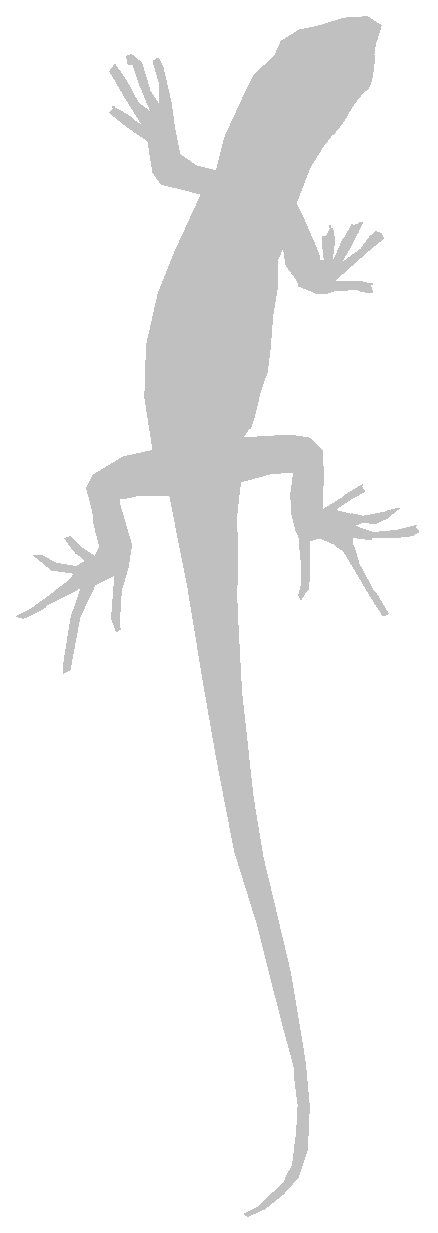
\includegraphics[width=0.1\textwidth,angle=270]{../../_common/fig/logo.eps}
\end{center}

\cleardoublepage

\vspace*{12cm}
\begin{tabular}{ll}
Author      & David Kneis \\
Affiliation & Institute of Earth and Environmental Sciences \\
            & Hydrology \& Climatology Section, \\
            & University of Potsdam, Germany \\
Contact     & david.kneis [at] uni-potsdam.de \\
            & \\
Project     & PROGRESS \\
Sub-project & D2.2 \\
Funding     & German Ministry of Education and Research (BMBF) \\
            & \\
Last update & \today{} \\
\end{tabular}

\vspace*{2.0cm}
\noindent Please help to improve this document by sending suggestions, corrections, wishes, and other useful feedback to the author (see above).

\cleardoublepage

%%%%%%%%%%%%%%%%%%%%%%%%%%%%%%%%%%%%%%%%%%%%%%%%%%%%%%%%%%
%%%%%%%%%%%%%%%%%%%%%% Page style   %%%%%%%%%%%%%%%%%%%%%%
%%%%%%%%%%%%%%%%%%%%%%%%%%%%%%%%%%%%%%%%%%%%%%%%%%%%%%%%%%

%%% Begin Fancy Header Settings
\pagestyle{fancy}                       % Sets fancy header and footer
\fancyfoot{}                            % Delete current footer settings
\renewcommand{\chaptermark}[1]{         % Lower Case Chapter marker style
  \markboth{\chaptername\ \thechapter\ \hspace{0.5cm} #1}{}}
\renewcommand{\sectionmark}[1]{         % Lower case Section marker style
  \markright{\thesection\ \hspace{0.5cm} #1}}
\fancyhead[LE,RO]{\bfseries\thepage}    % Page number (boldface) in left on even pages and right on odd pages
\fancyhead[RE]{\bfseries\leftmark}      % Chapter in the right on even pages
\fancyhead[LO]{\bfseries\rightmark}     % Section in the left on odd pages
\renewcommand{\headrulewidth}{0.3pt}    % Width of head rule %%% Clear Header
%% End Fancy Header Settings

%%%%%%%%%%%%%%%%%%%%%%%%%%%%%%%%%%%%%%%%%%%%%%%%%%%%%%%%%%
%%%%%%%%%%%%%%%%%%%%%% TOC          %%%%%%%%%%%%%%%%%%%%%%
%%%%%%%%%%%%%%%%%%%%%%%%%%%%%%%%%%%%%%%%%%%%%%%%%%%%%%%%%%

%% Begin TOC Settings
\pdfbookmark[1]{\contentsname}{toc}
\fancyhead[LE,RO]{\bfseries\thepage}
\fancyhead[RE]{\bfseries Contents}
\fancyhead[LO]{\bfseries Contents}
\tableofcontents
%% End TOC Settings

%%%%%%%%%%%%%%%%%%%%%%%%%%%%%%%%%%%%%%%%%%%%%%%%%%%%%%
%%%%%%%%%%%%%%%%%%%%%% ABSTACTS %%%%%%%%%%%%%%%%%%%%%%
%%%%%%%%%%%%%%%%%%%%%%%%%%%%%%%%%%%%%%%%%%%%%%%%%%%%%%

\onecolumn

% English summary
%\cleardoublepage
%\fancyhead[LE,RO]{\bfseries\thepage}
%\fancyhead[RE]{ }
%\fancyhead[LO]{ }
%\selectlanguage{american}
%\section*{Abstract}
\addcontentsline{toc}{chapter}{Abstract}

English abstract.



% German dummary
%\cleardoublepage
%\fancyhead[LE,RO]{\bfseries\thepage}
%\fancyhead[RE]{ }
%\fancyhead[LO]{ }
%\selectlanguage{ngerman}
%\section*{Kurzfassung}
\addcontentsline{toc}{chapter}{German abstract}

Deutsches Abstract.


%\selectlanguage{american}
%\cleardoublepage

%%%%%%%%%%%%%%%%%%%%%%%%%%%%%%%%%%%%%%%%%%%%%%%%%%%%%%%%%%
%%%%%%%%%%%%%%%%%%%%%% THE CHAPTERS %%%%%%%%%%%%%%%%%%%%%%
%%%%%%%%%%%%%%%%%%%%%%%%%%%%%%%%%%%%%%%%%%%%%%%%%%%%%%%%%%

\twocolumn

% Reestablish header
\fancyhead[LE,RO]{\bfseries\thepage}    % Page number (boldface) in left on even pages and right on odd pages
\fancyhead[RE]{\bfseries\leftmark}      % Chapter in the right on even pages
\fancyhead[LO]{\bfseries\rightmark}     % Section in the left on odd pages

%%%%% Chapter sources

\chapter{Catchment modeling utilities (R-package \software{topocatch})} \label{chap:topocatch}
\renewcommand{\tabdir}{chapters/topocatch/tab}
\renewcommand{\figdir}{chapters/topocatch/fig}

%%%%%%%%%%%%%%%%%%%%%%%%%%%%%%%%%%%%%%%%%%%%%%%%%%%%%%%%%%%%%%%%%%%%%%%%%%%%%%%%
%%%%%%%%%%%%%%%%%%%%%%%%%%%%%%%%%%%%%%%%%%%%%%%%%%%%%%%%%%%%%%%%%%%%%%%%%%%%%%%%
%%%%%%%%%%%%%%%%%%%%%%%%%%%%%%%%%%%%%%%%%%%%%%%%%%%%%%%%%%%%%%%%%%%%%%%%%%%%%%%%
\section{Purpose} \label{sec:topocatch:purpose}

The purpose of \software{topocatch} \citep{topocatch} is to extract and pre-process information required by semi-distributed rainfall-runoff models from spatial data. This includes, for example
\begin{itemize}
  \item the identification of (sub)-catchments.
  \item the determination of basic attributes of sub-catchments and river reaches.
  \item the analysis of input-output relation between the modeled objects (catchments, reaches, nodes, etc.).
  \item the estimation of river-cross section properties for sites where no survey data are available.
\end{itemize}

\software{topocatch} is distinguished from similar pre-processors by the following attributes:

\paragraph{Non-interactive} Once a suitable R-script is written, the pre-processing runs without user interaction. Thus, whenever the spatial input data changes due to updates, corrections, or modifications, \emph{all} steps of processing can be repeated without any effort.

\paragraph{Optional river net generation} Pre-processors for hydrological models typically generate a river net from the digital elevation model (DEM). This option is also available in \software{topocatch}. As an alternative, however, the user can supply an existing river net file. Such a file may originate, for example, from digitized topographic maps, field surveys or it could be a DEM-derived river net including manual adjustments. Supplying an external (or manually modified) river net file results in great flexibility. Some advantages are:
\begin{itemize}
  \item It can be achieved that the computed sub-catchments closely correspond to their natural counterparts.
  \item The user has the chance to split long reaches into several shorter segments and, hereby, gets control over both the minimum \emph{and maximum} size of sub-catchments.
  \item Special features (such as reservoirs, canals, or pipes) may be integrated into the river net file and considered in the processing.
\end{itemize}

\paragraph{Created output} The produced outputs are mostly in a format which can readily be used as input to rainfall-runoff models built with the \software{echse} simulation environment \citep[see][]{Echse-Main-Doc}.

Until 2012, \software{topocatch} used to be single, self-contained R-script whose behavior was controlled by a large number of configuration options. In 2013, \software{topocatch} was converted into a regular R-package to facilitate software maintenance, distribution, and documentation. Therefore, \software{topocatch} is no longer a single, ready-to-use script. Instead, the user has to write his/her own R-script that combines the various methods supplied by the package in a reasonable way. Some guidelines are provided in subsequent sections. Refer to the package's documentation for details on the various methods.

%%%%%%%%%%%%%%%%%%%%%%%%%%%%%%%%%%%%%%%%%%%%%%%%%%%%%%%%%%%%%%%%%%%%%%%%%%%%%%%%
%%%%%%%%%%%%%%%%%%%%%%%%%%%%%%%%%%%%%%%%%%%%%%%%%%%%%%%%%%%%%%%%%%%%%%%%%%%%%%%%
%%%%%%%%%%%%%%%%%%%%%%%%%%%%%%%%%%%%%%%%%%%%%%%%%%%%%%%%%%%%%%%%%%%%%%%%%%%%%%%%

%%%%%%%%%%%%%%%%%%%%%%%%%%%%%%%%%%%%%%%%%%%%%%%%%%%%%%%%%%%%%%%%%%%%%%%%%%%%%%%%
\section{Installation} \label{sec:topocatch-install}

In order to use the \software{topocatch}, the \software{R} software for statistical computing is required. See \citet{Echse-Install-Doc} for information on how to obtain and install this software.

The \software{topocatch} package is distributed as a tarball archive. See the respective section in \citet{Echse-Install-Doc} for more information on how to install such add-on packages on your system. Note that \software{topocatch} internally uses Fortran source code. Thus, a Fortran compiler must be available on the system in order to successfully build the package. The recommended compiler is GNU \software{gfortran}.

Currently, \software{topocatch} depends on the following additional R-packages: \software{shapefiles}, \software{maptools}, and \software{foreign}. These packages need to be installed prior to \software{topocatch}.

%%%%%%%%%%%%%%%%%%%%%%%%%%%%%%%%%%%%%%%%%%%%%%%%%%%%%%%%%%%%%%%%%%%%%%%%%%%%%%%%
%%%%%%%%%%%%%%%%%%%%%%%%%%%%%%%%%%%%%%%%%%%%%%%%%%%%%%%%%%%%%%%%%%%%%%%%%%%%%%%%
%%%%%%%%%%%%%%%%%%%%%%%%%%%%%%%%%%%%%%%%%%%%%%%%%%%%%%%%%%%%%%%%%%%%%%%%%%%%%%%%
\section{Standard documentation} \label{sec:topocatch:docs}

After the \software{topocatch} package has been loaded with the R command

\begin{lstlisting}[style=R]
library("topocatch")
\end{lstlisting}

a list of all provided methods can be generated with

\begin{lstlisting}[style=R]
help(package="topocatch")
\end{lstlisting}

The documentation of the individual methods can be displayed by typing the question mark followed by the name of the method, for example

\begin{lstlisting}[style=R]
?hydroModelData
\end{lstlisting}

Those who consider to use this package for the first time probably want to read the following sections to get a better understanding of the general concepts and the purpose of the various methods.

%%%%%%%%%%%%%%%%%%%%%%%%%%%%%%%%%%%%%%%%%%%%%%%%%%%%%%%%%%%%%%%%%%%%%%%%%%%%%%%%
%%%%%%%%%%%%%%%%%%%%%%%%%%%%%%%%%%%%%%%%%%%%%%%%%%%%%%%%%%%%%%%%%%%%%%%%%%%%%%%%
%%%%%%%%%%%%%%%%%%%%%%%%%%%%%%%%%%%%%%%%%%%%%%%%%%%%%%%%%%%%%%%%%%%%%%%%%%%%%%%%

\section{Supported data file formats} \label{sec:topocatch:formats}

\subsection{Overview} \label{sec:topocatch:formats-overview}

A typical pre-processing script for hydrological modeling using \software{topocatch} uses the following spatial data sets as input (see \figref{fig:topocatch-inputdata}):

\begin{description}
  \item [A digital elevation model (DEM) as a grid] The grid values can be either integers or floating point numbers.
  \item [One or more soil maps as grid(s)] The grid values can be integers (\eg{} encoding the soil types) or quantitative properties such as conductivities, for example.
  \item [A map of land use] The grid values are usually integers encoding the land use classes.
  \item [An optional vector file representing the river net] Must be a shape file containing line features (sometimes called arcs). The attribute table must have (at least) one field with feature IDs (of integer type) and a class field (of type string). See \secref{sec:topocatch:hints-shape} on practical issues and restrictions related to the creation of this file. If this input is not available, \software{topocatch} provides a method to generate an appropriate vector file from the DEM.
\end{description}

Thus, we deal with both raster and vector data.

\begin{figure}
  \centering
  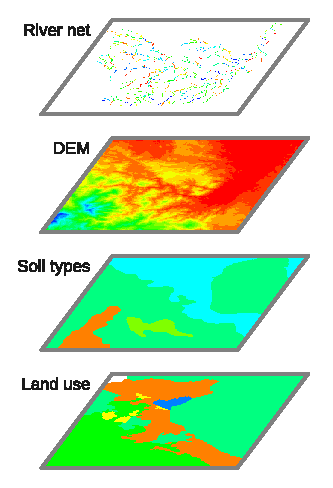
\includegraphics[width=0.75\columnwidth]{\figdir/inputdata.eps}
  \caption{The four spatial input data sets of \software{topocatch}. \label{fig:topocatch-inputdata}}
\end{figure}

\subsection{ASCII grid format} \label{sec:topocatch:formats-grid}

All input raster data, \eg{} those mentioned in \secref{sec:topocatch:formats-overview}, used by \software{topocatch} must be ASCII grids. This is a widely used exchange format for spatial raster data. It was originally used by ESRI's GIS systems but can be imported and exported by many other GIS, including free software such as QGIS.

A file in ASCII grid format is a plain text file (\figref{fig:asciigrid}). The first six lines of the file contain header information and the remaining lines hold the actual grid data as a matrix (one row per line). The meaning of the keywords in the header in as follows:

\begin{description}
  \item [ncols] Number of columns in the matrix of values starting at line 7 of the file.
  \item [nrows] Number of rows in the matrix of values starting at line 7 of the file.
  \item [xllcorner] X-coordinate corresponding to the lower left corner of the cell in the lower left corner of the matrix. Defines the Western border of the grid.
  \item [yllcorner] Y-coordinate corresponding to the lower left corner of the cell in the lower left corner of the matrix. Defines the Southern border of the grid.
  \item [cellsize] Length of a grid cell's edge. This is a single value, i.e.{} cells are quadratic.
  \item [NODATA\_value] Numerical value used to identify missing (or invalid) data in the values matrix.
\end{description}

\begin{figure}
  \lstinputlisting[style=txt]{\figdir/asciigrid.asc}
  \caption{Example of a file in ASCII grid format. \label{fig:asciigrid}}
\end{figure}

\subsection{Shape file format} \label{sec:topocatch:formats-vector}

This vector geo-data format can be im- and exported by most GIS systems including ESRI's GIS software, and QGIS, for example. It can be imported and exported by R as well. A shape file consists of (at least) three separate files with an identical basename and the extensions \texttt{.shp}, \texttt{.shx}, and \texttt{.dbf}. These are binary files containg coordinates, indices, and attribute data, respectively.

%%%%%%%%%%%%%%%%%%%%%%%%%%%%%%%%%%%%%%%%%%%%%%%%%%%%%%%%%%%%%%%%%%%%%%%%%%%%%%%%
%%%%%%%%%%%%%%%%%%%%%%%%%%%%%%%%%%%%%%%%%%%%%%%%%%%%%%%%%%%%%%%%%%%%%%%%%%%%%%%%
%%%%%%%%%%%%%%%%%%%%%%%%%%%%%%%%%%%%%%%%%%%%%%%%%%%%%%%%%%%%%%%%%%%%%%%%%%%%%%%%
\section{Typical usage} \label{sec:topocatch:usage}

The methods provided by the \software{topocatch} package can be combined in various ways. The subsequent sections describe a typical case of usage based on the most important high-level routines.

%%%%%%%%%%%%%%%%%%%%%%%%%%%%%%%%%%%%%%%%%%%%%%%%%%%%%%%%%%%%%%%%%%%%%%%%%%%%%%%%
\subsection{Step 1: Filling of the elevation model (\function{dem.fill})}
Most digital elevation models (DEM) contain sinks. They represent either natural or man-made depressions in the earth surface or artifacts of remote sensing. The filling of such sinks is a necessary step because their existence would hinder the identification of continuous drainage paths. In contrast to other software tools, the designated method in \software{topocatch} uses a non-iterative approach to fill the sinks. Its method's name is \function{dem.fill}. See the package's internal documentation for details on the method's arguments.

For large elevation models, the filling of sinks may consume a considerable amout of computation time. Therefore, it may be favourable to apply \function{dem.fill} once and to save its output for later re-use. This is highly if the entire pre-processing script is still under development.

%%%%%%%%%%%%%%%%%%%%%%%%%%%%%%%%%%%%%%%%%%%%%%%%%%%%%%%%%%%%%%%%%%%%%%%%%%%%%%%%
\subsection{Step 2: Analysis of the filled elevation model (\function{dem.analyze})}
The method \function{dem.analyze} is used to analyze the sink-filled elevation model. It computes flow direction codes, the flow accumulation, the concentration time index and it finally generates a vector file of the flow paths. See the package's internal documentation for details on the method's arguments. Some details on internal algorithms are given below.

\subsubsection*{Identification of flow directions}
The flow direction is computed for each cell of the DEM. It is identical to the direction of the steepest downward gradient (single-direction approach). The used algorithm is capable of handling locally flat areas. The result is an integer grid with values in the range 1$\ldots$8. The meaning of these codes is shown in \figref{fig:flowdirection-codes}.

\begin{figure}
  \centering
  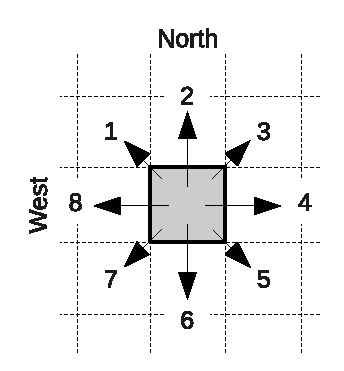
\includegraphics[width=0.5\columnwidth]{\figdir/flowdirection-codes.eps}
  \caption{Flow directions encoded as integer values. \label{fig:flowdirection-codes}}
\end{figure}

\subsubsection*{Calculation of flow accumulation}
For each cell of the DEM, the flow accumulation is computed as the number of upstream cells. This information is obtained from the grid of flow direction codes.

\subsubsection*{Calculation of concentration time indexes}
A concentration time index $cti$ is computed for each raster cell. The $cti$ is derived from the definition of the flow velocity $u$ according to \eqnref{eqn:topocatch:velocity} and Manning's equation (\eqnref{eqn:topocatch:manning}).

\begin{align}
  u= & \frac{L}{T} \label{eqn:topocatch:velocity} \\
  u= & \frac{1}{n} \cdot \sqrt{S_0} \cdot R^{2/3} \label{eqn:topocatch:manning}
\end{align}

In \eqnref{eqn:topocatch:velocity}, $L$ is the length of the flow path and $T$ is the corresponding travel time. In \eqnref{eqn:topocatch:manning}, $n$ represents the roughness (known as Manning's n), $S_0$ is the energy slope, and $R$ is the hydraulic radius. For steady flow problems, $S_0$ is equivalent to the surface slope. For small flow depths (in particular for overland flow), $R$ is dominated by the flow width and the flow depth has little influence. Merging \eqnsref{eqn:topocatch:velocity} \& \ref{eqn:topocatch:manning} into a single expression and solving for the travel time $T$ yields \eqnref{eqn:topocatch:traveltime}.

\begin{equation}
  T= \frac{L}{1/n \cdot \sqrt{S_0} \cdot R^{2/3}} \label{eqn:topocatch:traveltime}
\end{equation}

The $cti$ is finally derived from \eqnref{eqn:topocatch:traveltime} by simply neglecting the linear terms $1/n$ and $R^{2/3}$. This is equivalent to treating $n/R^{2/3}$ as a scaling constant for which a value of 1 is assumed. Then, the $cti$ for a particular cell $k$ of the elevation model can be calculated with \eqnref{eqn:topocatch:cti}.

\begin{equation}
  cti(k)= \sum_{i=1}^{nk}{\frac{L_i}{\sqrt{dz_i / L_i}}} \label{eqn:topocatch:cti}
\end{equation}

In this equation, $nk$ represents the number of raster cells through which the runoff generated in cell $k$ must flow until it is discharged into a river. $L_i$ is the (horizontal) length of path segment $i$. If the flow direction code of cell $i$ is 2, 4, 6, or 8 (see \figref{fig:flowdirection-codes}), $L_i$ is equivalent to the width of a raster cell. If the flow direction code is an odd number, $L_i$ is the width of a cell multiplied by $\sqrt{2}$. Furthermore, $dz_i$ is the elevation difference between cell $i$ and the neighboring cell into which cell $i$ drains. The user must specify a lower limit for $dz_i$ to avoid zero division in cases where a flow path crosses a flat area.

In the resulting grid, the $cti$ value of a cell will be larger, the longer the flow path and the lower the surface slope along the flow path is. Small $cti$ values are found for near-river cells and where steep surface slopes occur. Later in the processing, characteristic values (such as a mean $cti$) are computed for the individual catchments. These values may be used as indicators for the rate of runoff concentration in the individual catchments, since they integrate information on the catchment's shape, drainage density, and slope. The indicators primarily reflect the \emph{differences} between the catchments in terms of runoff concentration. To estimate actual concentration times, the $cti$ values need to be multiplied by appropriate calibration parameters (recall the derivation of \eqnref{eqn:topocatch:cti} from \eqnref{eqn:topocatch:traveltime}).

\subsubsection*{Generation of drainage lines (river net)}
The \function{dem.analyze} method finally generates a shape file representing the drainage lines, \ie{}rivers, based on the computed flow direction codes. Since the elevation model is the only source of information used, the result may differ from reality. This is especially true where the drainage network was altered by human action (canals, reservoirs, river training, etc.).

%%%%%%%%%%%%%%%%%%%%%%%%%%%%%%%%%%%%%%%%%%%%%%%%%%%%%%%%%%%%%%%%%%%%%%%%%%%%%%%%
\subsection{Step 3: Identification of model objects (\function{hydroModelData})}
After the DEM has been pre-processed and analyzed by \function{dem.fill} and \function{dem.analyze}, the major objects used in hydrological modeling (sub-basins, river reaches, etc.) need to be identified. This is achieved by a call to the high-level method \function{hydroModelData}. See the package's internal documentation for details on the method's arguments. Some background on the internal algorithms is provided below.

\subsubsection*{Vector-to-raster conversion of drainage lines}
For the identification of sub-basins, the drainage lines must be converted to a grid. 
The drainage lines must be provided as a shape file which can be created in the following ways:
\begin{itemize}
  \item It can be generated by \function{dem.analyze} which is the usual option for catchments without human alteration of the drainage system.
  \item It can an output of \function{dem.analyze} with subsequent manual modifications. Such modifications are typically required to take special objects like reservoirs, for example, into account.
  \item The shape file can be a digitized version of the basin's true river net. In this way it can be achieved that the generated sub-basins correspond to the actual river net as close as possible.
\end{itemize}

The result grid is of type integer and has the same extent and resolution as the DEM. The value of grid cells touched by a particular line feature is set to the corresponding value of the shape file's ID field. A special 'nodata' value is assigned to all grid cells not touched by any line feature. Another special 'conflict' value is assigned to cells which are touched by several lines (with different IDs). After this step, a buffer (having the width of a certain number of cells) is created around the gridded lines (see \figref{fig:lines-to-grid}).

The result grid is used later to initialize the computation of catchments. Note that line features to which no catchment should be assigned are excluded from the vector-to-raster conversion. The IDs of those features, therefore, do not appear in the result grid. Whether a catchment is generated for a particular line feature is mainly controlled by the entry in the class field of the shape file's attribute table.

\begin{figure}
  \centering
  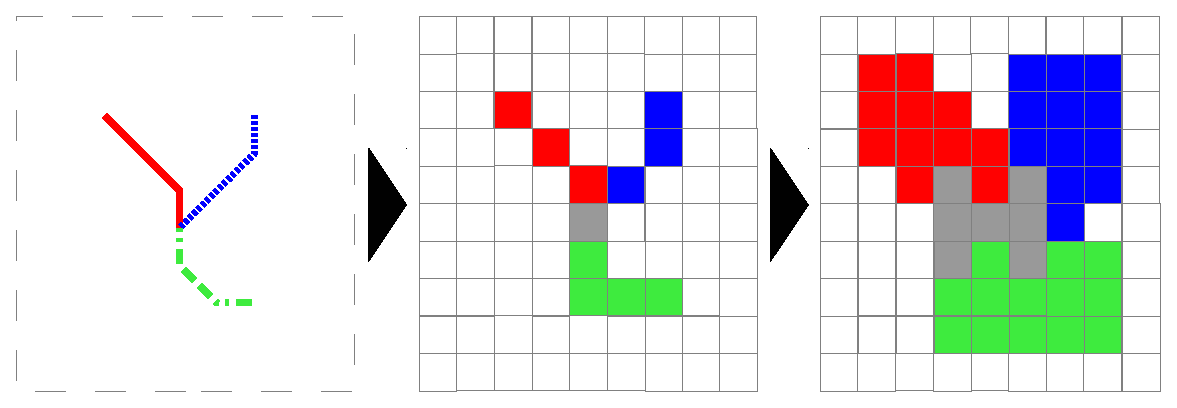
\includegraphics[width=0.95\columnwidth]{\figdir/lines-to-grid.eps}
  \caption[Steps of the vector-to-raster conversion.]{Steps of the vector-to-raster conversion. Left: Line features as vectors data. Middle: Gridded line features. Right: Gridded lines after buffering using a width of 1 cell. The 'nodata' value is indicated by white color, the 'confict' value by gray color. \label{fig:lines-to-grid}}
\end{figure}

\subsubsection*{Building of catchments}
The catchments are determined based on the grid of the flow directions and the grid of the rasterized lines (\figref{fig:lines-to-grid}). The latter grid is used as an initial estimate of the catchments where only near-river cells are set (to the ID of the corresponding reach). Starting from these reach cells (or near-reach cells if a buffer is used), the individual catchments 'grow' step-by-step by adding cells which discharge into the already set cells (according to the flow direction grid). The procedure continues until the catchments have reached their final size, \ie{} there are no more cells to add. The approach is illustrated in \figref{fig:build-catchments}.

\begin{figure}
  \centering
  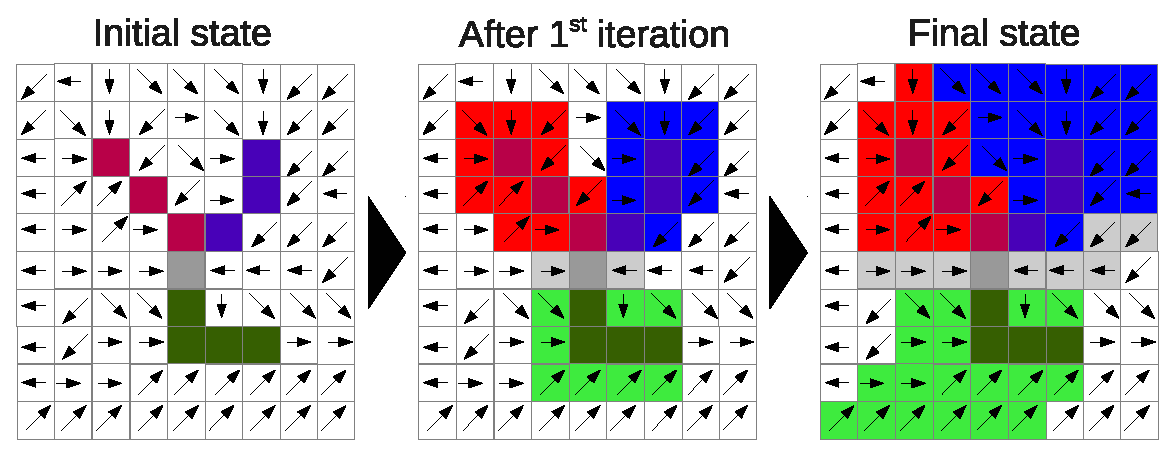
\includegraphics[width=0.95\columnwidth]{\figdir/build-catchments.eps}
  \caption[The approach used to iteratively build the catchments.]{The approach used to iteratively build the catchments. The dark-colored cells represent the initial cells carrying the ID of the corresponding reach (a buffer was omitted in this example). The arrows indicate the flow directions. In each iteration, new cells (in lighter colors) are added to the individual catchments. The gray-colored cell in the left grid has the special 'conflict' code because the junction of the reaches is located in that cell. A catchment is assigned to this cell too but the cells in this catchment carry a special 'conflict' value instead of a valid ID. These cells are reallocated (\ie{} added to the surrounding catchments) in a later step of processing. \label{fig:build-catchments}}
\end{figure}

As illustrated in \figref{fig:build-catchments}, cells discharging into a 'conflict' cell (\ie{} a cell that is in contact with multiple reaches), cannot be assigned to the catchment of a particular reach. Those cells are currently filled by a simple nearest neighbor interpolation.

\subsubsection*{Hydrological network assembly}
In this step, the linkage of the different objects (usually reaches and catchments) is analyzed and information on input-output-relations are dumped to tables. These tables can directly be used as an input for object-based hydrological catchment models built with the \software{echse} software.

The analysis of the network comprises a number of sub-steps, of which only the most important are mentioned below:

\begin{enumerate}
  \item The data in the shape file of the river network are checked for errors (non-unique IDs, missing attributes, etc.).
  \item The reach defining the systems outlet is identified.
  \item For each line feature contained in the shape file, the downstream neighbor is determined. In the usual case, this means that for each reach object, the connected downstream reach is identified.
  \item A catchment object is being linked to the line features (namely to all reach objects). Whether this actually happens for a particular line feature depends on the class of the feature (defined in the attribute table's class field) and further user-supplied settings.
  \item The upstream neighbor(s), if any, are identified for each line feature. If the number of upstream neighbors is greater than 1, an appropriate node object is inserted. The function of the node object is to collect the information (usually inflow data) from all upstream neighbors and to provide this information to the receiving downstream object.
  \item Several output tables are generated.
\end{enumerate}

Finally, basic attributes of the major objects are computed. For sub-basins, the location of the center of gravity and the drained area are calculated. For river reaches the computed properties include
\begin{itemize}
  \item the coordinates and elevation of end points,
  \item the reach length,
  \item the estimated bed slope,
  \item and the total area of upstream catchment.
\end{itemize}

As an optional step, the relation between the identified objects and stream gages can be identified. It is then known for each object whether a particular stream gage is affected by this object's output. Such information is helpful during the calibration of hydrological models. It also helps to spatially 'truncate' the model, \ie{} to restrict the model domain to the catchment of a specific stream gage.

%%%%%%%%%%%%%%%%%%%%%%%%%%%%%%%%%%%%%%%%%%%%%%%%%%%%%%%%%%%%%%%%%%%%%%%%%%%%%%%%
\subsection{Step 4: Calculation of additional sub-basin attributes}
Many hydrological catchment models require additional data in order to derive the sub-basin's parameters. Most typically, such information is obtained from digital maps of soil properties and land use. 

For the purpose of data extraction from such maps the \software{topocatch} package provides the two methods \function{geogrid.zones.continuous} and \function{geogrid.zones.classified}. Both methods require as input
\begin{enumerate}
  \item a primary grid with the computed sub-basins (defining the zones) and
  \item a second grid with the data to be analyzed for each zone.
\end{enumerate}

\subsubsection*{Extraction of continuous data}
The \function{geogrid.zones.continuous} method assumes that the second input grid contains data on a spatially continuous variable like elevation, for example. For each individual zone (\ie{} sub-basin) it calculates a statistics of that variable, namely the arithmetic mean, quantiles, and extremes with respect to the zone.

The method is typically used to determine for all sub-basins an average value and/or range of
\begin{itemize}
  \item elevation,
  \item a quantitative soil property (depth, hydraulic conductivity, etc.),
  \item the concentration time index returned by the \function{dem.analyze} method.
\end{itemize}

\subsubsection*{Extraction of classified data}
In contrast to that, the \function{geogrid.zones.classified} method assumes that the second input grid contains classified information such as land use codes (typically integers). For each individual zone (\ie{} sub-basin) it calculates the areal shares of all the classes.

The method is typically used to determine the areal fractions of land use classes for all sub-basins.

%%%%%%%%%%%%%%%%%%%%%%%%%%%%%%%%%%%%%%%%%%%%%%%%%%%%%%%%%%%%%%%%%%%%%%%%%%%%%%%%
\subsection{Step 5: Estimation of river cross-section properties} \label{sec:topocatch:xsregio}

\subsubsection*{Purpose}
Hydrological catchment models usually require river cross-section (x-section) information to be available for all modeled river reaches. This is because the propagation and attenuation of flood waves is controlled by the river's bed slope as well as the cross-section's conveyance (hydraulic radius, wet area, and roughness).

In real-world river basins, x-section survey data are usually available for a very limited number of reaches only. Consequently, x-section data for all other reaches being part of the model domain need to be estimated. If estimates cannot be gathered from the elevation model (see \secref{sec:topocatch:hints-xsExtract}), a spatial regionalization approach has to be adopted. The designated method in \software{topocatch} to perform this task is \function{xs.reachPars}. See R's internal help for detailed help on this methods's input arguments and outputs. Some additional background information is provided below.

\subsubsection*{Hydraulic properties of a single x-section}
According to Manning's equation (\eqnref{eqn:topocatch:xsregio:manning}), the \emph{steady} flow rate ($Q$) is controlled by four factors:
\begin{description}
  \item [$n$] The channel's roughness (friction and turbulence)
  \item [$S_0$] The slope of the channel.
  \item [$R$] The hydraulic radius.
  \item [$A$] The x-section's wet area.
\end{description}

\begin{align}
  Q= & \frac{1}{n} \cdot \sqrt{S_0} \cdot R^{2/3} \cdot A \label{eqn:topocatch:xsregio:manning}
\end{align}

\eqnref{eqn:topocatch:xsregio:manning} assumes that the x-section has a compact shape and, therefore, the channel's roughness can be described by a single value of $n$. In real x-sections, varying $n$ values may be appropriate to describe the different resistance of the main channel and the flood plain \citep[][]{Cunge1980}. However, the current version of \software{topocatch} is not capable of handling such so-called compound cross-sections and always assumes a unique $n$ value \footnote{Compound cross-sections may be analyzed with the software described in \chapref{chap:xsanalyzer}}. 

The two factors $A$ and $R$ in \eqnref{eqn:topocatch:xsregio:manning} are functions of the flow depth $D$ (see \figref{fig:topocatch:xsregio:xsection}). The shape of these functions is determined by the x-section's geometry. The steady flow rate $Q$ is a function of $D$ as well and $Q(D)$ represents the \emph{rating curve}. From \eqnref{eqn:topocatch:xsregio:manning} it is also obvious that there is a functional relation between $Q$ and $A$. Considering that the storage volume $V$ of a reach with length $L$ equals $A \cdot L$, there are also functional relations $Q(V)$ and $V(Q)$, respectvely.

\begin{figure}
  \centering
  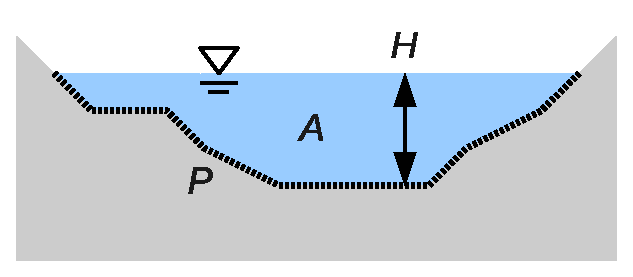
\includegraphics[width=0.95\columnwidth]{\figdir/xs_properties.eps}
  \caption[Definition of basic properties of a river cross-section.]{Definition of basic properties of a river cross-section ($D$: Flow depth, $A$: Wet area, $P$: Wet perimeter). The hydraulic radius is $R=A/P$. \label{fig:topocatch:xsregio:xsection}}
\end{figure}

In \software{topocatch}, it is assumed that, for an individual x-section, the characteristic functions $A(D)$ and $R(D)$ can be approximated by simple power functions as in \eqnref{eqn:topocatch:xsregio:xsfunction-A} \& \ref{eqn:topocatch:xsregio:xsfunction-R}. In these equations $a$, $b$, $c$, and $d$ are empirical coefficients to be identified by least-squares fitting.

\begin{align}
  A(H)= & a \cdot D ^b \label{eqn:topocatch:xsregio:xsfunction-A} \\
  R(H)= & c \cdot D ^d \label{eqn:topocatch:xsregio:xsfunction-R}
\end{align}

\subsubsection*{Cross-section estimation for arbitary sites}
For reaches where x-section information is not available, a multi-step estimation procedure is applied by \function{xs.reachPars}. It aims at estimating the functions \eqnsref{eqn:topocatch:xsregio:xsfunction-A} \& \ref{eqn:topocatch:xsregio:xsfunction-R} rather than the actual geometry data.

In the \textbf{first step}, two 'parent cross-sections' are identified from the pool of available survey data. These two cross-sections are selected in a way that
\begin{enumerate}
  \item the parent cross-sections are located as close as possible to the reach of interest, and
  \item the 1st cross-section has a smaller upstream catchment area and the 2nd one has a larger upstream catchment area than the reach of interest.
\end{enumerate}

This is illustrated in \figref{fig:topocatch:xsregio:regionalization_parentSelection}. Note that the two parent cross-sections are not necessarily located at the same branch of the river net.

\begin{figure}
  \centering
  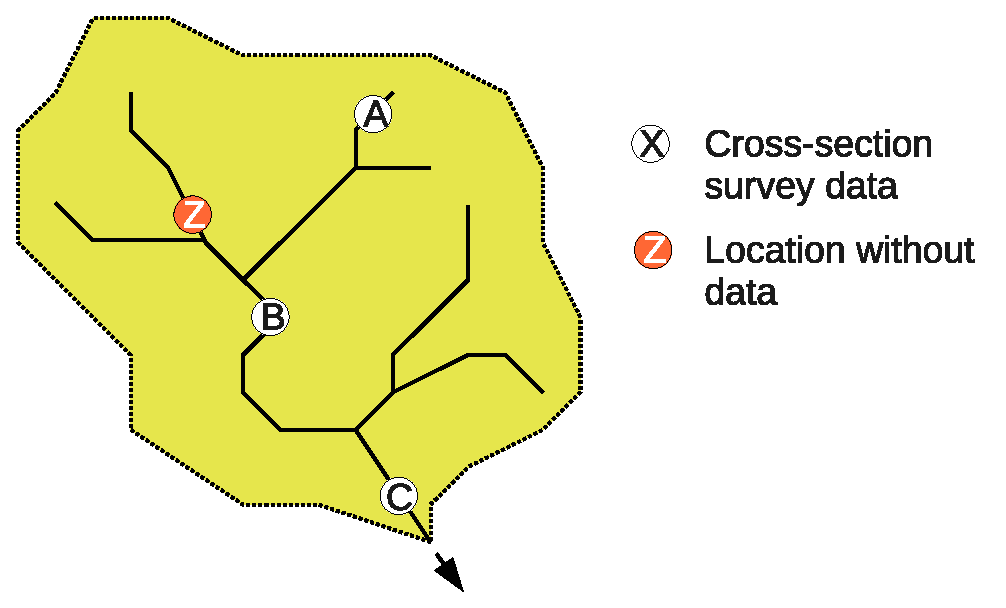
\includegraphics[width=0.95\columnwidth]{\figdir/xs_regionalization_parentSelection.eps}
  \caption[Selection of parent cross-sections for interpolation.]{Selection of parent cross-sections for interpolation. In the example, the data from A and B would be used to estimate the x-section's properties at location Z. \label{fig:topocatch:xsregio:regionalization_parentSelection}}
\end{figure}

In the \textbf{second step}, the characteristic functions $A(D)$ and $R(D)$ are computed for the two parent cross sections (solid graphs in \figref{fig:topocatch:xsregio:regionalization_interpolation}).

\begin{figure}
  \centering
  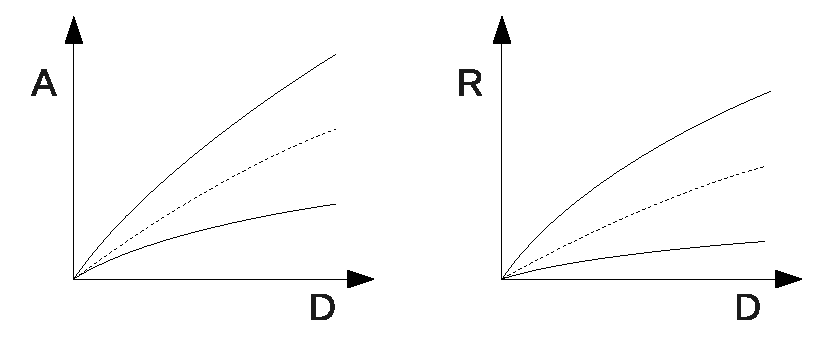
\includegraphics[width=0.95\columnwidth]{\figdir/xs_regionalization_interpolation.eps}
  \caption[Interpolation of the cross-section's characteristic functions.]{Interpolation of the cross-section's characteristic functions. Solid lines: Known relations for parent cross-sections. Dashed: Interpolated relation for a target location without survey geometry data. \label{fig:topocatch:xsregio:regionalization_interpolation}}
\end{figure}

Finally, in the \textbf{third step}, the characteristic functions $A(D)$ and $R(D)$ for the reach of interest are determined as a weighted average (dashed graphs in \figref{fig:topocatch:xsregio:regionalization_interpolation}). The applied weights are derived from the upstream catchment areas. If, for example, the upstream catchment area of the two parent cross-sections was 5 and 10 \sqkm{} and the reach of interest had an upstream catchment of 7 \sqkm{}, the information of the parent cross-sections would be weighted by $(7-5)/((7-5)+(10-7)) = 0.4$ and $(10-7)/((7-5)+(10-7)) = 0.6$, respectively. Note that, internally, the characteristic functions for all sites are approximated by power laws (\eqnsref{eqn:topocatch:xsregio:xsfunction-A} \& \ref{eqn:topocatch:xsregio:xsfunction-R}).

Once the functions $A(D)$ and $R(D)$ have been estimated for the reach of interest, all other hydraulic properties can be derived using Manning's equation and known values for the bed slope, the roughness, and the reach length.

It has to be noted that the above-mentioned approach of weighted averaging assumes that the x-sections's flow capacity (\ie{} the values of $A$ and $R$ for a given flow depth $D$) are (positively) correlated with the size of the upstream catchment. In many cases, this appears to be a reasonable assumption. However, the correlation may be weak (or not exist at all) if
\begin{itemize}
  \item the river basin's geology is heterogeneous, or
  \item a significant spatial gradient in rainfall is present.
\end{itemize}

In those cases, it may be better to sub-divide the river basin into zones of homogeneous geology/climate and to estimate the x-section characteristics separately for the zones.

It should also be noted that the assumed correlation between catchment size and flow capacity might not exist where cross-sections were constructed or altered by human action.

\subsubsection*{Example of the output}
An example output of the \function{xs.reachPars} method is shown in \figref{fig:topocatch:xsregio:output}. The data in that table can be used by hydrological models in various ways. Of special relevance are the values in the column dVdQ. They represent the derivative of the reach's storage volume with respect to the flow rate. This value (with the unit of a time) can be interepreted as the retention constant if the reach was treated as a (piece-wise) linear reservoir (\figref{fig:topocatch:xsregio:dVdQ}).

\begin{figure*}
\begin{lstlisting}[style=txt]
# Hydraulic properties of a reach for STEADY UNIFORM flow
#   Object ID:      '365'
#   Upstream area: 632.7
#   Reach length:  34485.996
#   Bottom slope:  0.000812
#   Roughness:     30
# 1st / 2nd parent cross-section:
#   IDs:       'xsEstim_in.extractedXS.xs5015.txt' / 'xsEstim_in.extractedXS.xs5037.txt'
#   weights:   0.998 / 0.00156
#   dist.s :   214865.7 / 195208.3
#   up. areas: 627.39 / 4023.72
# Descr. of columns:
#   Q:    Stream flow (L/T)
#   D:    Normal depth, i.e. max. flow depth (L)
#   A:    Wet x-section area (L^2)
#   V:    Storage volume (L^3)
#   dVdQ: Est. derivative dV/dQ (T)
Q	D	A	V	dVdQ
0	0	0	0	96814.34
1	0.15	4.489	154817.373	96814.34
2	0.21	7.297	251631.715	91503.91
5	0.327	13.871	478349.54	69669.92
10	0.457	22.546	777510.074	56102.11
20	0.639	36.651	1263931.218	45967.99
50	0.995	69.66	2402299.489	34986.86
100	1.392	113.237	3905080.393	28179.45
200	1.946	184.069	6347792.32	23084.84
500	3.031	349.858	12065191.465	17571.48
1000	4.238	568.699	19612163.977	14151.79
2000	5.925	924.423	31879638.649	11593.46
\end{lstlisting}
\caption{Example of an output file created by \function{xs.reachPars}. \label{fig:topocatch:xsregio:output}}
\end{figure*}

\begin{figure}
  \centering
  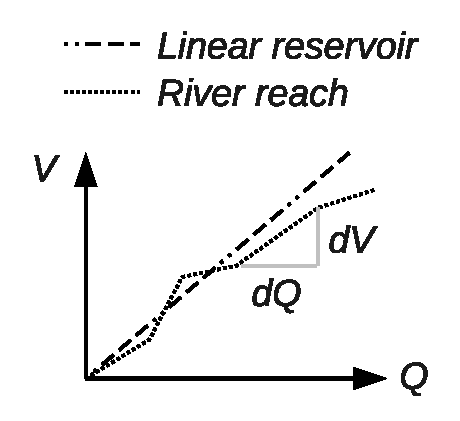
\includegraphics[width=0.5\columnwidth]{\figdir/xs_dVdQ.eps}
  \caption{Relation between the flow rate $Q$ and the storage volume $V$ for a linear reservoir and a river reach with an irregularly shaped cross-section. \label{fig:topocatch:xsregio:dVdQ}}
\end{figure}

%%%%%%%%%%%%%%%%%%%%%%%%%%%%%%%%%%%%%%%%%%%%%%%%%%%%%%%%%%%%%%%%%%%%%%%%%%%%%%%%
%%%%%%%%%%%%%%%%%%%%%%%%%%%%%%%%%%%%%%%%%%%%%%%%%%%%%%%%%%%%%%%%%%%%%%%%%%%%%%%%
%%%%%%%%%%%%%%%%%%%%%%%%%%%%%%%%%%%%%%%%%%%%%%%%%%%%%%%%%%%%%%%%%%%%%%%%%%%%%%%%
\section{Practical hints} \label{sec:topocatch:hints}

%%%%%%%%%%%%%%%%%%%%%%%%%%%%%%%%%%%%%%%%%%%%%%%%%%%%%%%%%%%%%%%%%%%%%%%%%%%%%%%%
\subsection{Processing of raster data} \label{sec:topocatch:hints-gridMethods}
In addition to the routines mentioned in \secref{sec:topocatch:usage}, the \software{topocatch} package provides many additional functions to facilitate the preparation of gridded spatial input data. For example:
\begin{itemize}
  \item \function{geogrid.readAscii}: Reads spatial grids in ASCII format.
  \item \function{geogrid.writeAscii}: Outputs spatial grids in ASCII format.
  \item \function{geogrid.reclass}: For classification of numeric values in a grid.
  \item \function{geogrid.fillGaps}: Replaces missing cell values based on a nearest neighbor search.
  \item \function{geogrid.valuesAtPoints}: Extracts data from a grid for specified locations.
  \item \function{xs.extractDEM}: Extracts cross-sections from an elevation model.   
\end{itemize}

See the R-package's built-in help for the full set of provided methods.

%%%%%%%%%%%%%%%%%%%%%%%%%%%%%%%%%%%%%%%%%%%%%%%%%%%%%%%%%%%%%%%%%%%%%%%%%%%%%%%%
\subsection{Making input grids consistent} \label{sec:topocatch:hints-gridConsistent}

Some of the methods contained in the \software{topocatch} package expect multiple grid as input arguments. This applies to the \function{geogrid.zones.continuous} and \function{geogrid.zones.classified} methods, for example. In those cases, the grids must cover (exactely) the same area with an identical resolution. In other words, the first 5 lines (see \figref{sec:topocatch:formats-grid}) of the corresponding ASCII grid files need to be identical. Since the data may come from different sources, a sequence of processing steps is typically required to make the grids spatially consistent. These steps are addressed in the subsequent paragraphs:

\paragraph{Resampling}
The first step is to make the cell size commensurate in all grids. This is typically known as resampling. For floating point grids like the DEM (bilinear) interpolation approaches are appropriate. When resampling integer grids (soil or land use data), one must use nearest neighbor methods, of course, in order not to introduce 'fractional' classes.

\paragraph{Clipping}
The second step is to clip the grids to an identical spatial window. The capabilities of clipping may be different in different GIS software. In QGIS 1.7.3, for example, one has to load the GDAL extension. With this extension loaded, a 'Clipper' functions is available in the menue 'Raster -- Extraction' which is capable of clipping grid data. The spatial target window of the clip operation can be defined either by another layer or directly by specifying the coordinates of the target window's limits. For the Marikina catchment (Philippines) for example, the following target window was used:

\begin{tabular}{lll} \hline\hline
  Limit   & Value & Defines border at \\
  \hline
  x1 & 289400 & West \\
  y1 & 1609000 & South \\
  x2 & 322200 & East \\
  y2 & 1641600 & North \\
  \hline
\end{tabular}

\paragraph{Conversion}
Once the grids have been clipped, they should be exported in ASCII grid format (see \secref{sec:topocatch:formats-grid}). Most GIS systems have this functionality. If this format is not supported, it may be possible to export the data in another matrix-based text format and then to manually add (or modify) the header (see \figref{fig:asciigrid}). A typically used file extension for ASCII grid files is \texttt{.asc} but this is not a true standard.

\paragraph{Final check}
Last but not least, the exported ASCII grid files should be opened in a (powerful) text editor and the first 5 lines of the header (see \secref{sec:topocatch:formats-grid}) need to be compared.

Although the same target window (or layer defining that window) was used in the clipping operation, it may happen that the header information are not exactely identical. This is due to the fact that the clipping simply removes cells outside the target window. It does, however, not apply a real spatial transformation to the data (which is more difficult) and, therefore, cannot correct for spatial shifts in x- or y-direction being smaller than the extend of a single cell.

A possible solution would be to apply a real spatial transformation prior to clipping of the grids. A more convenient workaround is to simply substitute the headers in all grids by the header of one 'master grid' (the DEM, for example). This approach works as long as the first two lines in the original grid headers are identical (i.e. the grids have the same number of rows and columns). The simple copy \& paste approach will introduce a spatial shift in two of the grids but the error should be less than the extent of a single cell. This will be tolerable in most situations (considering that a spatial transformation is an approximation as well).

After this step, the header information in the grids should be identical \emph{to the very last digit}, which is a prerequisite to run some of \software{topocatch}'s methods.

%%%%%%%%%%%%%%%%%%%%%%%%%%%%%%%%%%%%%%%%%%%%%%%%%%%%%%%%%%%%%%%%%%%%%%%%%%%%%%%%
\subsection{Creating a proper shape file} \label{sec:topocatch:hints-shape}

As mentioned in \secref{sec:topocatch:formats-overview}, a shape file of line features representing the river network is required as an input to the \function{hydroModelData} method. If this file is created manually rather than being generated by \software{topocatch}'s \function{dem.analyze} method, several aspects have to be considered related to both attributes and geometry.

\paragraph{Attributes}
The attribute table of the shape file must contain at least two fields: An ID field and a class field. The names of these fields can be chosen freely but recommended are 'id' and 'class', respectively.

The ID field must contain a \emph{unique} value that identifies each single feature in the shape file, \ie{} each single reach. The ID field should be of type integer.

The class field should be of string type. It allows to distinguish different classes of line features and to convey this information to \software{topocatch}. In a simple river system, a useful entry in the class field would be 'reach', for example, and this would be identical for all features. However, it would also be possible to include special features of a river network (such as reservoirs) in the shape file. For those features, a different class name (such as 'reservoir') would have to be entered in the class field.

\paragraph{Geometry and topology}
The conditions that must be fulfilled in terms of the features' geometry and topology are as follows:
\begin{description}
  \item [Single-part lines only] Some GIS systems support multi-part lines (line features with gaps in between). These must not appear in the shape file.
  \item [End-to-end connections] Line features must always be connected end-to-end. Thus, a line must not end at an intermediate vertex of another line. This also implies that junctions are always formed by 3 (or more) individual lines whose ends share the same coordinates. The alternative model where a side branch ends at some intermediate point of the main branch is not supported (see \figref{fig:shapefile-HowTo-junction} for an illustration).
  \item [Snapping] Where two line features have a connection, the coordinates of the connected end points need to be \emph{exactly} identical (to the very last digit). When digitizing the lines manually, this can \emph{only} be achieved by using the so-called snap functionality provided by all GIS systems.
  \item [No loops] The current version of \software{topocatch} only supports tree-like river systems. Thus, flow splits followed by junctions further downstream (\ie{} loops) must not exist in the river net.
  \item [Minimum length of reaches] As a rule of thumb, line features representing objects with a corresponding catchment -- namely reaches -- should not be shorter than about 4--5 times the cell size of the input grids. Thus, if the elevation model has a resolution of 100 m $\times$ 100 m, reaches should not be shorter than about 400--500 m. This is due to the fact that the shape file (vector data) is converted to a grid (raster data) within \software{topocatch}'s \function{hydroModelData} method and too short line features may get lost. Possible solutions for cases where the natural river system contains critically short reaches are discussed in \secref{sec:topocatch:hints-shortReach}. Note that line features to which no catchment should be assigned (which must be identified by an appropriate entry in the attribute table's class field) can be of arbitrary length.
  \item [Orientation of lines] The orientation of the individual line features is of no importance. Thus, it is OK to digitize lines in upstream or downstream directions and mixing both directions in the shape file is OK too.
\end{description}

\begin{figure}
  \centering
  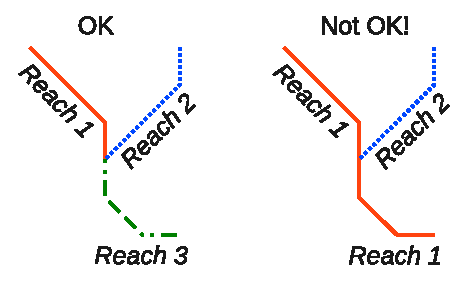
\includegraphics[width=0.6\columnwidth]{\figdir/shapefile-HowTo-junction.eps}
  \caption[Proper and improper junctions in a shape file.]{Left: Proper junction formed by three individual reaches (identified by different colors and styles). Right: Improper junction with a tributary ending in the mid-section of another reach. \label{fig:shapefile-HowTo-junction}}
\end{figure}

%%%%%%%%%%%%%%%%%%%%%%%%%%%%%%%%%%%%%%%%%%%%%%%%%%%%%%%%%%%%%%%%%%%%%%%%%%%%%%%%
\subsection{Handling very short reaches} \label{sec:topocatch:hints-shortReach}
In dense drainage networks, reaches may exist whose length is critically short (\figref{fig:shapefile-HowTo-shortReach}). Critical means that the length is less than about 4 times the resolution of the input grids (see \secref{sec:topocatch:hints-shape}). Those very short reaches may get lost during vector-to-raster conversion in the \function{hydroModelData} method and \software{topocatch} will generate an error because no catchment could be generated for some of the reaches contained in the shape file.

There are several possible solutions to this problem:
\begin{description}
  \item [Increasing the grid resolution] By resampling the elevation model (and all other input grids) to a finer resolution, the reach lengths increases relative to cell size. Consequently, there is a higher chance that even short reaches are retained in the vector-to-raster conversion. The drawback of this approach is, however, that the input grids become much larger and the computation becomes slower. For example, reducing the cell size to 1/2 increases the number of values in the data matrix by a factor of 4.
  \item [Removal of the short reaches] An alternative would be to edit the shape file and remove the critically short reaches. In the example shown in \figref{fig:shapefile-HowTo-shortReach}, this would mean that the short dashed line is deleted and the junctions up- and downstream of that reach are merged into an artificial junction with three inflows. The drawback of this approach is that manual work is necessary. Also, the shape file does no longer represent the actual network. Finally, if a very large number of short reaches is deleted, this may also lead to a systematic error in travel times.
  \item [Increasing the reach length] The very short reaches could also be made longer manually in order to increase the probability of a successful vector-to-raster conversion. The disadvantages are similar to those related to the removal of the short reaches.
  \item [Using a separate class] Another option which is recommended in most cases is to declare the short reaches not as reach objects but as instances of a different class. An appropriate name for this class might be something like 'shortReach' or 'link'. This is simply achieved by changing the entry in the attribute table's class field for the critically short reaches to 'shortReach' or 'link', respectively. Most GIS systems provide a suitable tool to do this sort of table column calculations using expressions. One can then inform \software{topocatch}'s \function{hydroModelData} method that no catchments should be build for objects of that special class. This essentially solves the problem, because (like all features not having a catchment), the short reaches are excluded from the vector-to-raster conversion. As a consequence, however, the newly introduced class must also be declared and implemented in the rainfall-runoff model. This class could either provide the same functionality as the normal reach class or just have the functionality of a link (which simply copies its input to its output). If the shape file is generated by \software{topocatch} itself (\function{dem.analyze} method), one may specify a critical reach length to automatically assign a different class name to short reaches.
\end{description}

\begin{figure}
  \centering
  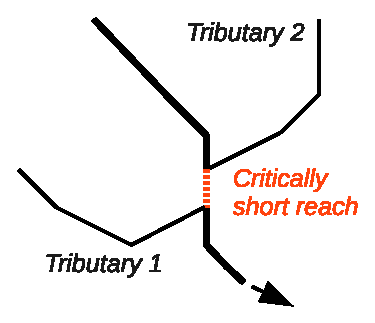
\includegraphics[width=0.5\columnwidth]{\figdir/shapefile-HowTo-shortReach.eps}
  \caption{Typical example of a critically short reach in a dense river network. \label{fig:shapefile-HowTo-shortReach}}
\end{figure}

%%%%%%%%%%%%%%%%%%%%%%%%%%%%%%%%%%%%%%%%%%%%%%%%%%%%%%%%%%%%%%%%%%%%%%%%%%%%%%%%
\subsection{Special features in the river net} \label{sec:topocatch:hints-specialFeatures}

As discussed earlier, the shape file may also contain other objects than river reaches. Such 'special' objects must
\begin{enumerate}
  \item be represented as lines, even if the objects are actually punctual (like gages or control structures, for example), or have an areal extent (reservoirs, lakes, etc.). This is due to the nature of the shape file format which restricts the contents to a single feature class (points \emph{or} lines \emph{or} polygons).
  \item be indicated by an appropriate entry in the attribute table's class field.
\end{enumerate}

Furthermore, if a catchment should be assigned to these objects (as in the case of lakes, for example), one needs to make \software{topocatch}'s \function{hydroModelData} method aware of this fact.

\subsubsection*{Example 1: A gage}
In a standard hydrological model, one would probably not treat gages as model objects. One would rather simply let the model output the flow rate of the reach to which the gage is attached. In operational models, however, is may be useful to treat gages as objects, because then, a gage may have some functionality. Typically, the observed flow would be defined as an external input variable of gage objects. In addition, some user-defined rule would be implemented that controls whether the simulated \emph{or} observed flow rates are submitted to the reach downstream of the gage.

In the shape file, a punctual gage object could be represented by a very short line feature (say of 1~m length). The resulting error in the system's total reach length would then be negligible.

\subsubsection*{Example 2: A reservoir}
Some more effort is necessary to include objects with an areal extent into the shape file of line features. This is demonstrated in \figref{fig:specialObjects-reservoir} with the example of a reservoir with two inflows. In situations like these, one must chose one line to represent the actual object. In the example, this is the line with ID 100. It is digitized in a zigzag manner to roughly cover the reservoir's surface area. This is done with the aim of increasing the chance that the reservoir's 'direct' catchment (\ie{} the area draining to the reservoir's shore line) is properly estimated from the elevation model.

To establish the original inter-connection, an artificial object with ID 101 is introduced. It is defined as an object of a separate class, here named 'link'. The functionality of this class is to simply transfer data. In the example, this link object redirects the outflow of reach 1 to a single inflow location for the reservoir without introducing a time lag.

\begin{figure}
  \centering
  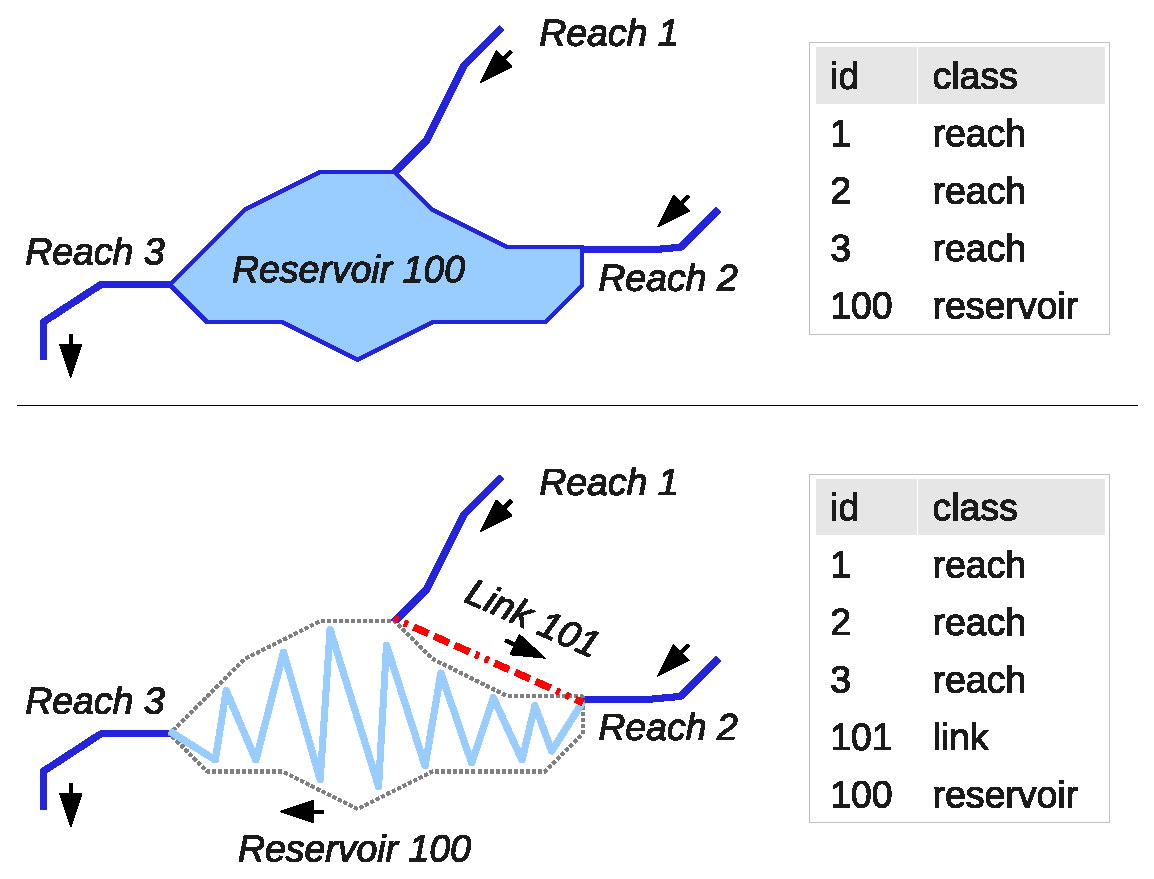
\includegraphics[width=0.95\columnwidth]{\figdir/specialObjects-reservoir.eps}
  \caption[Representation of a reservoir with two inflows in a map and in the input shape file.]{Representation of a reservoir with two inflows in a map (top) and in the input shape file (bottom). \label{fig:specialObjects-reservoir}}
\end{figure}

%%%%%%%%%%%%%%%%%%%%%%%%%%%%%%%%%%%%%%%%%%%%%%%%%%%%%%%%%%%%%%%%%%%%%%%%%%%%%%%%
\subsection{Extraction of river-cross sections from elevation models} \label{sec:topocatch:hints-xsExtract}

In \secref{sec:topocatch:xsregio} it was mentioned that data on river cross-section geometries are required for the set-up of many hydrological models. Since survey data are usually scarce, it may be desireable to extract such data from digital elevation models. For that purpose, the \software{topocatch} package provides a method \function{xs.extractDEM}. See the R-package documentation for more information.

%%%%%%%%%%%%%%%%%%%%%%%%%%%%%%%%%%%%%%%%%%%%%%%%%%%%%%%%%%%%%%%%%%%%%%%%%%%%%%%%
%%%%%%%%%%%%%%%%%%%%%%%%%%%%%%%%%%%%%%%%%%%%%%%%%%%%%%%%%%%%%%%%%%%%%%%%%%%%%%%%
%%%%%%%%%%%%%%%%%%%%%%%%%%%%%%%%%%%%%%%%%%%%%%%%%%%%%%%%%%%%%%%%%%%%%%%%%%%%%%%%
\section{TODO} \label{sec:topocatch:todo}

\subsection{HRU support} \label{sec:topocatch:todos-hru}
The current version of \software{topocatch} does \emph{not} generate the information needed by rainfall-runoff models using the hydrological reaction unit (HRU) approach. This is because of the fact that, so far, the \software{echse}-based hydrological models are intended to be used in operational forecasting. Such models typically need to be simpler than more process-oriented models for the sake of computational efficiency. However, it is not difficult to let \software{topocatch} generate input for HRU-based models and a future version might support this. \software{topocatch}'s source code would have to be adapted in two ways:
\begin{enumerate}
  \item Soil and land use information need to be merged into a single map prior to the calculation of areal shares with respect to the sub-basins using the \function{geogrid.zones.classified} method. This could be done, for example, by multiplying the soil code by a factor of 1000 and then adding the land use code. Then, the code of a HRU consisting of soil type 5 and land use type 12 would be 005012.
  \item In the \function{hydroModelData} method, an array of HRU-objects must be assigned to all reaches (and possibly further objects). At present, a single catchment object is assigned only.
\end{enumerate}



\chapter{R-package for model optimization (\software{mops})} \label{chap:mops}
\renewcommand{\tabdir}{chapters/mops/tab}
\renewcommand{\figdir}{chapters/mops/fig}

%%%%%%%%%%%%%%%%%%%%%%%%%%%%%%%%%%%%%%%%%%%%%%%%%%%%%%%%%%%%%%%%%%%%%%%%%%%%%%%%
%%%%%%%%%%%%%%%%%%%%%%%%%%%%%%%%%%%%%%%%%%%%%%%%%%%%%%%%%%%%%%%%%%%%%%%%%%%%%%%%
%%%%%%%%%%%%%%%%%%%%%%%%%%%%%%%%%%%%%%%%%%%%%%%%%%%%%%%%%%%%%%%%%%%%%%%%%%%%%%%%
\section{Purpose} \label{sec:mops:purpose}

The R-package \software{mops} provides a number of methods to facilitate the optimization of model parameters. The methods may be useful in the context of
\begin{itemize}
  \item model calibration.
  \item updating of operational models.
  \item optimization studies.
\end{itemize}

The methods provided in the \software{mops} package are designed for the following conditions:

\begin{itemize}
  \item The model, whose parameters are to be optimized, must be an executable file. In practice, this can be an executable built from source code (C++, FORTRAN, etc.) or a shell script. If it is a shell script, it typically calls an interpreter to process code written in a script language (R, Python, etc.).
  \item The executable must read the parameter values from plain text files. Thus, parameter values must \emph{not} be read from binary files or passed as command line arguments.
  \item The input parameters to be optimized must be floating point numbers. Internally, of course, the model can apply any kind of type conversion (typically to integer or logical).
  \item The text files holding the parameter values may be of arbitrary structure. However, the executable must read the numbers \emph{unformatted}. In other words, when reading a numeric value of one, for example, it must accept all of the following character representations \texttt{1}, \texttt{1.}, \texttt{1.0}, \texttt{1.0e+00}, \texttt{0.1e+01}. Note that legacy code sometimes uses \emph{formatted} read statements and may be incompatible with \software{mops}.
\end{itemize}

\software{echse}-based models generally comply with all of the conditions listed above.

%%%%%%%%%%%%%%%%%%%%%%%%%%%%%%%%%%%%%%%%%%%%%%%%%%%%%%%%%%%%%%%%%%%%%%%%%%%%%%%%
%%%%%%%%%%%%%%%%%%%%%%%%%%%%%%%%%%%%%%%%%%%%%%%%%%%%%%%%%%%%%%%%%%%%%%%%%%%%%%%%
%%%%%%%%%%%%%%%%%%%%%%%%%%%%%%%%%%%%%%%%%%%%%%%%%%%%%%%%%%%%%%%%%%%%%%%%%%%%%%%%
\section{Installation} \label{sec:mops:install}

The \software{mops} package is provided as a tarball. The package file name is \verb!mops_x.y.tar.gz! where x.y is a version number. See \citet{Echse-Install-Doc} for details on the installation procedure.

Note that the \software{mops} package depends on another R-package called \software{lhs} which allows for latin hypercube sampling. If the \software{lhs} package is not installed already, it needs to be downloaded and installed \emph{prior} to installing \software{mops}.

%%%%%%%%%%%%%%%%%%%%%%%%%%%%%%%%%%%%%%%%%%%%%%%%%%%%%%%%%%%%%%%%%%%%%%%%%%%%%%%%
%%%%%%%%%%%%%%%%%%%%%%%%%%%%%%%%%%%%%%%%%%%%%%%%%%%%%%%%%%%%%%%%%%%%%%%%%%%%%%%%
%%%%%%%%%%%%%%%%%%%%%%%%%%%%%%%%%%%%%%%%%%%%%%%%%%%%%%%%%%%%%%%%%%%%%%%%%%%%%%%%
\section{Standard documentation} \label{sec:mops:docs}

After the \software{mops} package has been loaded with the R command

\begin{lstlisting}[style=R]
library("mops")
\end{lstlisting}

a list of all provided methods can be generated with

\begin{lstlisting}[style=R]
help(package="mops")
\end{lstlisting}

The documentation of the individual methods can be displayed by typing the question mark followed by the name of the method, for example

\begin{lstlisting}[style=R]
?modelError_MCS
\end{lstlisting}

As always, the standard documentation for the methods is rather short. New users probably want to read the following sections to get a better understanding of the general concepts and the dependencies between the methods in the \software{mops} package.

%%%%%%%%%%%%%%%%%%%%%%%%%%%%%%%%%%%%%%%%%%%%%%%%%%%%%%%%%%%%%%%%%%%%%%%%%%%%%%%%
%%%%%%%%%%%%%%%%%%%%%%%%%%%%%%%%%%%%%%%%%%%%%%%%%%%%%%%%%%%%%%%%%%%%%%%%%%%%%%%%
%%%%%%%%%%%%%%%%%%%%%%%%%%%%%%%%%%%%%%%%%%%%%%%%%%%%%%%%%%%%%%%%%%%%%%%%%%%%%%%%
\section{Theoretical background} \label{sec:mops:background}

\subsection{Goal of optimization} \label{sec:mops:background:optimization:goal}

Optimization generally refers to the minimization\footnote{To solve a maximization problem, the objective function is simply multiplied by $-1$.} of the value of a function whose value depends on one or more parameters. This function is called the \emph{objective function}. Let's write the objective function as $f(p)$, with $f$ being the function's name and $p$ being a vector of parameters. In the special case of one-dimensional optimization, $p$ is simply a vector of length 1.

The goal of \emph{any} optimization procedure is to find a set of values for the parameters $p$ that minimizes the value of $f$.

\paragraph{Example 1 (minimization, 1-dimensional):} Determine the optimum dosage of a medicine for malaria protection that minimizes the total number of death from both infection and serious side effects ($f$: number of casualties, $p$: dosage).

\paragraph{Example 2 (maximization, 2-dimensional):} Determine the amounts of fertilizer and water to maximize the yield of a tomatoe field ($f$: yield, $p$: amounts of fertilizer and water).

\subsection{Optimization methods} \label{sec:mops:background:optimization:methods}

Depending on the nature of $f$ (non-linearities, discontinuities, local minima, etc.) and the number of unknown parameters in $p$, the optimization problem is more or less difficult to solve. Unfortunately, there is no general strategy that performs best in all cases. In fact, it is not even guaranteed that a $global$ minimum of $f$ is found at all.

One thing which is common to all optimization methods is that \emph{multiple} calls to $f$ for varying values of $p$ are necessary (bold arrow in \figref{fig:mops:concepts:optimization:multipleCalls_opt}). Only then, the effect of a change in the parameter value(s) $p$ on the value of $f$ can be detected.

\begin{figure}
  \centering
  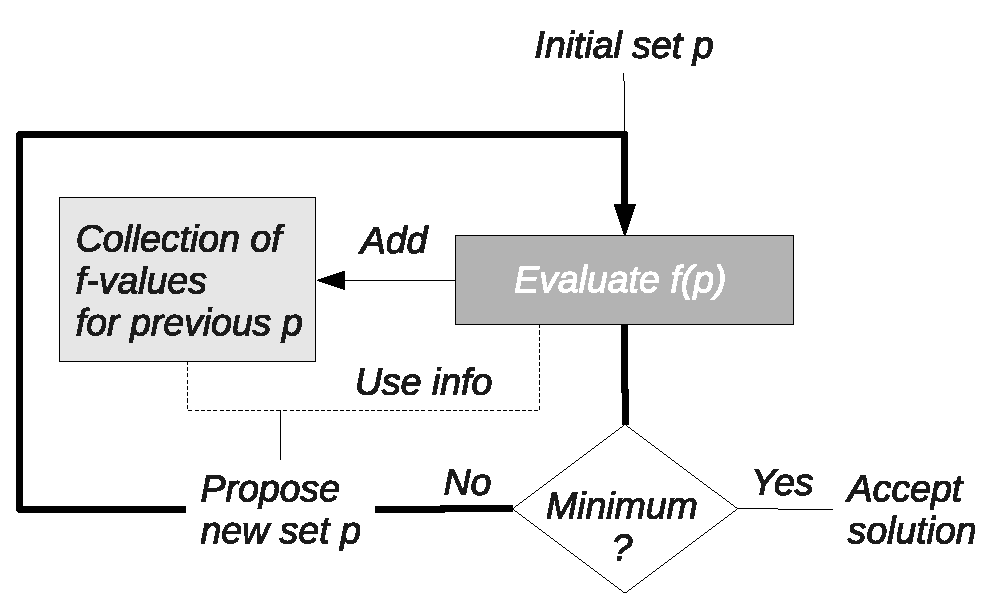
\includegraphics[width=0.9\columnwidth]{\figdir/multipleCalls_opt.eps}
  \caption{Basic outline of an optimization method. \label{fig:mops:concepts:optimization:multipleCalls_opt}}
\end{figure}

The basic strategies of optimization are distinguished by the way of how a new proposal for the values in $p$ is generated, given the information from the previous calls to $f$ for other values of $p$. The most important distinction is between \emph{deterministic} and \emph{stochastic} algorithms. Some examples and references for both types of strategies can be found in the help text of R's \texttt{optim} method.

As opposed to 'complete' optimization strategies, the technique of Monte-Carlo simulation does not identify a single optimum parameter set. Instead, the objective function is simply evaluated for a large number of random parameter sets (\figref{fig:mops:concepts:optimization:multipleCalls_mcs}). It is then up to a human to inspect the output and to draw conclusions on the suitability of parameter values.

\begin{figure}
  \centering
  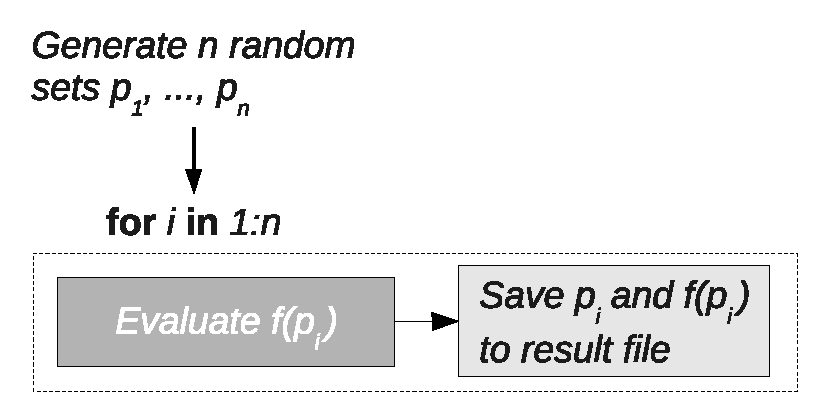
\includegraphics[width=0.7\columnwidth]{\figdir/multipleCalls_mcs.eps}
  \caption{Basic outline of Monte-Carlo simulation. \label{fig:mops:concepts:optimization:multipleCalls_mcs}}
\end{figure}

\subsection{Model error as objective function} \label{sec:mops:background:objFun}

In the context of a dynamic simulation, the objective function measures the deviation between a simulated time series (produced by the model) and a corresponding time series of observations. Generally, the deviation (synonyms: model error, performance, goodness-of-fit) depends on the values of the model's parameters. It may be helpful to see that this is very similar to the common case of fitting a linear model to a set of x,y-data (\figref{fig:mops:concepts:optimization:deviation}). The typical differences are:
\begin{itemize}
  \item In dynamic modeling, the x-axis represents the time.
  \item Real-world dynamic models often have more parameters than the linear model which has only 2 (slope and intercept).
  \item In many dynamic models, the relations between parameter values and the output are non-linear.
  \item In the case of dynamic simulation models, numerical methods are required to determine a set of optimum parameters (see \secref{sec:mops:background:optimization:methods}). For the linear model, an analytical expression exists to directly solve for slope and intercept.
\end{itemize}

\begin{figure}
  \centering
  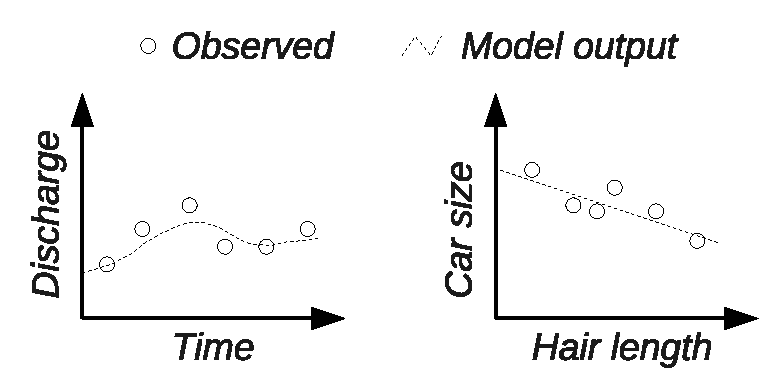
\includegraphics[width=0.9\columnwidth]{\figdir/deviation.eps}
  \caption{Goodness-of-fit for a dynamic simulation model (left) and an empirical linear model (right). \label{fig:mops:concepts:optimization:deviation}}
\end{figure}

The deviation between observations and the corresponding simulated values can be quantified by a variety of mathematical measures. In the case of linear fitting (\figref{fig:mops:concepts:optimization:deviation}, right), the sum of squared errors (SSE) is most often used. In dynamic modeling (\figref{fig:mops:concepts:optimization:deviation}, left), measures like the RMSE (root mean suared error) and the Nash-Sutcliffe index are usually preffered. They are based on the SSE as well but the values are more convenient to interpret.

In the context of dynamic modeling, the interior of a objective function $f(p)$ typically contains the steps listed in \tabref{tab:mops:background:objFun}.

\begin{table}
  \caption[Interior of an objective function in the context of dynamic modeling.]{Interior of an objective function in the context of dynamic modeling. It is assumed that the model reads all parameter values from text files. \label{tab:mops:background:objFun}}
  \begin{tabular}{p{0.03\columnwidth}p{0.85\columnwidth}} \hline\hline
  \# & Task \\ \hline
  1 & Get current parameter set $p$ (passed via the funcion's argument list). \\
  2 & Update the model's input files with the current values in $p$. \\
  3 & Run the model. \\
  4 & Read the model output (a time series). \\
  5 & Read observed data. \\
  6 & Compute the model error from the data read in steps 4 \& 5 using a suitable mathematical measure. \\
  7 & Return the result. \\ \hline\hline
  \end{tabular}
\end{table}

%%%%%%%%%%%%%%%%%%%%%%%%%%%%%%%%%%%%%%%%%%%%%%%%%%%%%%%%%%%%%%%%%%%%%%%%%%%%%%%%
\subsection{Semi-automatic calibration} \label{sec:mops:background:semiAutoCalib}

Environmental simulation models often have a large number of conceptual parameters whose values have to be calibrated based on observations. Without having a deeper understanding of the model's functioning, \ie{} the underlying equations, this is not a trivial task. Even if the equations are known, multi-dimensional, non-linear optimization remains a challenge and success is not guaranteed. The classic, deterministic optimization algorithms may fail for a number of reasons, such as truncation and round-off problems, insensitive parameters, complicated parameter interactions and compensations, non-continuous model behavior, or the existence of local minima. The alternative is the use of stochastic algorithms. Unfortunately, stochastic optimizers usually come with a number of algorithms parameters which affect convergence and computation times. If established general-purpose defaults do not exist, the estimation of these algorithm parameters is a problem on its own. Finally, a manual calibration by trial-and-error is often not practically feasible and the results have the reputation of being subjective.

Therefore, it is sometimes a good idea to fall back on the robust and straightforward concept of Monte-Carlo simulation (\figref{fig:mops:concepts:optimization:multipleCalls_mcs}). Some advantages of Monte-Carlo simulation are:
\begin{itemize}
  \item It simply cannot fail as long as the tested parameter sets do not cause invalid numeric results.
  \item There are no algorithm parameters.
  \item One can learn from the output about the (in)sensitivity of parameters, even if the model is a black box.
\end{itemize}

Especially useful is the concept of sequential Monte-Carlo simulation. This concept can be described by the following set of instructions:
\begin{description}
  \item[a)] Carry out a Monte-Carlo simulation with wide sampling ranges for all parameters.
  \item[b)] Visualize the results from step $a$. For each varied parameter, a scatter plot should be created with the parameter value on the x-axis and the model error on the y-axis.
  \item[c)] Inspect all plots created in step $b$. If a structure is visible in a plot, indicating an optimum range for the particular parameter, modify the sampling range of that parameter. Usually, the sampling range can be chosen narrower (unless the initial range was not wide enough).
  \item[d)] Return to step $a$, using the updated sampling range.
\end{description}

This semi-automatic approach to calibration has been successfully used in hydrological modeling \citep[see, \eg{}][]{Kneis2012}. It is certainly not among the most efficient strategies. However, the chance of complete failure is very low. Finally, with the above approach, it becomes visible whether the optimization problem is well behaved or of the nasty sort. Users of unsupervised optimization algorithms can only hope for a well behaved problem or guess on the cause of failure.

A practical example of parameter estimation using sequential Monte-Carlo simulation can be found in \secref{sec:mops:example_mcs:experiment}.

%%%%%%%%%%%%%%%%%%%%%%%%%%%%%%%%%%%%%%%%%%%%%%%%%%%%%%%%%%%%%%%%%%%%%%%%%%%%%%%%
%%%%%%%%%%%%%%%%%%%%%%%%%%%%%%%%%%%%%%%%%%%%%%%%%%%%%%%%%%%%%%%%%%%%%%%%%%%%%%%%
%%%%%%%%%%%%%%%%%%%%%%%%%%%%%%%%%%%%%%%%%%%%%%%%%%%%%%%%%%%%%%%%%%%%%%%%%%%%%%%%

\section{Important methods in \software{mops}} \label{sec:mops:methods}

\subsection{\function{update\_template}} \label{sec:mops:methods:update_template}

As illustrated in \figsref{fig:mops:concepts:optimization:multipleCalls_opt} and \ref{fig:mops:concepts:optimization:multipleCalls_mcs}, optimization methods and Monte-Carlo simulation involve many successive of evaluations of the objective functions for different parameter values. In each evaluation, the model's input files need to be updated (recall \tabref{tab:mops:background:objFun}). For this purpose, the \software{mops} package provides the \function{update\_template} method.

The method takes a template file and a \emph{named} vector of numerical values as input. It then scans the template file for the occurrence of \emph{placeholders}. A placeholder is a string enclosed by two designated characters, typically some sort of fancy brackets like \texttt{\{\}}, \texttt{[]} or \texttt{<>}. The \function{update\_template} method tries to replace every placeholder in the template file by the numerical value of a matching element from the input vector. A matching element is one whose name is identical to the placeholder's central string, \ie{} the string between the designated characters. The mode of action of the \function{update\_template} method is best demonstrated by the examples in \figsref{fig:mops:methods:update_template_example1} and \ref{fig:mops:methods:update_template_example2}.

\begin{figure}
  \centering
  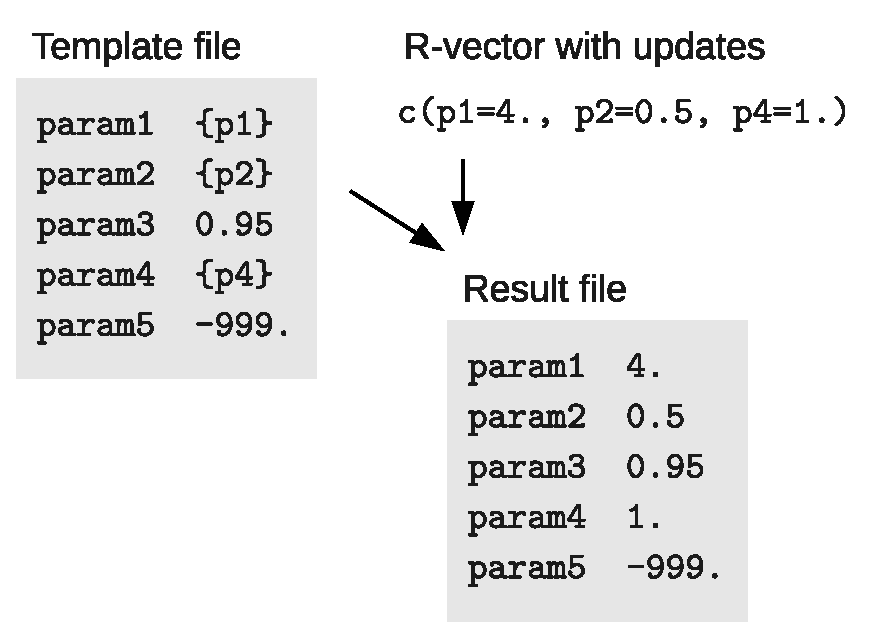
\includegraphics[width=0.7\columnwidth]{\figdir/update_template_example1.eps}
  \caption[Example application of the \texttt{update\_template} method.]{Example application of the \texttt{update\_template} method. Here, the characters to identify the start and the end of a placeholder are \texttt{``\{``} and \texttt{``\}``}, respectively. \label{fig:mops:methods:update_template_example1}}
\end{figure}

\begin{figure}
  \centering
  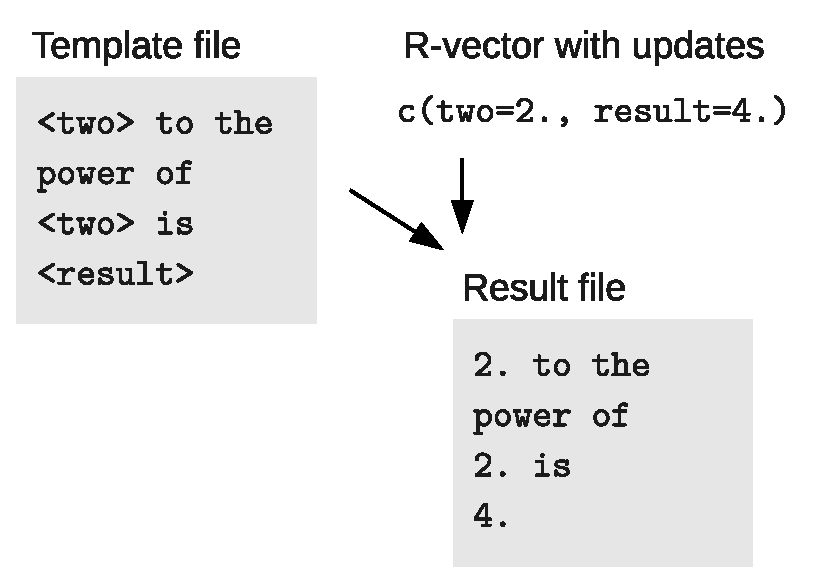
\includegraphics[width=0.7\columnwidth]{\figdir/update_template_example2.eps}
  \caption[Another example application of the \texttt{update\_template} method.]{Another example application of the \texttt{update\_template} method. Here, the characters to identify the start and the end of a placeholder are \texttt{``<``} and \texttt{``>``}, respectively. \label{fig:mops:methods:update_template_example2}}
\end{figure}

Although the \function{update\_template} can be called in isolation, it is mainly used as a sub-routine in other high-level methods of the \software{mops} package.

\subsection{\function{modelError\_multiDim}} \label{sec:mops:methods:modelError_multiDim}

The \function{modelError\_multiDim} is the central high-level method of the \software{mops} package. It represents a complete objective function. For a given parameter set, the method is able to perform all the steps listed in \tabref{tab:mops:background:objFun}. It can directly be used together with R's generic optimization method \texttt{optim}.

\subsection{\function{mcs\_run} and \function{mcs\_eval}} \label{sec:mops:methods:mcs}

The methods \function{mcs\_run} and \function{mcs\_eval} provide a complete framework for Monte-Carlo simulation. \function{mcs\_run} generates the random parameter sets and carries out all the simulations.  The function \function{mcs\_eval} calculates the corresponding model errors and creates graphics to summarize the results of Monte-Carlo experiments. A complete example for the use of these methods is provided in \secref{sec:mops:example_mcs}.

%%%%%%%%%%%%%%%%%%%%%%%%%%%%%%%%%%%%%%%%%%%%%%%%%%%%%%%%%%%%%%%%%%%%%%%%%%%%%%%%
%%%%%%%%%%%%%%%%%%%%%%%%%%%%%%%%%%%%%%%%%%%%%%%%%%%%%%%%%%%%%%%%%%%%%%%%%%%%%%%%
%%%%%%%%%%%%%%%%%%%%%%%%%%%%%%%%%%%%%%%%%%%%%%%%%%%%%%%%%%%%%%%%%%%%%%%%%%%%%%%%

\section{Example: Monte-Carlo simulation} \label{sec:mops:example_mcs}

%%%%%%%%%%%%%%%%%%%%%%%%%%%%%%%%%%%%%%%%%%%%%%%%%%%%%%%%%%%%%%%%%%%%%%%%%%%%%%%%
\subsection{Model equations} \label{sec:mops:example_mcs:modelEqn}

This section introduces the practical use of the \texttt{mcs\_run} method to perform a Monte-Carlo simulation. For the purpose of demonstration, we consider the fairly simple 1-dimensional advection-dispersion model (\eqnref{eqn:mops:example_mcs:modelEqn:ade-pde}). It describes the 1-dimensional (longitudinal) transport of dissolved, non-reactive matter in a river.

\begin{equation} \label{eqn:mops:example_mcs:modelEqn:ade-pde}
\dfrac{\partial c}{\partial t} = d \cdot \dfrac{\partial^2 c}{\partial x^2} - u \cdot \dfrac{\partial c}{\partial x}
\end{equation}

\begin{tabular}{lp{0.7\columnwidth}}
  $c$ & Concentration (g/m$^3$) \\
  $x$ & River station (m) \\
  $d$ & Dispersion coefficient in x-direction (m$^2$/s) \\
  $u$ & Average flow velocity in x-direction (m/s) \\
\end{tabular}

\medskip
This partial differential equation model has two parameters, $d$ and $u$. For certain conditions, \eqnref{eqn:mops:example_mcs:modelEqn:ade-pde} has the analytical solution presented in \eqnref{eqn:mops:example_mcs:modelEqn:ade-solution}.

\begin{equation} \label{eqn:mops:example_mcs:modelEqn:ade-solution}
  c(x,t)= \frac{m}{A \cdot \sqrt{4 \cdot \pi \cdot d \cdot t}} \cdot exp\left(\frac{-(x-u \cdot t)^2}{4 \cdot d \cdot t} \right)
\end{equation}

with the additional symbols

\begin{tabular}{lp{0.7\columnwidth}}
  $t$ & Time (s) \\
  $m$ & Mass (g) \\
  $A$ & Wet cross-section area (m$^2$) \\
\end{tabular}

\medskip
This solution assumes that
\begin{itemize}
  \item The injection of mass at $t=0$ occurs in an infinitesimally short time span.
  \item The mass is instantly distributed over the entire cross-section.
  \item The flow is steady (constant rate) and uniform (constant cross-section geometry).
\end{itemize}

The behavior of the model is illustrated in \figsref{fig:mops:example_mcs:modelEqn:fixedStations} and \ref{fig:mops:example_mcs:modelEqn:fixedTimes} for constant values of $m$=100, $a$=1, $d$=30, and $u$=0.5. \figref{fig:mops:example_mcs:modelEqn:fixedStations} shows the time series of concentration (chemographs) that one would obtain by frequent analysis of water samples taken at a particular river station. To get a picture as in \figref{fig:mops:example_mcs:modelEqn:fixedTimes}, one would have to organize synchronous sampling at multiple stations along the river.

\begin{figure}
  \centering
  \includegraphics[width=0.75\columnwidth]{\figdir/ad-equation_fixedStations.eps}
  \caption{Solutions of \eqnref{eqn:mops:example_mcs:modelEqn:ade-solution} at a fixed set of river stations for variable times. \label{fig:mops:example_mcs:modelEqn:fixedStations}}
\end{figure}

\begin{figure}
  \centering
  \includegraphics[width=0.75\columnwidth]{\figdir/ad-equation_fixedTimes.eps}
  \caption{Solutions of \eqnref{eqn:mops:example_mcs:modelEqn:ade-solution} at a fixed set of times for variable river stations. \label{fig:mops:example_mcs:modelEqn:fixedTimes}}
\end{figure}

%%%%%%%%%%%%%%%%%%%%%%%%%%%%%%%%%%%%%%%%%%%%%%%%%%%%%%%%%%%%%%%%%%%%%%%%%%%%%%%%
\subsection{Model implementation} \label{sec:mops:example_mcs:modelImpl}
The C++ source code listed in \figref{fig:mops:example_mcs:adModel_code} implements a simulation model based on the equations from \secref{sec:mops:example_mcs:modelEqn}. It solves \eqnref{eqn:mops:example_mcs:modelEqn:ade-solution} for a fixed station $x$ and an array of times. Thus, it computes a chemograph as in \figref{fig:mops:example_mcs:modelEqn:fixedStations}. For compatibility with the \software{mops} package, the executable reads all input data -- including the values of the two parameters $u$ and $d$ -- from a text file.

\begin{figure*}
  \lstinputlisting[style=c++]{\figdir/mcs_example/adModel.cpp}
  \caption{C++ source code of the advection-dispersion model (file: adModel.cpp). \label{fig:mops:example_mcs:adModel_code}}
\end{figure*}

To build an executable from the source code in \figref{fig:mops:example_mcs:adModel_code}, the GNU C++ compiler can be used \citep[see][for mode info]{Echse-Install-Doc}. Assuming that the source code is saved in a file 'adModel.cpp', an appropriate command line for compilation would be:

\begin{lstlisting}[style=shell]
  g++ -lstdc++ -o adModel adModel.cpp
\end{lstlisting}

The command should create an executable 'adModel' (possibly with an appropriate file name extension).

To successfully run the model, two command line arguments must be passed to the executable. The first argument is the name of the input file containing all input data, including the values of the parameters $u$ and $d$. The second command line argument is the name of the output file containing the simulated concentrations. An example of an appropriate input file is given in \figref{fig:mops:example_mcs:adModel_inputFixed}. The model expects to find the definition of a single input value per line. Each line should start with a string, representing the name of the input item, followed by one or more blank characters, followed by the value. The meaning of the values $u$, $d$, $a$, $m$, and $x$ is clear from \eqnsref{eqn:mops:example_mcs:modelEqn:ade-pde} and \ref{eqn:mops:example_mcs:modelEqn:ade-solution}. The two additional values define the array of times of interest. $tmax$ defines the upper limit of the simulation time (starting at zero) and $dt$ specifies the temporal resolution of the output. Both values are in units of seconds. The value of $dt$ should be less than $tmax$ to produce (any) useful output.

\begin{figure}
  \lstinputlisting[style=txt]{\figdir/mcs_example/in_fixedValues.txt}
  \caption{Sample input file for the model defined in \figref{fig:mops:example_mcs:adModel_code}. \label{fig:mops:example_mcs:adModel_inputFixed}}
\end{figure}

%%%%%%%%%%%%%%%%%%%%%%%%%%%%%%%%%%%%%%%%%%%%%%%%%%%%%%%%%%%%%%%%%%%%%%%%%%%%%%%%
\subsection{Observed data} \label{sec:mops:example_mcs:obsData}

\eqnref{eqn:mops:example_mcs:modelEqn:ade-solution} can be used to determine the average flow velocity $u$ and the longitudinal dispersion coefficient $d$ from tracer experiments. We assume that the set of observations given in \figref{fig:mops:example_mcs:adModel_observations} was obtained in such an experiment. In addition, we assume that
\begin{itemize}
  \item The observations were made at river station $x$= 1000 m while the injection took place at $x$=0.
  \item The river's wet cross-section area is $a$= 15 \sqm.
  \item The known input mass of the tracer was $m$= 5 g.
\end{itemize}

\begin{figure}
  \lstinputlisting[style=txt]{\figdir/mcs_example/observations.txt}
  \caption{Time series of observed concentrations (file: observations.txt). \label{fig:mops:example_mcs:adModel_observations}}
\end{figure}

%%%%%%%%%%%%%%%%%%%%%%%%%%%%%%%%%%%%%%%%%%%%%%%%%%%%%%%%%%%%%%%%%%%%%%%%%%%%%%%%
\subsection{Monte-Carlo experiment} \label{sec:mops:example_mcs:experiment}

\subsubsection*{Preparation of template file(s)}
The first step of setting up a Monte-Carlo simulation is the preparation of parameter template files. Since our model (\figref{fig:mops:example_mcs:adModel_code}) reads all data from a single file, we have to prepare a single template file only. To do so, we simply take the sample file from \figref{fig:mops:example_mcs:adModel_inputFixed} and substitute the values of the parameters of interest by appropriate placeholders. Using curly braces as the designated characters for placeholders, an appropriate template file could look as in \figref{fig:mops:example_mcs:adModel_inputTemplate}. In this example, the placeholders are named like the parameters. This is not a must but a simple and useful convention.

\begin{figure}
  \lstinputlisting[style=txt]{\figdir/mcs_example/in_template.txt}
  \caption{Template parameter file with placeholders for the values of the parameters $u$ and $d$ (cf. \figref{fig:mops:example_mcs:adModel_inputFixed}). \label{fig:mops:example_mcs:adModel_inputTemplate}}
\end{figure}

\subsubsection*{Writing a driver script in R}
The next step is to write an R script to call the \texttt{run\_mcs} method from the \software{mops} package with appropriate arguments. For our example, such a driver script is shown in \figref{fig:mops:example_mcs:driver}. The R script has been structured into several parts using comment lines. The subsequent paragraphs provide some details on the contents and meaning of these parts.

\paragraph{PART 0} This part accounts for initial actions. It clears R's memory of variables, loads the \software{mops} package, and sets the working directory. When using a copy of the code, the working directory needs to be adjusted to the local settings.

\paragraph{PART 1} In this part, the names of all files are defined which are created in part 3 of the script. This includes the model's input file (which is generated from a template) and the model's output file. It may be convenient to use temporary file and folder names.

\paragraph{PART 2} In this part, two tables are created (as \texttt{data.frame} objects). The first table defines the sampling ranges of the parameters and is passed as argument \texttt{ranges\_table} to the \function{mcs\_run} method in part 3. The second table holds information required for the automatic editing of the model's input files. It is passed as argument \texttt{updating\_table} to the \function{mcs\_run} method in part 3. In this example, the table consists of a single row because only a single file needs to be updated.

In the case of models with a larger number of parameters or multiple input files that need to be updated, is is better style to put the contents of the two table(s) in text file(s). Then, one can use R's \function{read.table} method to read the data and instantiate the \texttt{data.frame} objects.

\paragraph{PART 3} This part contains the call to the \texttt{run\_mcs} method. Information on all arguments can be found in the \software{mops} package's help files. Some additional hints related to the more complex arguments are given below:

\begin{itemize}
  \item In this example, it is assumed that the file name of the model executable is 'adModel' and that the file resides in the working directory (argument \texttt{model\_path}). The actual name depends on the output created by compiling the source code from \figref{fig:mops:example_mcs:adModel_code}.
  \item The model executable expects two \emph{unnamed} command line arguments (see code in \figref{fig:mops:example_mcs:adModel_code}). The two expected file names are supplied in an \emph{unnamed} vector to the argument \texttt{model\_args}.
  \item In this example, it is assumed that the observed data (\figref{fig:mops:example_mcs:adModel_observations}) reside in a file named 'observations.txt' (argument \texttt{obs\_file}). Furthermore, it is assumed that this is a TAB-separated file with the time in column 'time' and the observed values in column 'conc'.
  \item The functions assigned to the arguments \texttt{sim\_timeConv} and \texttt{obs\_timeConv} are identical. They convert a numical time into a value of R's \texttt{POSIXct} class. Here, the numerical time is the number of seconds after tracer injection (see \figref{fig:mops:example_mcs:adModel_observations} and the source code in \figref{fig:mops:example_mcs:adModel_code}). It does not matter which base time is used (here 1970-01-01 00:00:00) as long as it is identical for the observed and simulated time series.
  \item The value of the function assigned to argument \texttt{gof\_function} is returned as a \emph{named} vector. Using a named vector has the advantage that this name appears in the result file.
\end{itemize}

\paragraph{PART 4} This final part calls \function{mcs\_eval} to analyze and visualize the result of the Monte-Carlo experiment. For each parameter included in the experiment, a the marginal distribution of the model error is plotted in a separate sub-figure (see examples in \figsref{fig:mops:example_mcs:dottyplots_originalRange} and \ref{fig:mops:example_mcs:dottyplots_narrowedRange}). These plots are also known as 'dotty plots'.

\begin{figure*}
  \lstinputlisting[style=R]{\figdir/mcs_example/mcs_driver.r}
  \caption{R code to run the Monte-Carlo experiment using the \software{mops} package. \label{fig:mops:example_mcs:driver}}
\end{figure*}

\begin{figure}
  \centering
  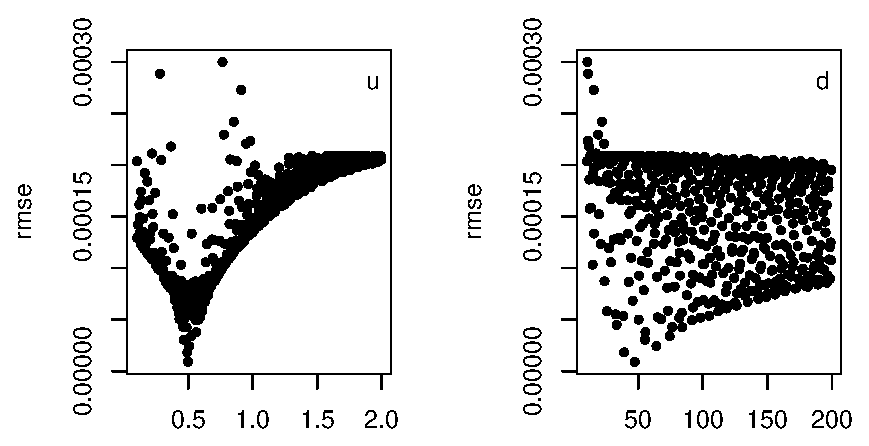
\includegraphics[width=0.9\columnwidth]{\figdir/mcs_example/dottyplots_originalRange.eps}
  \caption{Output graphics created by the R code from \figref{fig:mops:example_mcs:driver}. \label{fig:mops:example_mcs:dottyplots_originalRange}}
\end{figure}

\subsubsection*{Inspecting the output}

The graphical output from the R code (\figref{fig:mops:example_mcs:driver}) is presented in \figref{fig:mops:example_mcs:dottyplots_originalRange}. In this example with only two parameters ($u$ and $d$), some structure is visible in the plots of the marginal distributions. From the left sub-figure, one may conclude that a parameter value of $u \approx 0.5$ fits best with the observation data. The right sub-figure of \figref{fig:mops:example_mcs:dottyplots_originalRange} suggest that reasonable values for the dispersion coefficient $d$ are probably found in a range between 10 and 70. In order to refine the estimate, one could try different options:
\begin{enumerate}
  \item Re-run the Monte-Carlo experiment with narrower sampling ranges. For example, the sampling range for parameter $d$ could be restricted to 0 $\ldots$ 100. This option was already discussed in \secref{sec:mops:background:semiAutoCalib}. The result of such a re-run with narrowed sampling ranges is presented in \figref{fig:mops:example_mcs:dottyplots_narrowedRange}.
  \item Re-run the Monte-Carlo experiment with a higher number of random samples. 
  \item Use the current estimates of $u=0.5$ and $d=50$ as initial values for one of the true optimization algorithms provided by R's \texttt{optim} method.
\end{enumerate}

\begin{figure}
  \centering
  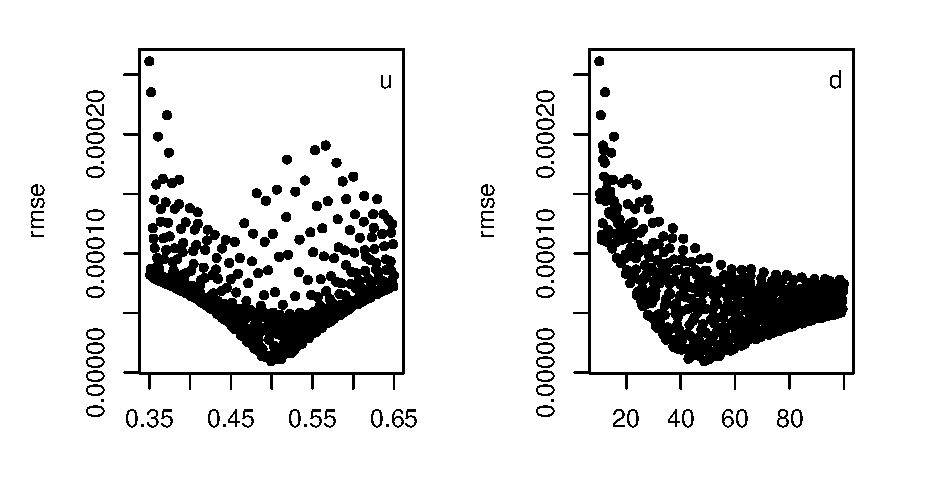
\includegraphics[width=0.9\columnwidth]{\figdir/mcs_example/dottyplots_narrowedRange.eps}
  \caption{Output graphics created by the R code from \figref{fig:mops:example_mcs:driver} after narrowing of the sampling ranges ($u$ in 0.35 $\ldots$ 0.65; $d$ in 10 $ \ldots$ 100). \label{fig:mops:example_mcs:dottyplots_narrowedRange}}
\end{figure}

%%%%%%%%%%%%%%%%%%%%%%%%%%%%%%%%%%%%%%%%%%%%%%%%%%%%%%%%%%%%%%%%%%%%%%%%%%%%%%%%
\section{Using \software{mops} with an \software{echse}-based model} \label{sec:mops:echse}

This section contains some practical hints for the use of \software{mops} together with an \software{echse}-based model. The hints refer in particular to the methods \texttt{modelError\_multiDim} and \texttt{modelError\_oneDim} which have many arguments in common.

\paragraph{Command line arguments} An \software{echse}-based model generally expects some mandatory command line arguments of the form 'key=value' \citep[see][for details]{Echse-Main-Doc}. All optional command line arguments (configuration data) are of the 'key=value' form as well. Therefore, the value assigned to the method's argument \texttt{model\_args} must always be a \emph{named} vector. A minimum exaple, covering only the mandatory command line arguments is given in \figref{fig:mops:echse:cmdArgs}.

\begin{figure}
\begin{lstlisting}[style=R]
model_args= c(file_control="myModel.cnf",
  file_log="myModel.log",
  file_err="errors.html",
  format_err="html", silent="true")
\end{lstlisting}
\caption{Example, demonstrating the use of the \texttt{model\_args} argument. \label{fig:mops:echse:cmdArgs}}
\end{figure}

\paragraph{Clean-up functions} An \software{echse}-based model never overwrites existing files. Therefore, when carrying out a series of model runs, there must be a mechanism to delete the output created by the previous run. By assigning a proper function to the arguments \texttt{func\_first} and an appropriate value to \texttt{moreArgs\_first} such an automatic clean-up may be accomplished. Alternatively, the clean-up may be done right after a model run, by supplying an appropriate function for \texttt{func\_final} and value for \texttt{moreArgs\_final}.

In some cases, a complete removal of the model outputs after each run may be undesired. For example, one might be interested in the actual time series output produced by the individual runs of a Monte-Carlo simulation. Then, renaming is usually an appropriate alternative to deletion of files. This can be done, for example, by supplying appropriate code as \texttt{func\_final} and a suitable value for \texttt{moreArgs\_final}. In those cases, it is often convenient to use a string representation of the system's time for the generation of unique file names.

\paragraph{Files created by the model} Output files created by an \software{echse}-based model conform to some simple standards which facilitates the use of \software{mops}. In all time series output files, the column with time information is named 'end\_of\_interval'. Thus, this is the string to be assigned to the argument \texttt{sim\_colTime} (\figref{fig:mops:echse:time}). Furthermore, the time information printed by \software{echse}-based models is always in ISO 8601 format (YYYY-MM-DD hh:mm:ss) with date and time separated by a single blank character. This is also the default format used by \software{mops}. Therefore, the actual argument for \texttt{sim\_timeConv} can be omitted in the call to methods like \texttt{modelError\_MCS}. If, even though, a time-conversion function is specified it should be defined as in \figref{fig:mops:echse:time}.

\begin{figure}
\begin{lstlisting}[style=R]
  sim_colTime=  "end_of_interval"
  sim_timeConv= function(x) {
    as.POSIXct(strptime(x,
    "%Y-%m-%d %H:%M:%S",tz="GMT"),
    tz="GMT")
    }
\end{lstlisting}
\caption{Appropriate values of the arguments \texttt{sim\_colTime} and \texttt{sim\_timeConv} when using \software{mops}'s methods with an \software{echse}-based model. \label{fig:mops:echse:time}}
\end{figure}

%%%%%%%%%%%%%%%%%%%%%%%%%%%%%%%%%%%%%%%%%%%%%%%%%%%%%%%%%%%%%%%%%%%%%%%%%%%%%%%%
\section{Troubleshooting} \label{sec:mops:troubleshooting}

\subsection{General recommendations} \label{sec:mops:troubleshooting:general}

The methods contained in the \software{mops} package perform quite complex tasks and there is a high potential for making mistakes. In many cases, the cause of failure should be obvious from the generated error messages. However, there are situations where it may be difficult to locate and identify the actual problem. Therefore, some general guidelines for troubleshooting are given in this section. More specific problems are addressed in \secref{sec:mops:troubleshooting:specific}.

If one of \software{mops}'s high-level methods involving a call to a simulation model fails, one should first try to find out at which step of the computation the problem occurred. There are four possible categories a--d with typical symptoms:

\subsubsection*{(a) Stop occurs prior to running the model}
\begin{itemize}
  \item The model does neither produce the desired output nor any other files (log files, files with error messages, etc.).
  \item A return code of the model is \emph{not} reported.
\end{itemize}

\subsubsection*{(b) Stop occurs when calling the model}
\begin{itemize}
 \item As in case (a), the model does not produce any output files.
  \item A \emph{non-zero} return code of the model \emph{is} reported.
\end{itemize}

\subsubsection*{(c) Stop occurs while running the model}
\begin{itemize}
  \item The model produces a file with error messages and/or a log file whose entries indicate early termination.
  \item A \emph{non-zero} return code of the model \emph{is} reported.
\end{itemize}

\subsubsection*{(d) Stop occurs after running the model}
\begin{itemize}
  \item The model produces the desired output files and possibly a complete log file.
  \item A return code of the model is \emph{not} reported.
\end{itemize}

Note that (b) is a quite common case. It typically occurs if the model is called with invalid or incomplete command line arguments. In case of \software{echse}-based models, it may happen that the model executable is called successfully but the names of the files for log info and diagnostic messages are not properly passed via the command line. Consequently, the model terminates without creating any log or error output. The non-zero return level is the only sign of failure then.

\subsection{Specific recommendations} \label{sec:mops:troubleshooting:specific}

\subsubsection*{The model does not run at all}
\begin{itemize}
  \item Check the path to the executable if a relative or absolute path was specified.
  \item If the executable is called just by its name but the file does not reside in R's working directory, you might need to check/adjust your 'PATH' environment variable.
  \item Check for broken links (if a link is used).
  \item Check whether the file is actually executable.
\end{itemize}

\subsubsection*{The command line is not passed to the model}
\begin{itemize}
  \item Try to call the executable directly, \ie{} not via an intermediate shell script and not using a link. This is best done by adding the directory containing the executable to the 'PATH' variable.
  \item If this does not help, replace the executable by a shell script that reports its full command line but does nothing else. Try to learn from this.
\end{itemize}

\subsubsection*{The model crashes due to floating point exceptions}

In true optimization as well as in Monte-Carlo simulation, the simulation model is run with many different parameter sets. In general, the tested parameter sets are chosen by the used algorithm, based on sophisticated rules or simply by random sampling. Thus, the particular sets are not know a-priori.

In many models, the values of different parameters are not totally independent. For example, if a fictive parameter 'maximumCapacity' has a value of 5, it does not make sense if a companion parameter 'minimumCapacity' has a value greater than 5. Similarly, some parameter values may be incompatible with the initial value(s) of state variable(s). If, for example, the fictive parameter 'minTemperature' has a value of 5, problems are waiting to happen if a related state variable 'temperature' is initialized to a value of 0.

The consequences are as follows:
\begin{itemize}
  \item When using one of \software{mops}'s methods together with a true optimization algorithm, it may be necessary to set box-constraints for critical parameters. Similarly, when doing Monte-Carlo simulations with the \texttt{modelError\_MCS} method, the sampling ranges must be chosen with care in order not to produce invalid (\eg{} unphysical) parameter combinations.
  \item The initial values for the state variables must be chosen so as to be compatible with any parameter sets possibly tested during optimization or Monte-Carlo simulation, respectively.
\end{itemize}

Disregard of this often causes a model to crash due to floating point exceptions. In other cases, the model only produces implausible outputs (which are hopefully detected because of a bad fit).




\chapter{Filling of gaps in meteorological time series (\software{meteofill})} \label{chap:meteofill}
\renewcommand{\tabdir}{chapters/meteofill/tab}
\renewcommand{\figdir}{chapters/meteofill/fig}

%%%%%%%%%%%%%%%%%%%%%%%%%%%%%%%%%%%%%%%%%%%%%%%%%%%%%%%%%%%%%%%%%%%%%%%%%%%%%%%%
%%%%%%%%%%%%%%%%%%%%%%%%%%%%%%%%%%%%%%%%%%%%%%%%%%%%%%%%%%%%%%%%%%%%%%%%%%%%%%%%
%%%%%%%%%%%%%%%%%%%%%%%%%%%%%%%%%%%%%%%%%%%%%%%%%%%%%%%%%%%%%%%%%%%%%%%%%%%%%%%%
\section{Purpose} \label{sec:meteofill:purpose}
For hydrological modeling, time series of meteorological variables are required. Besides rainfall, this usually includes variables like temperature, radiation, humidity, windspeed, and possibly air pressure. The time series of meteorological observations often containg some (or many) missing values due to failure of sensors, power blackout, errors in transmission and recording of data and various other causes.

Internally, all hydrological models require continuous (\ie{} gap-free) time series of the meteorological forcing variables. This requirement can be fulfilled in two different ways. In the first strategy (\figref{fig:meteofill:fill_alternatives}, left) the model reads the incomplete series and must fill the gaps internally. The second strategy (\figref{fig:meteofill:fill_alternatives}, right) uses an external pre-processor to complete the information before calling the model.

The second approach has a number of advantages listed below:

\begin{itemize}
  \item Models are often run many times using the same input data set (for example in calibration or uncertainty analysis). It would be a massive waste of computer time to repeatedly pre-process the time series input in every single run.
  \item Separating the time series pre-processor from the actual model makes the software more modular which is advantageous in terms of re-use and maintenance.
\end{itemize}

\begin{figure}
  \centering
  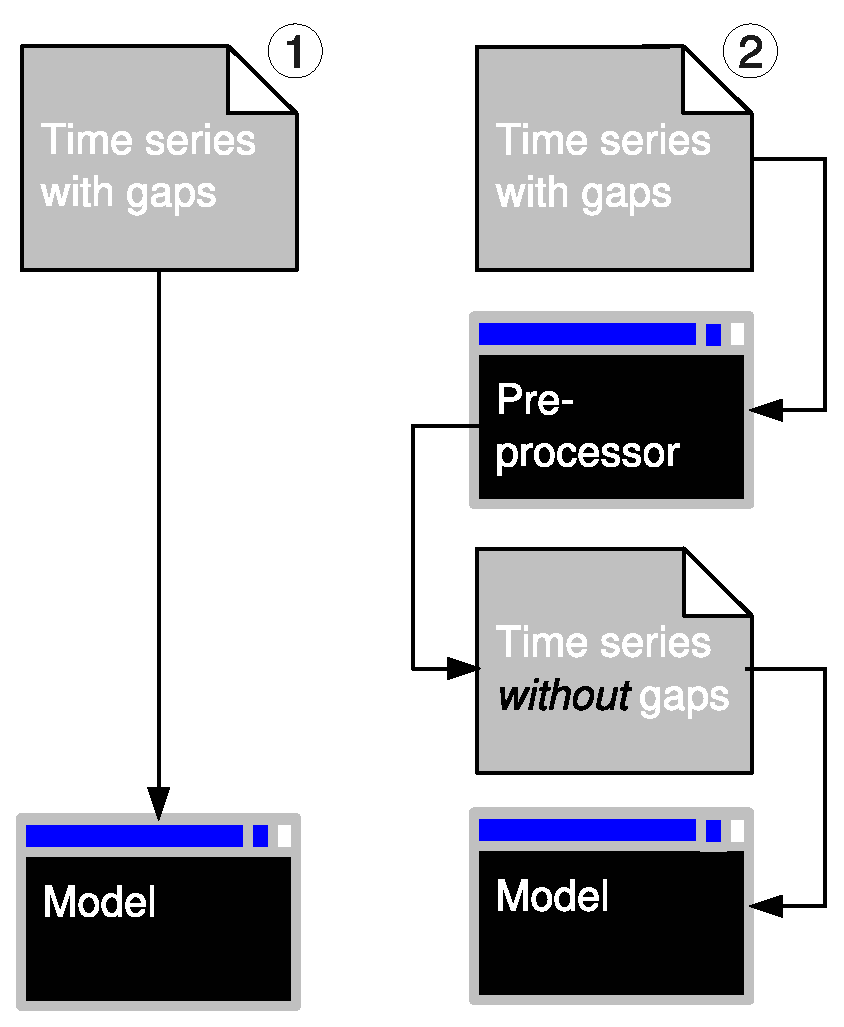
\includegraphics[width=0.65\columnwidth]{\figdir/fill_alternatives.eps}
  \caption{Alternative strategies to handle gaps a model's input time series. \label{fig:meteofill:fill_alternatives}}
\end{figure}

\software{meteofill} is designed for the second approach (\figref{fig:meteofill:fill_alternatives}, right). It is a pre-processor to produce gap-free time series from observation data.

The methodology used by \software{meteofill} is built on a space-for-time trade approach (see \secref{sec:meteofill:method}). It requires that observation data are available for \emph{multiple stations}. Using \software{meteofill} to fill gaps in a time series of observations at a single location is technically possible but it is likely to give poor result (see details in \secref{sec:meteofill:filling}).

Note that, for \emph{spatially distributed} models, there are now \emph{two separate steps of spatial interpolation}. In the first step, \software{meteofill} is uses spatial interpolation to remove any gaps in the model's multi-location input time series. In the second step, typically called regionalization, the pre-processed multi-location data are then interpolated to the spatially distributed model objects.

This second interpolation step is typically fully independent of \software{meteofill} and may be carried out, for example, by the simulation model, or any geostatistical software.

It is also possible, however, to use \software{meteofill} to combine the two steps of spatial interpolation mentioned above. This is illustrated in \figref{fig:meteofill:possibleUses}.

In the left branch of \figref{fig:meteofill:possibleUses}, \software{meteofill} is used to fill the gaps in time series of actual observations made at real-world stations. The distributed model reads the pre-processed time series and performs the regionalization to the model objects internally. In this approach, the model reads a rather small amount of data from files which is efficient with respect to computation time and disk space. User's of \software{echse}-based models propably always want to use this approach.

The alternative is shown in the right branch of \figref{fig:meteofill:possibleUses}, where \software{meteofill} is used as an all-in-one interpolation tool. This is practically achieved by considering the locations of the model objects as 'normal' observation sites \emph{that never recorded any data}. This kind of usage may be problematic for models with many spatially distributed objects, in particular if longer time series are processed. The produced files may become extremely large, which may result in a massive slow-down of model performance and disk operations in general. Thus, the use of \software{meteofill} as an all-in-one interpolation tool is recommended in special cases only (small models, few time steps; see example in \figref{fig:meteofill:resid}).

\begin{figure*}
  \centering
  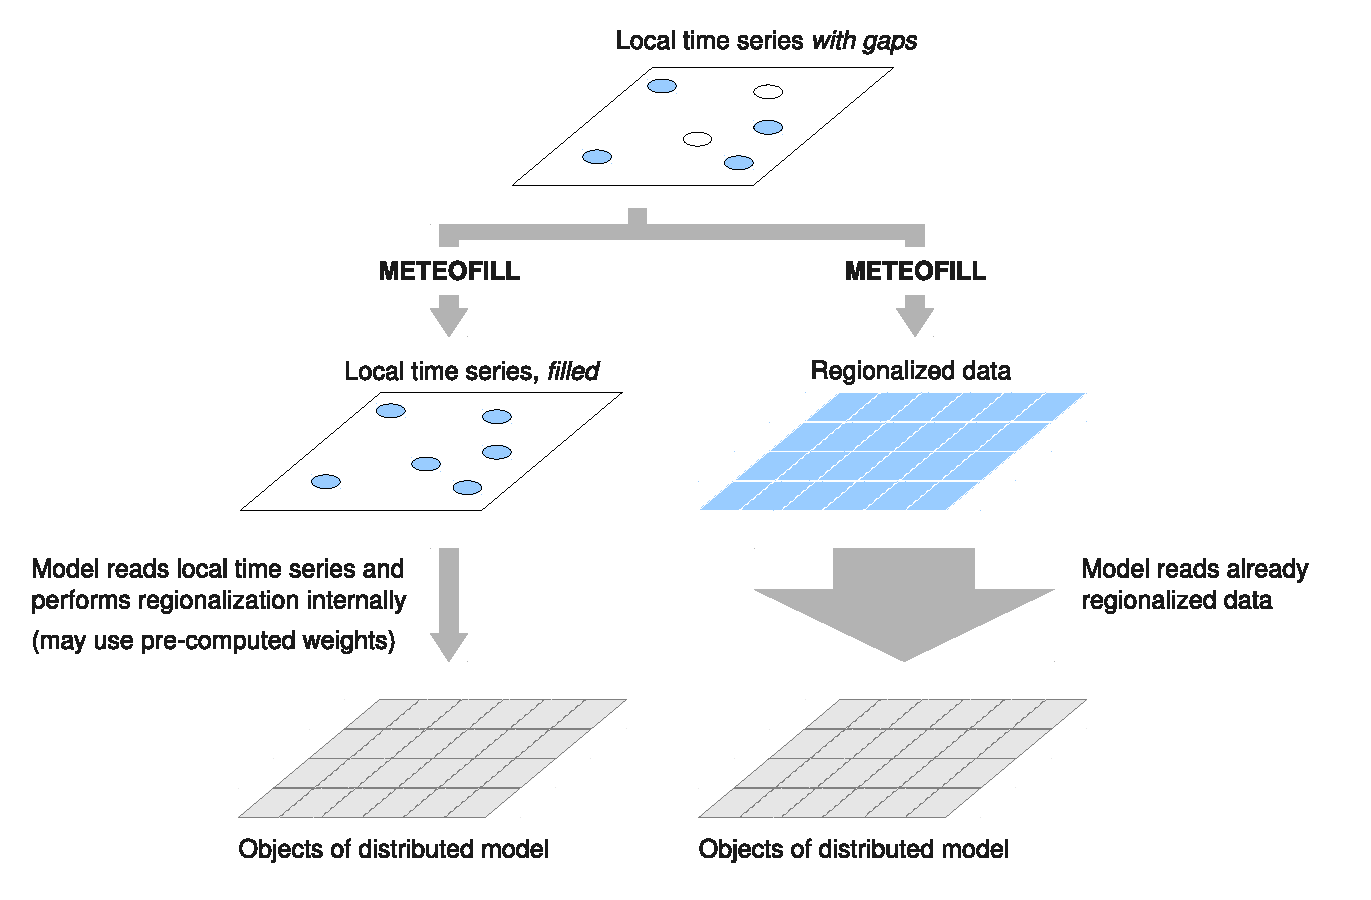
\includegraphics[width=0.8\textwidth]{\figdir/possibleUses.eps}
  \caption[Possible strategies of preparing the time series input of a spatially distributed model using \software{meteofill}]{Possible strategies of preparing the time series input of a spatially distributed model using \software{meteofill}. Whenever possible, the left branch should be preffered for performance reasons. \label{fig:meteofill:possibleUses}}
\end{figure*}

%%%%%%%%%%%%%%%%%%%%%%%%%%%%%%%%%%%%%%%%%%%%%%%%%%%%%%%%%%%%%%%%%%%%%%%%%%%%%%%%
%%%%%%%%%%%%%%%%%%%%%%%%%%%%%%%%%%%%%%%%%%%%%%%%%%%%%%%%%%%%%%%%%%%%%%%%%%%%%%%%
%%%%%%%%%%%%%%%%%%%%%%%%%%%%%%%%%%%%%%%%%%%%%%%%%%%%%%%%%%%%%%%%%%%%%%%%%%%%%%%%
\section{Methods} \label{sec:meteofill:method}

\subsection{Filling of gaps} \label{sec:meteofill:filling}
The approach taken by \software{meteofill} is best explained with an example (\figref{fig:meteofill:basics}). In order to substitute a missing data value (cross) by a reasonable estimate, one could, in theory:
\begin{enumerate}
  \item interpolate in time. For example, the missing value at location 3 in time step 4 could be substituted by interpolating between the values at the same location in time steps 3 and 5.
  \item assume persistence. For example, the missing value at location 3 in time step 4 could simply be substituted by the value from the previous time step (step 3, same location). This is actually a special case of interpolation in time, where the previous and next value are weighted with factors of 1 and 0, respectively.
  \item interpolate in space. For example, the missing values at locations 2 and 4 in time step 2 could be estimated by spatially interpolating the values from the remaining locations 1, 2, and 5 observed at the same time step.
  \item combine the ideas of spatial and temporal interpolation.
\end{enumerate}

\begin{figure}
  \centering
  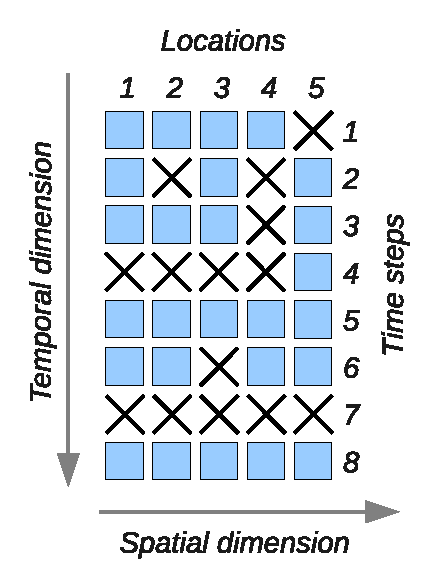
\includegraphics[width=0.55\columnwidth]{\figdir/basics.eps}
  \caption{Example of a multi-location times series of a meteorological variable with valid (squares) and missing data values (crosses). \label{fig:meteofill:basics}}
\end{figure}

The current version of \software{meteofill} primarily relies on \emph{spatial} interpolation, rather than interpolation in time. This can be summarizes by the following simple rules:
\begin{itemize}
  \item If, in a time step, a value is available at $n \geq 1$ location(s), missing data at the other $m$ locations are estimated by spatial interpolation (see \secsref{sec:meteofill:idw} and \ref{sec:meteofill:resid} for details). In the simplest case with $n=1$, the single observation is assumed to be valid globally.
  \item If, in a time step, no data are available at any location, persistence is assumed. Thus, for each location, the value (or estimate\footnote{If data are missing for a number of subsequent time steps}) from the previous time step is used (see \secref{sec:meteofill:hints:persistenceOptions} for practical advices).
\end{itemize}

After filling the gaps at all station in a time step $j$, the computation proceeds with time step $j+1$. This algorithm obviously requires that, in the very first time step, there is at least one location with a non-missing value.

\subsection{Inverse-distance approach} \label{sec:meteofill:idw}
The inverse-distance method (\eqnref{eqn:meteofill:idw}) is used to perform the spatial interpolation. It is a robust and computationally cheap method. To a limited extent, the spatial autocorrelation of the interpolated variable can be taken into account by adjustment of the exponent $p$ in \eqnref{eqn:meteofill:idw}.

\begin{equation}
y_k = \frac{\sum_{i=1}^{n} \left( y_i \cdot d(i,k)^{-p}\right)}{\sum_{i=1}^{n} \left( d(i,k)^{-p} \right)} \label{eqn:meteofill:idw}
\end{equation}

with

\begin{tabular}{lp{0.7\columnwidth}}
  $y_k$ & Value at the target location (index $k$). \\
  $y_i$ & Value at source location with index $i$. \\
  $d(i,k)$ & Distance between locations with indices $i$ and $k$. \\
  $p$ & Parameter (typically set to 2). \\
\end{tabular}

\medskip
For a particular target location (index $k$ in \eqnref{eqn:meteofill:idw}), the set of appropriate source locations (indices $1$ through $n$ in \eqnref{eqn:meteofill:idw}) is found by a sector search. Thus, the surrounding area of the location $k$ is dub-divided into a number of sectors and only the nearest source location is picked from each sector. This is illustrated in \figref{fig:meteofill:nearest}.

\begin{figure}
  \centering
  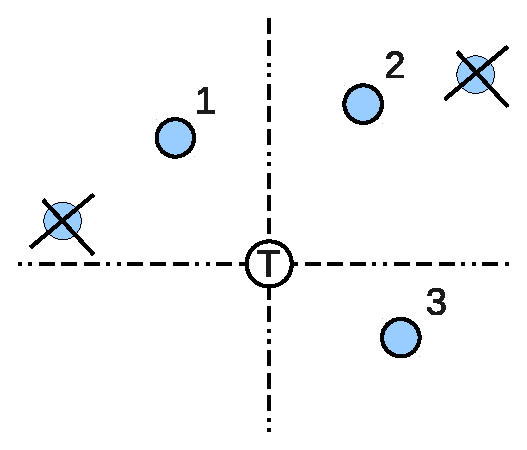
\includegraphics[width=0.55\columnwidth]{\figdir/interpolation_nearest.eps}
  \caption[Example of a sector search in spatial interpolation.]{Example of a sector search in spatial interpolation. From each of the four sectors, only the nearest station (1,2,3) is used in estimating the variable at the target location ($T$). Values at the crossed locations are neglected. \label{fig:meteofill:nearest}}
\end{figure}

Given a fixed number of sectors, the selection of the source location obviously depends on the orientation of the sectors. To achieve an optimum result, \software{meteofill} allows for testing different orientations by rotating the sectors (\figref{fig:meteofill:rotation}). From the tested orientations, \software{meteofill} uses the one where the cumulated distance between the target and the source locations is minimal.

\begin{figure}
  \centering
  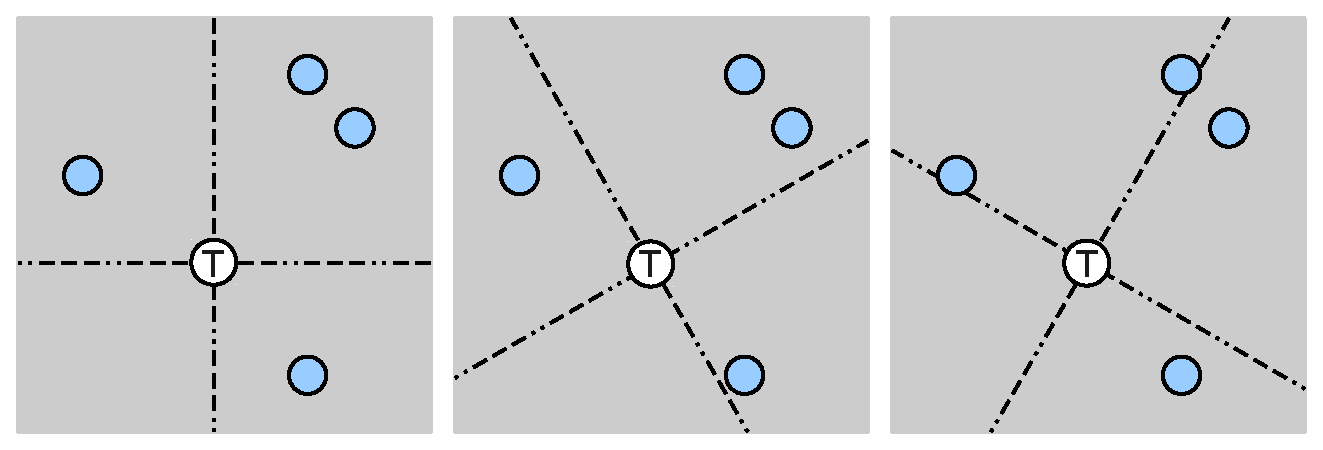
\includegraphics[width=0.95\columnwidth]{\figdir/interpolation_sectorrotation.eps}
  \caption[Example of sector rotation.]{Example of sector rotation. This example used a number of four sectors with 3 different orientations.  \label{fig:meteofill:rotation}}
\end{figure}

The selection of the appropriate source locations is the computationally most demanding step. This is especially so if both the number of target and source locations is large. Therefore, \software{meteofill} carries out a search for the source locations only
\begin{itemize}
  \item at the very beginning of the computation (first time step).
  \item if the set of locations with missing data has changed from the previous to the current time step.
\end{itemize}

\subsection{Residual interpolation} \label{sec:meteofill:resid}

The result of spatial interpolation can often be improved by using additional predictor variable(s). Values of these valiable(s) must be known at all source and target locations. For example, elevation my be a useful additional predictor when interpolating air pressure or temperature data. Two prominent approaches to spatial interpolation with additional predictors are (1) external drift Kriging and (2) residual interpolation.

\software{meteofill} supports the latter approach with the following settings/restrictions:
\begin{itemize}
  \item Only a \emph{single} predictor variable is supported.
  \item A \emph{linear} relation between the predictor and the interpolated variable is assumed.
  \item The \emph{additive} approach is used (not the alternative, multiplicative approach).
\end{itemize}

The basic algorithm of additive, uni-variate inverse-distance residual interpolation is summarized in \eqnsref{eqn:meteofill:resid_1} to \ref{eqn:meteofill:resid_3}

\begin{align}
y_k =& E_k + \frac{\sum_{i=1}^{n} \left( R_i \cdot d(i,k)^{-p}\right)}{\sum_{i=1}^{n} \left( d(i,k)^{-p} \right)} \label{eqn:meteofill:resid_1} \\
E_j =& a \cdot z_j + b \label{eqn:meteofill:resid_2} \\
R_i =& y_i - E_i \label{eqn:meteofill:resid_3}
\end{align}

with the additional symbols (cf. \eqnref{eqn:meteofill:idw})

\begin{tabular}{lp{0.7\columnwidth}}
  $E_j$ & Estimate of variable $y$ at an arbitrary location $j$ obtained from a linear model with the external predictor variable $z$ and empirical coefficients $a$ and $b$.  \\
  $R_i$ & Residual at a source location with index $i$. \\
\end{tabular}

The coefficients of the linear model (\eqnref{eqn:meteofill:resid_2}) are updated in every single time step. This is done using the data from all source locations (\ie{} all locations with valid data).

The linear correlation between the interpolated variable $y$ and the additional predictor variable $z$ may be more or less strong. In particular, the sign and quality of the correlation may be variable in time. Therefore, \software{meteofill} accepts a user-specified quality threshold, representing a minimum $R^2$. If the value of $R^2$ for the linear model (\eqnref{eqn:meteofill:resid_2}) is equal or greater than the user-specified threshold, residual interpolation is used (\eqnsref{eqn:meteofill:resid_1} to \ref{eqn:meteofill:resid_3}). Otherwise, in the case of a weak correlation, the plain inverse-distance method is applied (\eqnref{eqn:meteofill:idw}). The same is true if the number of data pairs for estimation of the linear model is lower than a user specified minimum sample size.

Residual interpolation is \emph{never} used if the threshold for $R^2$ is set to a value > 1 or if the minimum sample size is set to a value greater than the total number of locations.

In some cases, use of the linear model may result in undesired extrapolation effects. This is especially so, if
\begin{itemize}
  \item the range of possible values of the interpolated variable is limited. Example: Precipitation intensity cannot be negative.
  \item the value of the predictor variable $z$ at a target location is outside the range of $z$ values at the source locations. Example: Data are missing for a location at sea level and all available data correspond to elevations of 500--5000 meters.
\end{itemize}

In order to suppress such undesired results, \software{meteofill} allows for data truncation. The result values of residual interpolation are truncated if they are outside a user-specified range.

An example, illustrating the effect of residual interpolation in comparison with plain inverse-distance interpolation is shown in \figref{fig:meteofill:resid}.

\begin{figure*}
  \centering
  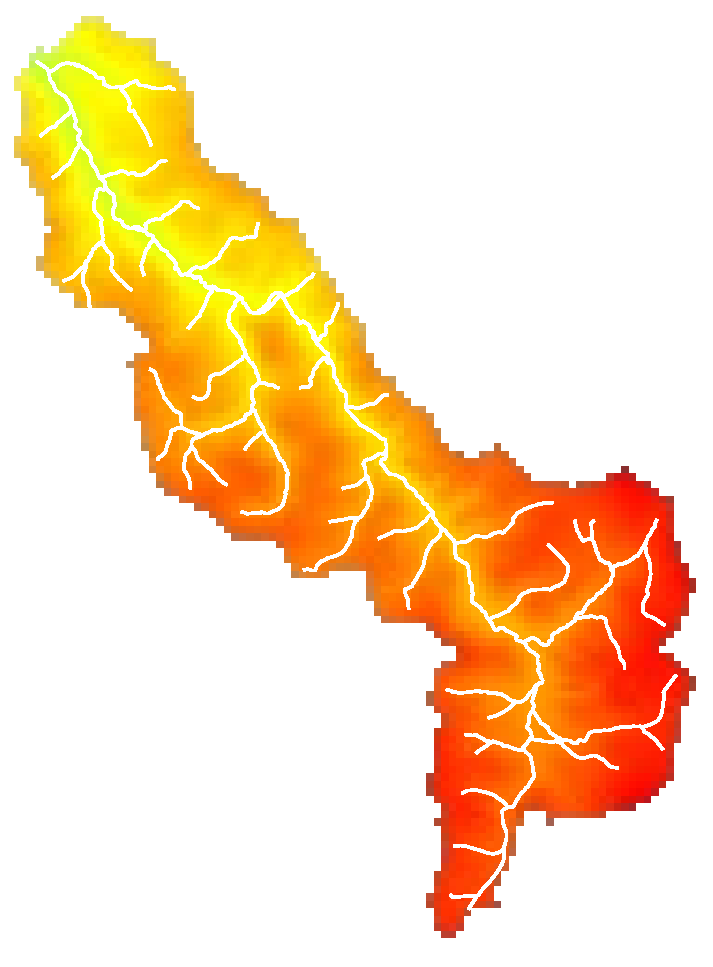
\includegraphics[width=0.3\textwidth, viewport=0 0 326 448, clip]{\figdir/demo/dem.eps}
  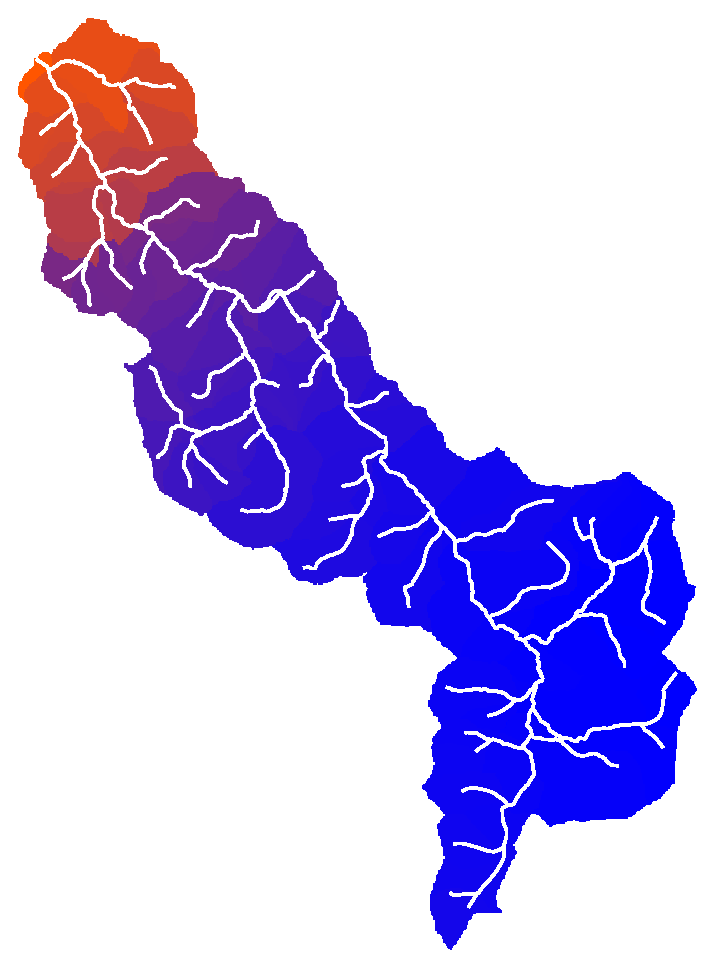
\includegraphics[width=0.3\textwidth, viewport=0 0 326 448, clip]{\figdir/demo/residInt_OFF.eps}
  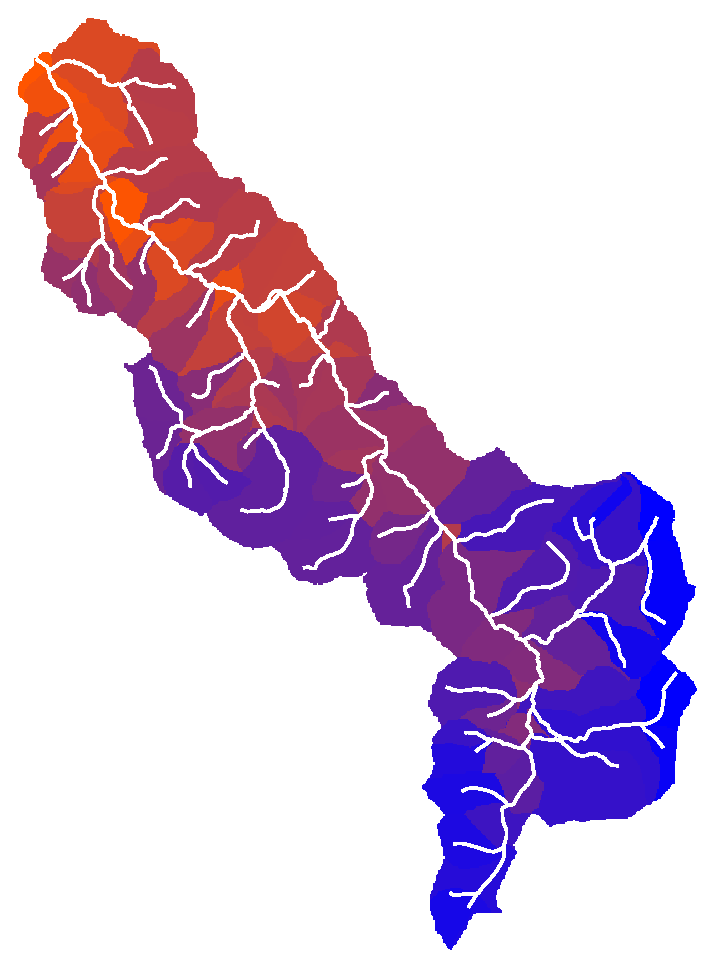
\includegraphics[width=0.3\textwidth, viewport=0 0 326 448, clip]{\figdir/demo/residInt_ON.eps}
  \caption[Example to illustrate the effect of residual interpolation.]{Effect of residual interpolation on the regionalization of air temperature in a mountainous watershed. In this example, the air temperature observed at climate stations is highly correlated to elevation. The stations (not shown) are located outside the watershed in the North (low elevation, warm) and South-East (high elevation, cold). Left: Elevation model (red: high, green: low) and river net (white). Center: \software{meteofill} output using the plain inverse-distance approach (blue: cold, red: warm). Right: \software{meteofill} output using residual interpolation with elevation as additional predictor. Obviously, higher temperatures are predicted in the valleys by taking the vertical temperature gradient into account. \label{fig:meteofill:resid}}
\end{figure*}

%%%%%%%%%%%%%%%%%%%%%%%%%%%%%%%%%%%%%%%%%%%%%%%%%%%%%%%%%%%%%%%%%%%%%%%%%%%%%%%%
%%%%%%%%%%%%%%%%%%%%%%%%%%%%%%%%%%%%%%%%%%%%%%%%%%%%%%%%%%%%%%%%%%%%%%%%%%%%%%%%
%%%%%%%%%%%%%%%%%%%%%%%%%%%%%%%%%%%%%%%%%%%%%%%%%%%%%%%%%%%%%%%%%%%%%%%%%%%%%%%%
\section{Arguments and invocation of \software{meteofill}} \label{sec:meteofill:args}

\software{meteofill} is an application written in C++. It expects all input to be supplied as command line arguments. All arguments must be supplied in a keyword-values style as in the following example call:

\begin{lstlisting}[style=shell]
meteofill ifile_locations="locations.txt"
  ifile_data="data_withGaps.txt"
  chars_colsep=" " chars_comment="#"
  nodata=-99. idw_power=2
  nsectors=4 norigins=3
  resid_nmin=3 resid_r2min=0.36
  resid_llim=-40. resid_ulim=40.
  ofile_data="data_filled.txt"
  ofile_locations="locations.txt"
  ndigits_max=1 logfile="log.txt"
  overwrite=true
\end{lstlisting}

The meaning of the various keywords is as follows:

\begin{columndef}
  \item[ifile\_locations] (\textit{string}) Input file listing the spatial coordinates for all locations. See \secref{sec:meteofill:input:locationsTable} for details.
  \item[ifile\_data] (\textit{string}) Input file with multi-location time series data. See \secref{sec:meteofill:input:timeSeries} for details.
  \item[chars\_colsep] (\textit{character(s)}) One or more character(s) used as a column-separator. Should be quoted, if a special character like TAB (ASCII code 9) is used. Any of the characters (if more than one) is treated as a column separator when reading input files. The columns of output files are separated by the first (or only) character in the set. Typically, a TAB character (enclosed by quotes) is used as in the above example.
  \item[chars\_comment] (\textit{character}) Initial character of comment lines in input files (typically the hash character). Should be quoted.
  \item[nodata] (\textit{numeric}) Value to indicate a missing value in the input time series. Typically, large negative values like -99 or -9999 are used for the common meteorological variables.
  \item[idw\_power] (\textit{numeric}) Value of parameter $p$ in \eqnref{eqn:meteofill:idw}. Typically a value of 1 or 2. The optimum value may be determined by cross-validation or variogram analysis.
  \item[nsectors] (\textit{integer}) Number of sectors to be used in the search of source locations (see \figref{fig:meteofill:nearest}). Using \texttt{nsectors=1} forces a nearest-neighbor interpolation. You probably want to use a value between 3 and 8 (or 1).
  \item[norigins] (\textit{integer}) The number of sector origins (sector rotations) to be tested. See \secref{sec:meteofill:idw} (\figref{fig:meteofill:rotation}). You probably want to use a value between 1 and 5. Larger values should give better results at the expense of an increase in computation time.
  \item[resid\_nmin] (\textit{integer}) Minimum number of locations with valid data (source locations) for possibly activation of residual interpolation. If the actual number of source locations is less than \verb!resid_nmin!, residual interpolation is \emph{not} used. Otherwise, the decision depends on the quality of the linear correlation (see \verb!resid_r2min!). Reasonable values for \verb!resid_nmin! are probably $\ge$ 3.
  \item[resid\_r2min] (\textit{numeric}) Minimum $R^2$ of the linear model used in residual interpolation (see \secref{sec:meteofill:resid}). For actual activation of residual interpolation, the computed $R^2$ for the particular time step must be $ge$ \verb!resid_r2min! and, \emph{in addition}, the sample size must be large enough (see \verb!resid_nmin!). Reasonable values for \verb!resid_r2min! are probably $\ge$ 0.36 (correlation coefficient of 0.6).
  \item[resid\_llim] (\textit{numeric}) Lower truncation limit in case of residual interpolation (see \secref{sec:meteofill:resid}). For variables that cannot take negative values (like precipitation or short-wave radiation), \verb!resid_llim! should be set to zero.
  \item[resid\_ulim] (\textit{numeric}) Upper truncation limit in case of residual interpolation (see \secref{sec:meteofill:resid}).
  \item[ofile\_data] (\textit{string}) Name/path of the output file containing the time series with all gaps filled according to the method described in \secref{sec:meteofill:method}.
  \item[ofile\_locations] (\textit{string}) Name/path of the output file containing a list of the locations from \verb!ifile_locations! for which data are actually present in \verb!ifile_data!.
  \item[logfile] (\textit{string}) Name/path of an output log file.
  \item[ndigits\_max] (\textit{integer}) Number of digits to be used in the output file \verb!ofile_data!.
  \item[overwrite] (\textit{logical}) A value of either true of false. If true, any existing output files will silently be replaced.
\end{columndef}

After successful execution, the return code of \software{meteofill} is zero. If the program terminates due to an error, a non-zero code is returned and traceback info is sent to standard output.

%%%%%%%%%%%%%%%%%%%%%%%%%%%%%%%%%%%%%%%%%%%%%%%%%%%%%%%%%%%%%%%%%%%%%%%%%%%%%%%%
%%%%%%%%%%%%%%%%%%%%%%%%%%%%%%%%%%%%%%%%%%%%%%%%%%%%%%%%%%%%%%%%%%%%%%%%%%%%%%%%
%%%%%%%%%%%%%%%%%%%%%%%%%%%%%%%%%%%%%%%%%%%%%%%%%%%%%%%%%%%%%%%%%%%%%%%%%%%%%%%%
\section{Input} \label{sec:meteofill:input}

\subsection{Locations table} \label{sec:meteofill:input:locationsTable}
The locations table is a text file with four columns (see \secref{sec:meteofill:args} for how to select a column separator). The expected column names are \texttt{id}, \texttt{x}, \texttt{y}, and \texttt{z}. The \texttt{id} column contains the names of locations (usually climate stations or rain gages), for which data are available. The IDs are read as strings. The corresponding spatial coordinates go in the \texttt{x} and \texttt{y} fields. For the coordinates one should use a \emph{geodetic} system (\ie{} units of meters, kilometers, miles, etc.). The \texttt{z} field should contain the values of the external predictor variable for residual interpolation. Elevation is the natural choice if nothing better is available. If residual interpolation should not be used anyway, the \texttt{z} column may be filled with dummy values.

An example of a locations table is given in \figref{fig:meteofill:input:locationsTable}.

\begin{figure}
\begin{lstlisting}[style=txt]
id	x	y	z
klotzsche	4623183	5667440	227
hosterwitz	4629789	5655359	114
strehlen	4623996	5652991	119
dipps_rein	4620226	5644000	365
zinnwald	4623539	5622933	877
\end{lstlisting}
  \caption{Example of a locations table. \label{fig:meteofill:input:locationsTable}}
\end{figure}

It is OK if the locations table contains more than the mandatory columns. \software{meteofill} simply ignores the unnecessary information. It is also OK if the locations table contains records for additional locations not present in the time series input file (\secref{sec:meteofill:input:timeSeries}). These records are silently ignored as well.

\subsection{Time series file} \label{sec:meteofill:input:timeSeries}
The time series input file is a text file with $n+1$ columns where $n$ is the number of locations (see \secref{sec:meteofill:args} for how to select a column separator). The table must have a header line with column names.
The first column of the file is expected to contain time information in ascending order (oldest record first). Any format can be used as \software{meteofill} internally treats the data as strings, not as times. For this first column, an arbitrary name can be chosen (but it must be present).
The remaining $n$ columns contain the numeric observation data at the $n$ locations. These columns may be in any order but their names need to match exactly with the location IDs provided in the locations table (\secref{sec:meteofill:input:locationsTable}). Any missing or invalid data values must be indicated by the \texttt{nodata} value (see \secref{sec:meteofill:args}). An example of multi-location time series file is given in \figref{fig:meteofill:input:timeSeries}.

\begin{figure}
\begin{lstlisting}[style=txt]
time	MT.CMP.	ARIES	MT.ORO
2000-01-01	0	-99	0
2000-01-02	4	-99	1
2000-01-03	12	3	1
2000-01-04	-99	-99	-99
2000-01-05	0	-99	0
\end{lstlisting}
  \caption{Example of multi-location time series file for use with \software{meteofill}. \label{fig:meteofill:input:timeSeries}}
\end{figure}

For the algorithm to be successful, it is important that the very first (oldest) record contains valid data for one location, at least.

%%%%%%%%%%%%%%%%%%%%%%%%%%%%%%%%%%%%%%%%%%%%%%%%%%%%%%%%%%%%%%%%%%%%%%%%%%%%%%%%
%%%%%%%%%%%%%%%%%%%%%%%%%%%%%%%%%%%%%%%%%%%%%%%%%%%%%%%%%%%%%%%%%%%%%%%%%%%%%%%%
%%%%%%%%%%%%%%%%%%%%%%%%%%%%%%%%%%%%%%%%%%%%%%%%%%%%%%%%%%%%%%%%%%%%%%%%%%%%%%%%
\section{Output} \label{sec:meteofill:output}
The current version of \software{meteofill} generates three output files whose names are specified at the command line (see \secref{sec:meteofill:args}). The contents of the files is described in \tabref{tab:meteofill:output}.

\begin{table*}
  \caption[Output files of \software{meteofill}.]{Output files of \software{meteofill}. The entries in the 'File' column refer to the command line arguments describe in \secref{sec:meteofill:args}. \label{tab:meteofill:output}}
  \begin{tabular}{p{0.2\textwidth} p{0.75\textwidth}} \hline\hline
    File & Contents \\ \hline
    \verb!ofile_data! & A multi-location time series table. Format and contents are identical to the input time series \secref{sec:meteofill:input:timeSeries} except that all \texttt{nodata} values are replaced by estimates according to \secref{sec:meteofill:method}. \\
    \verb!ofile_locations! & Similar to the input locations table described in \secref{sec:meteofill:input:locationsTable}. The table contains only the mandatory columns and list only those stations for which time series data are actually present. \\
    \verb!logfile! & Lists, for each time step, the number of locations with valid data (as absolute number in column \texttt{numdata} and as a percentage in column \texttt{availability}. The column \texttt{config\_changed} contains information on whether the set of locations with missing data has changed in comparison to the previous time step (requiring a new search for neighbored locations). The columns \texttt{residual\_interp} and \texttt{r2} contain information on the use of residual interpolation (true/false) and the corresponding $R^2$ of the linear model. \\ \hline\hline
  \end{tabular}
\end{table*}

%%%%%%%%%%%%%%%%%%%%%%%%%%%%%%%%%%%%%%%%%%%%%%%%%%%%%%%%%%%%%%%%%%%%%%%%%%%%%%%%
%%%%%%%%%%%%%%%%%%%%%%%%%%%%%%%%%%%%%%%%%%%%%%%%%%%%%%%%%%%%%%%%%%%%%%%%%%%%%%%%
%%%%%%%%%%%%%%%%%%%%%%%%%%%%%%%%%%%%%%%%%%%%%%%%%%%%%%%%%%%%%%%%%%%%%%%%%%%%%%%%
\section{Hints for practical usage} \label{sec:meteofill:hints}

\subsection{Missing-only data (options beyond persistence)} \label{sec:meteofill:hints:persistenceOptions}
As pointed out in \secref{sec:meteofill:filling}, \software{meteofill} assumes persistence if, in a particular time step, no data are available for any station (let's call this situation a \emph{global gap}). Although persistence is a simple and intuitive approach, it is likely to give satisfactory results only as long as the period of missing-only data is short enough. For long-lasting global gaps, persistence may not be a suitable assumption and it may be desireable to fill the gap with predefined values. Possible candidates are monthly average values or, in the case of rainfall data, a fixed value of zero.

Furtunately, there is a simple trick to let \software{meteofill} fill such global gaps with predefined values. All you need to do is to supplement the input data with a \emph{synthetic} station that 'recorded' the desired fill-in values (which may vary in time). The spatial coordinates of that synthetic station must be chosen so that it is \emph{very far} away from all the actual stations (\eg{} some million kilometers). Hereby it is ensured that the data from the synthetic station will practically be ignored (\ie{} weighted with almost zero), as long as any of the actual stations provides valid data.


\chapter{River cross-section analysis (\software{xsAnalyzer})} \label{chap:xsanalyzer}
\renewcommand{\tabdir}{chapters/xsAnalyzer/tab}
\renewcommand{\figdir}{chapters/xsAnalyzer/fig}

%%%%%%%%%%%%%%%%%%%%%%%%%%%%%%%%%%%%%%%%%%%%%%%%%%%%%%%%%%%%%%%%%%%%%%%%%%%%%%%%
%%%%%%%%%%%%%%%%%%%%%%%%%%%%%%%%%%%%%%%%%%%%%%%%%%%%%%%%%%%%%%%%%%%%%%%%%%%%%%%%
%%%%%%%%%%%%%%%%%%%%%%%%%%%%%%%%%%%%%%%%%%%%%%%%%%%%%%%%%%%%%%%%%%%%%%%%%%%%%%%%
\section{Purpose} \label{sec:xsanalyzer:purpose}
The \software{xsAnalyzer} software computes basic hydraulic properties of a river reach being described by
\begin{enumerate}
  \item a representative cross-section geometry,
  \item the hydraulic roughness (energy loss parameter),
  \item the bed slope,
  \item the reach length.
\end{enumerate}

The computed results refer to a situation of steady uniform flow. This means that (1) the flow rate is constant in time, (2) the cross-section geometry does not change along the reach, and (3) the slope of the water surface is identical to the bed slope (no backwater).

The \software{xsAnalyzer} tool can be used, for example, to
\begin{itemize}
  \item calculate an approximate rating curves for ungaged sites at a river,
  \item estimate parameters to describe a reach's retention characteristics for use by hydrologic flood routing methods.
\end{itemize}

Note that the R-package \software{topocatch} (see \chapref{chap:topocatch}) contains methods to perform similar tasks. However, as opposed to \software{xsAnalyzer} these methods are not capable of handling compound cross-sections, \ie{} those with a variable roughness (see \secref{sec:xsanalyzer:method}).

%%%%%%%%%%%%%%%%%%%%%%%%%%%%%%%%%%%%%%%%%%%%%%%%%%%%%%%%%%%%%%%%%%%%%%%%%%%%%%%%
%%%%%%%%%%%%%%%%%%%%%%%%%%%%%%%%%%%%%%%%%%%%%%%%%%%%%%%%%%%%%%%%%%%%%%%%%%%%%%%%
%%%%%%%%%%%%%%%%%%%%%%%%%%%%%%%%%%%%%%%%%%%%%%%%%%%%%%%%%%%%%%%%%%%%%%%%%%%%%%%%
\section{Methods} \label{sec:xsanalyzer:method}

The most important input information of \software{xsAnalyzer} is the cross-section geometry. \figref{fig:xsanalyzer:geometry} shows a typical example with a distinction between the main channel and the flood plains on either side of the river.

\begin{figure}
  \centering
  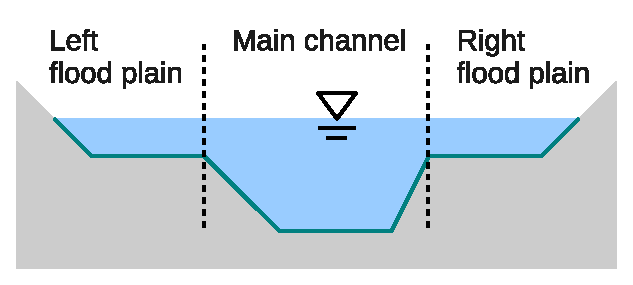
\includegraphics[width=0.55\columnwidth]{\figdir/xs-geometry-simple.eps}
  \caption{A typical river cross-section. \label{fig:xsanalyzer:geometry}}
\end{figure}

The cross-sections's geometry can be represented as a two column table. One column specifies the offset from a fixed point (typically at the left bank) and the other column holds the corresponding elevations. From such a table, the functions $A(D)$ and $R(D)$ can instantly be computed, where $D$ is the maximum flow depth in the cross-section, $A$ is cross-sections the wet area, and $R$ is the hydraulic radius (wet area divided by the wet perimeter).

Using Manning's equation (\eqnref{eqn:xsanalyzer:manning}), the flow rate for steady uniform conditions $Q$ can be calculated for a given flow depth $D$ if the slope $S$ and the roughness parameter $n$ are known. The reverse computation aimed at finding the value of $D$ for a given $Q$ is also possible but requires a numerical solution.

\begin{equation}
  Q(D) = \frac{1}{n} \cdot \sqrt{S} \cdot A(D) \cdot R(D)^{2/3} \label{eqn:xsanalyzer:manning}
\end{equation}

For many real-world cross-sections, the use of a single, unique roughness parameter $n$ is not appropriate. This is often the case for cross-sections with flood plains (\figref{fig:xsanalyzer:geometry}) because the actual surface roughness is horizontally variable. For example, the flood plains may be covered by vegetation while the bed of the main channel is made of sand or concrete. Then, energy losses due to turbulence will be quite different in the channel and the flood plains.

To handle this situation, \software{xsAnalyzer} uses the idea of compound cross-sections \citep[see][]{Cunge1980}. Thus, the cross-section is horizontally sub-divided into separate zones. To each zone, a unique value of $n$ is applied when using \eqnref{eqn:xsanalyzer:manning}. In the case shown in \figref{fig:xsanalyzer:geometry}, for example, the flow rate would be computed in two steps. First, the individual flow rates of the main channel and the two flood plains would be calculated, before the three values are added up in a second step.

It is important to keep in mind that this approach allows for different flow velocities in the zones. In reality, this would lead to additional turbulence and, consequently, result in additional energy losses due to shear at the zones' interface (\figref{fig:xsanalyzer:shear}). Such losses, however, are difficult to estimate and they are \emph{totally neglected} by \software{xsAnalyzer}.

\begin{figure}
  \centering
  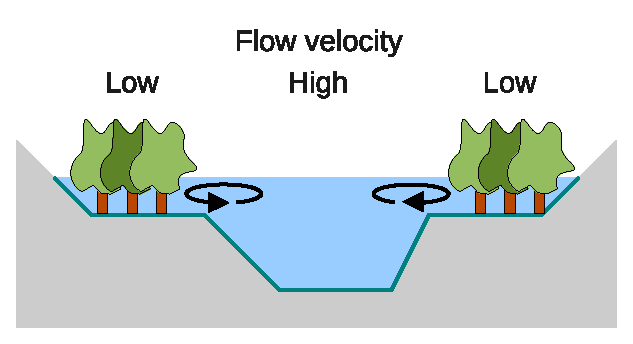
\includegraphics[width=0.55\columnwidth]{\figdir/xs-geometry-shear.eps}
  \caption{Turbulence due to shear at the interface of flow zones. \label{fig:xsanalyzer:shear}}
\end{figure}

If \software{xsAnalyzer} detects a water surface elevation which is higher than the cross-section's elevation at the first and/or last offset, it assumes a vertical wall at the respective offset. The output file (\secref{sec:xsanalyzer:output}) contains a field to detect those critical situations.

%%%%%%%%%%%%%%%%%%%%%%%%%%%%%%%%%%%%%%%%%%%%%%%%%%%%%%%%%%%%%%%%%%%%%%%%%%%%%%%%
%%%%%%%%%%%%%%%%%%%%%%%%%%%%%%%%%%%%%%%%%%%%%%%%%%%%%%%%%%%%%%%%%%%%%%%%%%%%%%%%
%%%%%%%%%%%%%%%%%%%%%%%%%%%%%%%%%%%%%%%%%%%%%%%%%%%%%%%%%%%%%%%%%%%%%%%%%%%%%%%%
\section{Arguments and invocation of \software{xsAnalyzer}} \label{sec:xsanalyzer:args}

\software{xsAnalyzer} is an application written in C++. It expects all input to be supplied as command line arguments. All arguments must be supplied in a keyword-values style as in the following example call:

\begin{lstlisting}[style=shell]
xsAnalyzer file_xsection="geometry.txt"
  file_flows="flowsOfInterest.txt"
  file_out="output.txt"
  read_3d=false
  read_roughness=false
  default_roughness=30
  slope=0.000485
  plain_length=1000.
  max_nreserv_kalmil=100
  print_only_routing=false
\end{lstlisting}

The meaning of the various keywords is as follows:

\begin{columndef}
  \item[file\_xsection] (\textit{string}) Input file with cross-section geometry data. See \secref{sec:xsanalyzer:input:geometry} for details.
  \item[file\_flows] (\textit{string}) Input file listing flow rates of interest. See \secref{sec:xsanalyzer:input:flows} for details.
  \item[file\_out] (\textit{string}) File name/path for output.
  \item[read\_3d] (\textit{logical}) Must be \false{} if the geometry data are given as a table of corresponding offsets and elevations. Must be \true{} if the geometry data are available as 3-dimensional coordinates.
  \item[read\_roughness] (\textit{logical}) Must be \true{} if the table with geometry data contains an additional column with roughness values. Note that the roughness must be specified as Strickler's $Kst$ parameter which is the inverse of Manning's $n$ ($Kst = 1/n$). If \false{}, a unique roughness value is assumed (see next argument).
  \item[default\_roughness] (\textit{numeric}) The unique value of the roughness parameter to be used if no values are specified in the geometry file. Note that the roughness must be specified as Strickler's $Kst$ parameter which is the inverse of Manning's $n$ ($Kst = 1/n$).
  \item[slope] (\textit{numeric}) Slope of the river bed as a dimensionless number (\ie{} meters elevation per meters distance).
  \item[plain\_length] (\textit{numeric}) Length of the reach as a horizontal distance. For typical values of the slope, this is almost identical to the actual length of the reach. 
  \item[max\_nreserv\_kalmil] (\textit{integer}) A parameter to control the output. It specifies the maximum number of conceptual linear reservoirs for the Kalinin-Miljukov routing method.
  \item[print\_only\_routing] (\textit{logical}) A switch to optionally reduce the amount of output information.
\end{columndef}

After successful execution, the return code of \software{xsAnalyzer} is zero. If the program terminates due to an error, a non-zero code is returned and traceback info is sent to standard output.

%%%%%%%%%%%%%%%%%%%%%%%%%%%%%%%%%%%%%%%%%%%%%%%%%%%%%%%%%%%%%%%%%%%%%%%%%%%%%%%%
%%%%%%%%%%%%%%%%%%%%%%%%%%%%%%%%%%%%%%%%%%%%%%%%%%%%%%%%%%%%%%%%%%%%%%%%%%%%%%%%
%%%%%%%%%%%%%%%%%%%%%%%%%%%%%%%%%%%%%%%%%%%%%%%%%%%%%%%%%%%%%%%%%%%%%%%%%%%%%%%%
\section{Input} \label{sec:xsanalyzer:input}

\subsection{Geometry data} \label{sec:xsanalyzer:input:geometry}
The file holding the geometry data must be in tabular format with columns separated by the TAB character (ASCII character code 9). Lines with an initial \verb!#! character are treated as comment lines. A header line with column names is mandatory. See the examples below for the expected column names.

\figsref{fig:xsanalyzer:input:geometry-2D-withoutRoughness} -- \ref{fig:xsanalyzer:input:geometry-3D-withRoughness} illustrate the four different possible file formats for geometry data. If the data are given in 2-dimensional format, the offsets must be in increasing order.

Note that, of roughness information is present, the value for a particuar offset applies to the part of the cross-section between this offset and the following offset. Thus, the roughness information of the very last record is effectively ignored (but a value must be present).

\begin{figure}
\begin{lstlisting}[style=txt]
  offset   z
  -100     20
  0        20
  5        15
  25       15
  30       20
  100      20
\end{lstlisting}
  \caption{Example of geometry file in 2D format without roughness information. \label{fig:xsanalyzer:input:geometry-2D-withoutRoughness}}
\end{figure}

\begin{figure}
\begin{lstlisting}[style=txt]
  offset   z     Kst
  -100     20    20
  0        20    30
  5        15    30
  25       15    30
  30       20    20
  100      20    20
\end{lstlisting}
  \caption{Example of geometry file in 2D format with specified roughness. \label{fig:xsanalyzer:input:geometry-2D-withRoughness}}
\end{figure}

\begin{figure}
\begin{lstlisting}[style=txt]
  x      y   z
  -100   0   20
  0      0   20
  5      0   15
  25     0   15
  30     0   20
  100    0   20
\end{lstlisting}
  \caption{Example of geometry file in 3D format without roughness information. \label{fig:xsanalyzer:input:geometry-3D-withoutRoughness}}
\end{figure}

\begin{figure}
\begin{lstlisting}[style=txt]
  x      y   z     Kst
  -100   0   20    20
  0      0   20    30
  5      0   15    30
  25     0   15    30
  30     0   20    20
  100    0   20    20
\end{lstlisting}
  \caption{Example of geometry file in 3D format with specified roughness. \label{fig:xsanalyzer:input:geometry-3D-withRoughness}}
\end{figure}

\subsection{Flow values of interest} \label{sec:xsanalyzer:input:flows}
The flow data are read from a plain text file like the one in \figref{fig:xsanalyzer:input:flows}. This is effectively a single-column table. A header must not be present. The user is free to specify a list of flow values with arbitrary increments but the data must be in increasing order.

\begin{figure}
\begin{lstlisting}[style=txt]
0.1
1
2
5
10
50
100
\end{lstlisting}
  \caption{Example of file with flow data for use with \software{xsAnalyzer}. \label{fig:xsanalyzer:input:flows}}
\end{figure}

\subsection{Units} \label{sec:xsanalyzer:input:units}
Note that the units of all input data need to be consistent. If, for example, the offsets are given in meters, the elevation data must be provided in units of meters too. At the same time, flow rates must be given in units of \cbm{} per second.

%%%%%%%%%%%%%%%%%%%%%%%%%%%%%%%%%%%%%%%%%%%%%%%%%%%%%%%%%%%%%%%%%%%%%%%%%%%%%%%%
%%%%%%%%%%%%%%%%%%%%%%%%%%%%%%%%%%%%%%%%%%%%%%%%%%%%%%%%%%%%%%%%%%%%%%%%%%%%%%%%
%%%%%%%%%%%%%%%%%%%%%%%%%%%%%%%%%%%%%%%%%%%%%%%%%%%%%%%%%%%%%%%%%%%%%%%%%%%%%%%%
\section{Output} \label{sec:xsanalyzer:output}
The current version of \software{xsAnalyzer} generates a single output file containing a summary of the properties of the cross-section / reach. An example is shown in \figref{fig:xsanalyzer:output}.

\begin{sidewaysfigure*}
{\small
\begin{lstlisting}[style=txt]
# Cross-section property table          
#   X-section data file:    in/montalban/geometry_constRough.txt          
#   Flow data file:         in/montalban/flowsOfInterest.txt          
#   Used reach length:      1000          
#   Used slope:             0.000485          
#   Used roughness: 30 (Global default)          
flow stage overtop wet_area top_width wet_perimeter volume_total dvdq_total nsub volume_sub dvdq_sub
0.5  19.74 0       1.71     5.6       5.79          1707.2       2231.8     3    569.1      743.9
1    19.92 0       2.82     6.94      7.19          2823.1       2111.8     2    1411.6     1055.9
2    20.16 0       4.69     8.74      9.07          4694.9       1915.7     1    4694.9     1915.7
5    20.64 0       10.84    18.02     18.57         10836.9      1932.4     1    10836.9    1932.4
10   21.02 0       19.54    27.94     28.67         19541.2      1553.4     1    19541.2    1553.4
20   21.41 0       31.33    32.13     32.98         31326.8      1175.3     1    31326.8    1175.3
30   21.75 0       43.05    38.84     39.73         43046.2      1310.8     1    43046.2    1310.8
50   22.33 0       74.82    72.4      73.55         74819.0      1302.6     1    74819.0    1302.6
75   22.64 0       98.45    78.1      79.51         98446.4      849.8      1    98446.4    849.8
100  22.88 0       117.31   78.32     80.04         117309.9     727.7      1    117309.9   727.7
\end{lstlisting}
}
  \caption{Example of an output file produced by \software{xsAnalyzer}. \label{fig:xsanalyzer:output}}
\end{sidewaysfigure*}

The meaning of the columns is as follows:
\begin{columndef}
  \item[flow] Flow rates of interest as specified in the input file.
  \item[stage] Water surface elevations corresponding to the flow rates of interest.
  \item[overtop] Either 0 or 1. A value of 1 means that the water surface elevation is higher than the cross-sections elevation at the first and/or last offset. In that case, a vertical wall was assumed as a boundary.
  \item[wet\_area] Wet cross-section area.
  \item[top\_width] Cross-section top width.
  \item[wet\_perimeter] Wetted perimeter.
  \item[volume\_total] Total storage volume of the reach.
  \item[dvdq\_total] Estimated derivative of the storage volume with respect to the flow rate.
  \item[nsub] Suggested number of linear reservoirs (= length of cascade) for Kalinin-Miljukov routing.
  \item[volume\_sub] Storage volume in the individual reservoirs for Kalinin-Miljukov routing.
  \item[dvdq\_sub] Estimated derivative of the storage volume with respect to the flow rate for the individual reservoirs for Kalinin-Miljukov routing. 
\end{columndef}


\newcommand{\tsplot}{\textsc{Tsplot}}

\chapter{Time series visualization tool (\software{tsplot})} \label{chap:tsplot}
\renewcommand{\tabdir}{chapters/tsplot/tab}
\renewcommand{\figdir}{chapters/tsplot/fig}

%%%%%%%%%%%%%%%%%%%%%%%%%%%%%%%%%%%%%%%%%%%%%%%%%%%%%%%%%%%%%%%%%%%%%%%%%%%%%%%%
%%%%%%%%%%%%%%%%%%%%%%%%%%%%%%%%%%%%%%%%%%%%%%%%%%%%%%%%%%%%%%%%%%%%%%%%%%%%%%%%
%%%%%%%%%%%%%%%%%%%%%%%%%%%%%%%%%%%%%%%%%%%%%%%%%%%%%%%%%%%%%%%%%%%%%%%%%%%%%%%%
\section{Purpose} \label{sec:tsplot:purpose}
\software{tsplot} is a lightweight tool for the interactive visualization of time series data. It offers a convenient way to quickly inspect the output of an \software{echse}-based simulation model. It is particularly useful for showing simulated and observed data in a single plot for the purpose of comparison (see \figref{fig:tsplot:example}).
Note that \software{tsplot} is optimized for interactive plotting only. If you need to create plots for presentation in a paper, for example, you better use R commands or another software.

\begin{figure*}
  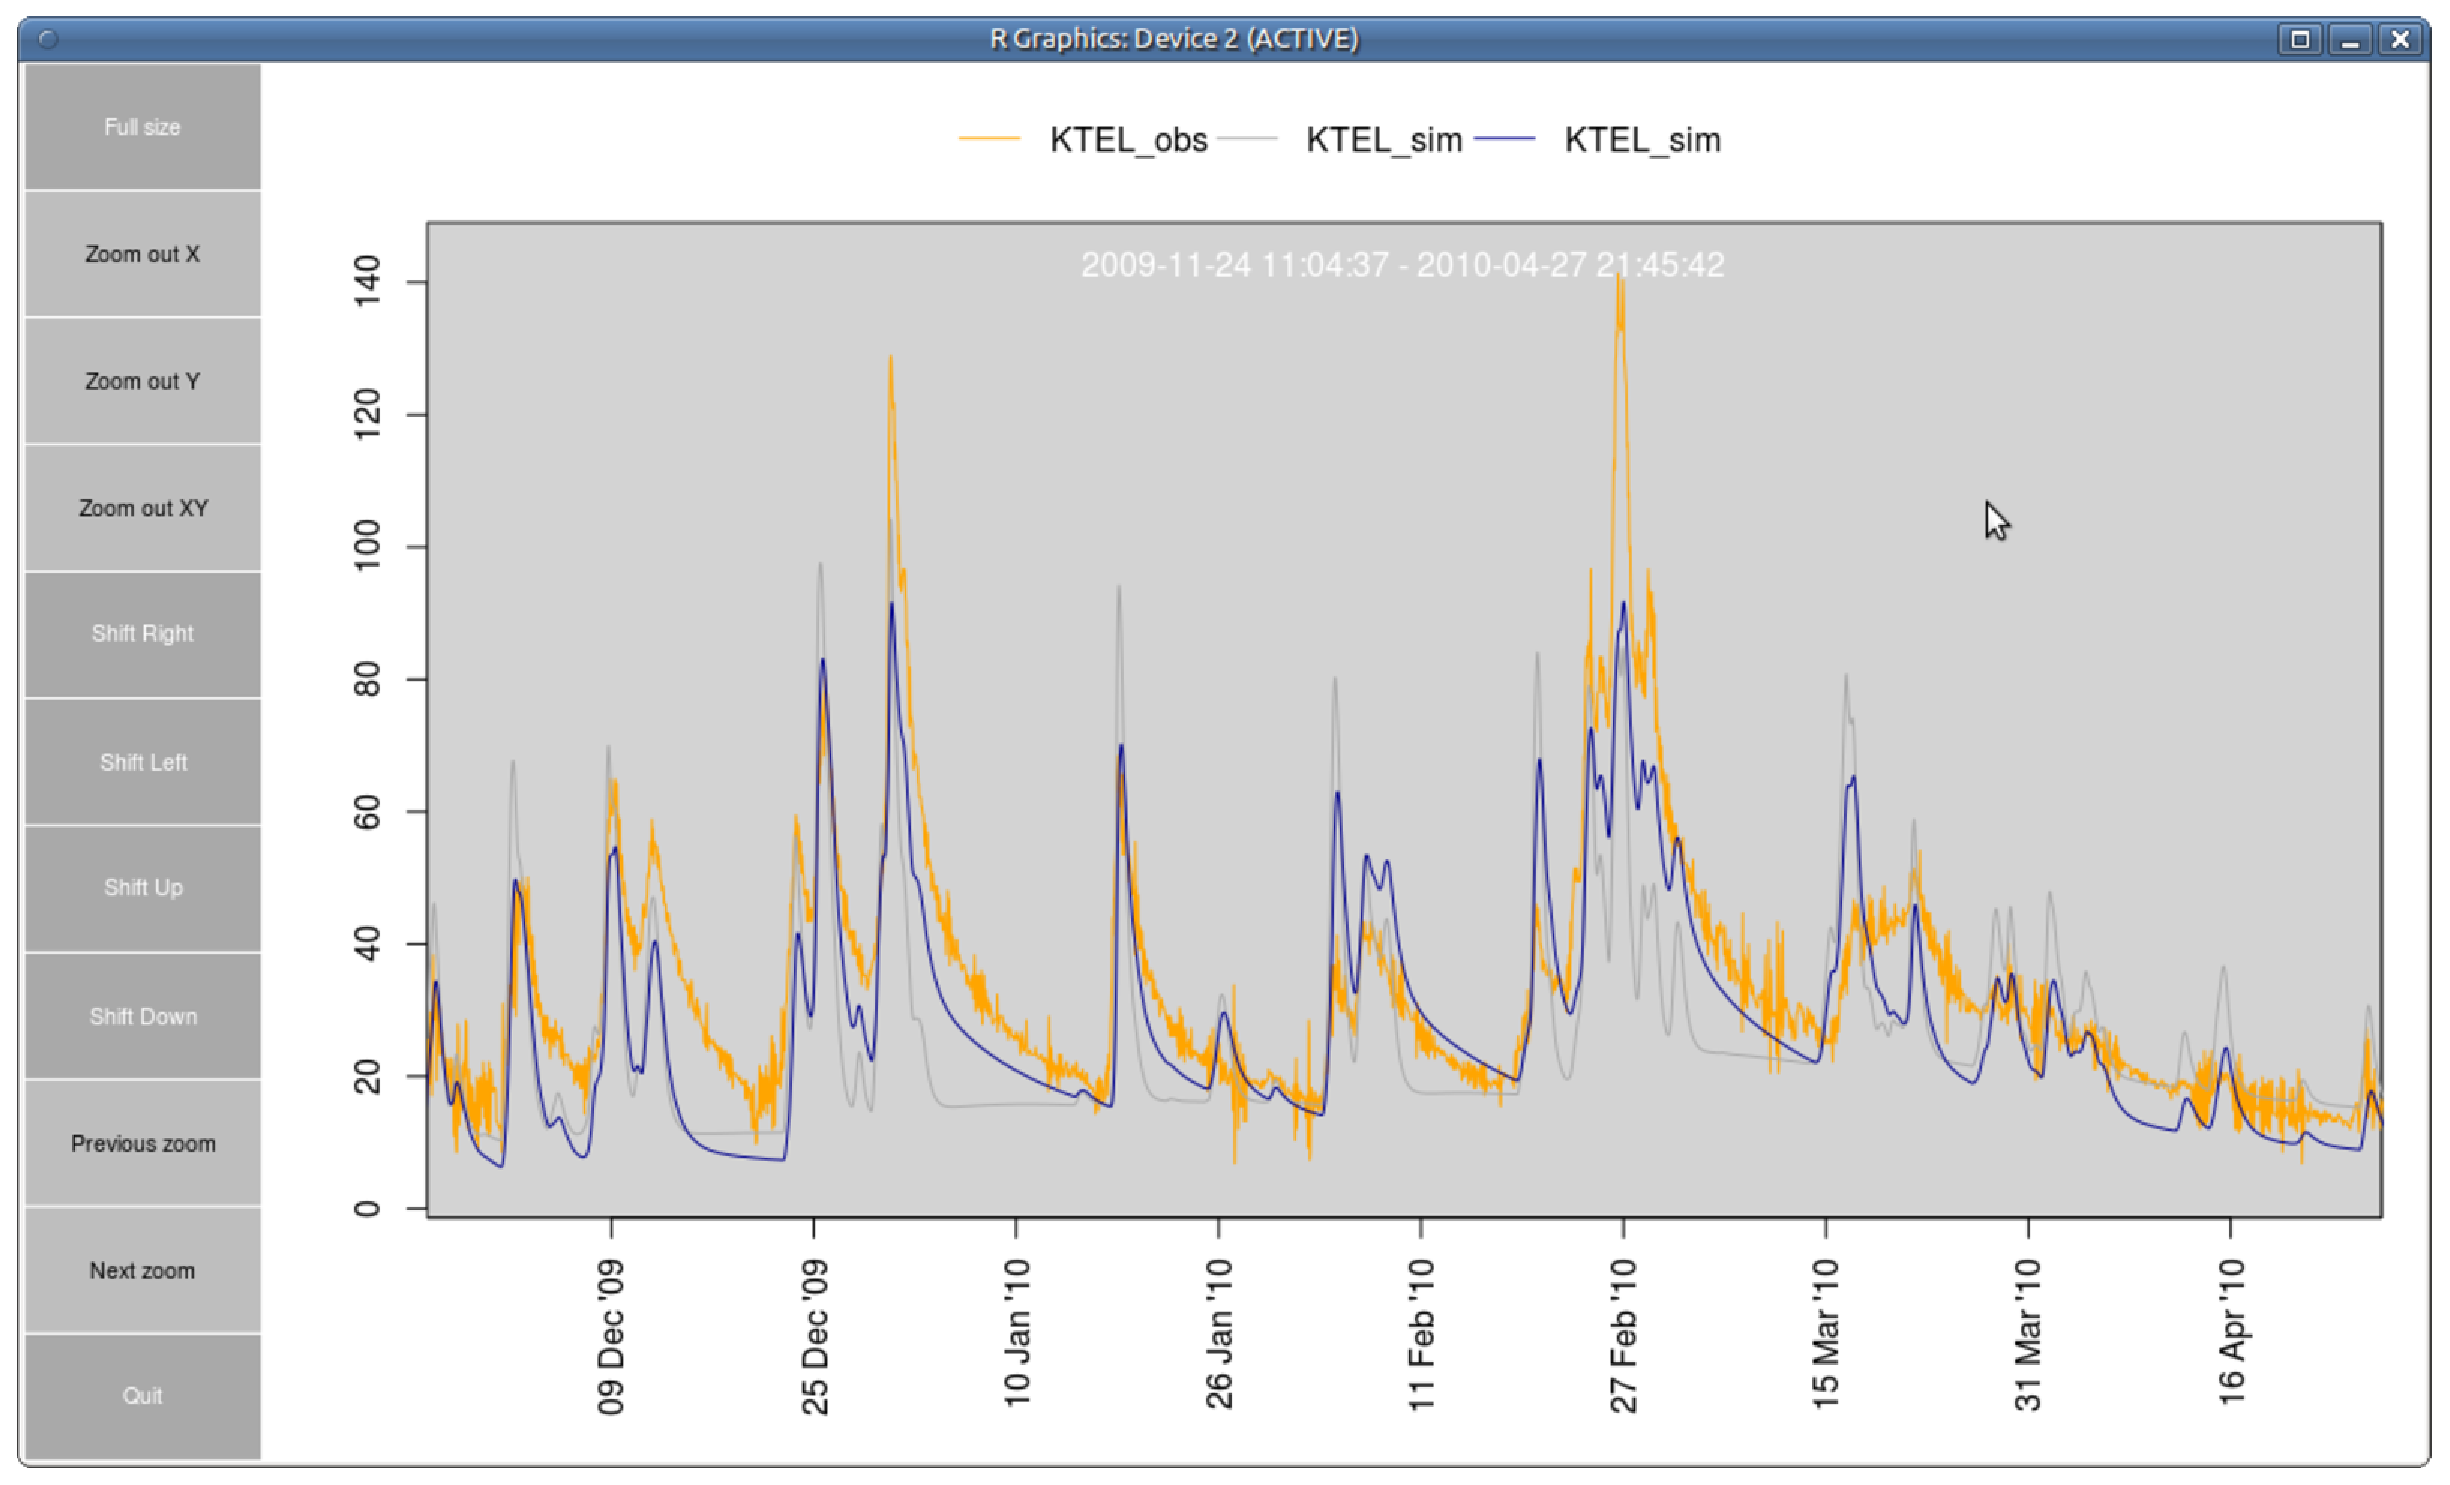
\includegraphics[width=0.9\textwidth]{\figdir/example.eps}
  \caption{Screen shot of a \software{tsplot} application. \label{fig:tsplot:example}}
\end{figure*}

%%%%%%%%%%%%%%%%%%%%%%%%%%%%%%%%%%%%%%%%%%%%%%%%%%%%%%%%%%%%%%%%%%%%%%%%%%%%%%%%
%%%%%%%%%%%%%%%%%%%%%%%%%%%%%%%%%%%%%%%%%%%%%%%%%%%%%%%%%%%%%%%%%%%%%%%%%%%%%%%%
%%%%%%%%%%%%%%%%%%%%%%%%%%%%%%%%%%%%%%%%%%%%%%%%%%%%%%%%%%%%%%%%%%%%%%%%%%%%%%%%
\section{Required software} \label{sec:tsplot:software}
\software{tsplot} is implemented as an R script. Thus, to use it, a current version of R must be installed. See \citet{Echse-Install-Doc} for information on how to install R. In order to invoke \software{tsplot} via a bash shell script under Windows, MSYS is required \citep[see][]{Echse-Install-Doc}.

%%%%%%%%%%%%%%%%%%%%%%%%%%%%%%%%%%%%%%%%%%%%%%%%%%%%%%%%%%%%%%%%%%%%%%%%%%%%%%%%
%%%%%%%%%%%%%%%%%%%%%%%%%%%%%%%%%%%%%%%%%%%%%%%%%%%%%%%%%%%%%%%%%%%%%%%%%%%%%%%%
%%%%%%%%%%%%%%%%%%%%%%%%%%%%%%%%%%%%%%%%%%%%%%%%%%%%%%%%%%%%%%%%%%%%%%%%%%%%%%%%
\section{Instructions files} \label{sec:tsplot:instructions}

The source(s) of the data to be plotted with \software{tsplot} and the corresponding styles are defined in instructions files. For every individual plot, one needs to create such a file. At a first glance, this may seem inconvenient. However, putting the instructions into a file allows for re-drawing a particular plot with only a single mouse click. In modeling studies -- and in particular during model calibration, when the data change frequently -- this is of great advantage.

Instruction files are plain text files containing data in a tabular format. The columns must be separated by white spaces (one or more spaces of tab characters). Each line of the file (row in the table) defines a time series to be plotted.

The instructions file must contain a table header with a complete set of column names (in any order). The meaning of the columns is as follows:
\begin{columndef}
  \item [file] (\textit{string}) Name of a text file containing time series data in the format described in \secref{sec:tsplot:datafiles}. Absolute or relative paths can be used. On Windows systems, it is important that the forward slash (\verb!/!) is used to separate the names of directories, instead of the usual backslash (\verb!\!).
  \item [colname] (\textit{string}) Name of a column existing in the data file specified in \texttt{file}. The values in this column are taken as the y-values. If the data file has no header, \ie{} no column names, one has to supply the index of the column rather than a name. The smallest useful index is 2 (see \secref{sec:tsplot:datafiles}).
  \item [color] (\textit{string}) Name of an existing color in R (examples: \emph{red} or \emph{lightblue}). Call the function \texttt{colors()} from an R prompt to display a (lengthy) list of all pre-defined color names.
  \item [type] (\textit{string}) This defines the style used for plotting. Using 'p' (for points) and 'l' (for lines) is appropriate for instantaneous data. For regular time series, where the values represent averages (or sums) over a intervals of time, you should 'S' or 's', depending on whether the given times specify the begin ('s') or the end ('S') of an interval. The output time series produced by \software{echse} models use the latter convention, thus you should use 'S'. Note that using 'p' may slow down the creation of plots significantly if the time series contain many values. In such cases, use one of the other options as an alternative.
  \item [name] (\textit{string}) A name for the series to appear in the legend.
  \item [header] (\textit{logical}) Must be a logical value (TRUE or FALSE in uppercase letters). If TRUE, \software{tsplot} expects the data file to contain a header with column names.
  \item [comment] (\textit{string}) A single character to be treated as a comment character in the data file. Quite often, the hash character (\verb!#!) is used for this purpose.
  \item [nodata] (\textit{string}) The value used in the data file to indicate missing values. Typical examples include 'NA' or '-9999'. The corresponding rows of the data file are ignored when creating the plot.
  \item [factor] (\textit{numeric}) A factor to be applied to the data before plotting. A value other that 1 may be useful to re-scale data when plotting multiple series whose values are of different magnitude.
  \item [xcut] (\textit{logical}) Must be a logical value (TRUE or FALSE in uppercase letters). If TRUE, the x-axis is truncated to the range of times contained in the data file. When plotting multiple series, a value of TRUE should not appear in more than 1 row of the instructions file.
\end{columndef}

An example of an instructions file is given in \figref{fig:tsplot:instructions-example}. If you need to put comment lines in the instructions file, use a semicolon as the first character of the line. The line will then be ignored by \software{tsplot} (see example in \figref{fig:tsplot:instructions-example}).

\begin{figure*}
  \lstinputlisting[style=txt]{\figdir/instructions-example.txt}
  \caption[Example of a \software{tsplot} instructions file.]{Example of a \software{tsplot} instructions file to display two time series of observed and simulated values. \label{fig:tsplot:instructions-example}}
\end{figure*}

%%%%%%%%%%%%%%%%%%%%%%%%%%%%%%%%%%%%%%%%%%%%%%%%%%%%%%%%%%%%%%%%%%%%%%%%%%%%%%%%
%%%%%%%%%%%%%%%%%%%%%%%%%%%%%%%%%%%%%%%%%%%%%%%%%%%%%%%%%%%%%%%%%%%%%%%%%%%%%%%%
%%%%%%%%%%%%%%%%%%%%%%%%%%%%%%%%%%%%%%%%%%%%%%%%%%%%%%%%%%%%%%%%%%%%%%%%%%%%%%%%
\section{Expected format of data files} \label{sec:tsplot:datafiles}
The actual time series data must be stored in plain text files. These file(s) must be formatted as follows:
\begin{itemize}
  \item A tabular format is expected with columns separated by the tab character (ASCII code 9).
  \item Time information must be in the \emph{first} column of the file.
  \item Times must be encoded as stings in ISO 8601 format (YYYY-MM-DD hh:mm:ss) with date and time separated by a single blank. Alternatively, one can provide only the date using the format YYYY-MM-DD. If only the date is given, a time of 00:00:00 is implicitly assumed.
  \item The times in column 1 may be given in regular \emph{or} irregular intervals. They should be in increasing order.
  \item The file can optionally have a header line specifying column names. Such names should be valid names in R, \ie{} the first character must be a letter. More letters, digits, and/or underscores may follow.
\end{itemize}

An example of a properly formatted time series file is shown in \figref{fig:tsplot:tseries-example}.

\begin{figure}
  \lstinputlisting[style=txt]{\figdir/tseries-example.txt}
  \caption{Example of a time series file for use with \software{tsplot}. \label{fig:tsplot:tseries-example}}
\end{figure}

%%%%%%%%%%%%%%%%%%%%%%%%%%%%%%%%%%%%%%%%%%%%%%%%%%%%%%%%%%%%%%%%%%%%%%%%%%%%%%%%
%%%%%%%%%%%%%%%%%%%%%%%%%%%%%%%%%%%%%%%%%%%%%%%%%%%%%%%%%%%%%%%%%%%%%%%%%%%%%%%%
%%%%%%%%%%%%%%%%%%%%%%%%%%%%%%%%%%%%%%%%%%%%%%%%%%%%%%%%%%%%%%%%%%%%%%%%%%%%%%%%
\section{Invoking \software{tsplot}} \label{sec:tsplot:invoke}

\subsection{On Linux} \label{sec:tsplot:invoke-linux}

On Linux, one needs to execute the shell script \texttt{tsplot.sh} and supply the name of the instructions file as a command line argument.

\subsubsection*{Using the command line}
Assuming that an instructions file \texttt{myplot.txt} exists in your home directory, a call from the command line might look as follows:

\begin{lstlisting}[style=shell]
  ./tsplot.sh /home/myname/myplot.txt
\end{lstlisting}

To use this, however, one first needs to navigate to the directory of \software{tsplot}, where the \texttt{tsplot.sh} resides. This is rather inconvenient. To be able to call \software{tsplot} from \emph{any} directory, you could do one of the following:

\begin{itemize}
  \item Move all files related to \software{tsplot} to a directory listed in the 'PATH' environment variable.
  \item Alternatively, add the path of the directory with the \software{tsplot} sources to the \verb!PATH! environment variable. See \citet{Echse-Install-Doc} for details.
  \item Alternatively, put a script in one of the directories already contained in the \verb!PATH! variable and let this script call \texttt{tsplot.sh}. In that case, you need to make sure that command line arguments are passed on.
\end{itemize}

\subsubsection*{Using the file browser's context menu}
In Ubuntu, Nautilus Actions provide the most convenient way to process an instructions file with \software{tsplot}. After defining a new action, you can simply process an instructions file from the Nautilus file browser's context menu. Thus, only two clicks with the right and left mouse buttons are necessary. See the documentation of Nautilus Actions for more info.

\subsection{On Windows} \label{sec:tsplot:invoke-windows}

On Windows, one needs to execute the batch file \texttt{tsplot.bat} and supply the name of the instructions file as a command line argument.

Assuming that an instructions file \verb!c:\temp\myplot.txt! exists, a call from the command line might look as follows:

\begin{lstlisting}[style=shell]
  tsplot.bat c:\temp\myplot.txt
\end{lstlisting}

To use this, however, one first needs to navigate to the directory of \software{tsplot}, where the \texttt{tsplot.bat} resides. To be able to call \software{tsplot} from \emph{any} directory, you could do one of the following:

\begin{itemize}
  \item Move all files related to \software{tsplot} to a directory listed in the \verb!path! environment variable.
  \item Alternatively, add the path of the directory with the \software{tsplot} sources to the \verb!path! environment variable. See \citet{Echse-Install-Doc} for details.
\end{itemize}

\subsubsection*{Using the file browser's context menu}
There are basically two ways:
\begin{itemize}
  \item Invent a new file extension for your instruction files (example: '.iii'). Create a new custom file type with that extension. Then configure the default 'open' action for the file type so that \texttt{tsplot.bat} is called with the file name as an argument. Thus, the 'open' action should read like \verb!some-path\tsplot.bat "%1"!.
  \item Alternatively, one can modify the 'open' action of any file type by editing the Windows registry. This is recommended for experienced users only and will not be described here.
\end{itemize}


%%%%%%%%%%%%%%%%%%%%%%%%%%%%%%%%%%%%%%%%%%%%%%%%%%%%%%%%%%
%%%%%%%%%%%%%%%%%%%%% LISTS %%%%%%%%%%%%%%%%%%%%%%%%%%%%%%
%%%%%%%%%%%%%%%%%%%%%%%%%%%%%%%%%%%%%%%%%%%%%%%%%%%%%%%%%%
\clearpage
\fancyhead[LE,RO]{\bfseries\thepage}
\fancyhead[RE]{\bfseries List of figures}
\fancyhead[LO]{\bfseries List of figures}
\addcontentsline{toc}{chapter}{List of figures}
\listoffigures

\clearpage
\fancyhead[LE,RO]{\bfseries\thepage}
\fancyhead[RE]{\bfseries List of tables}
\fancyhead[LO]{\bfseries List of tables}
\addcontentsline{toc}{chapter}{List of tables}
\listoftables

%%%%%%%%%%%%%%%%%%%%%%%%%%%%%%%%%%%%%%%%%%%%%%%%%%%%%%%%%%
%%%%%%%%%%%%%%%%%%%%% BIBLIOGRAPHY %%%%%%%%%%%%%%%%%%%%%%%
%%%%%%%%%%%%%%%%%%%%%%%%%%%%%%%%%%%%%%%%%%%%%%%%%%%%%%%%%%
\clearpage
\fancyhead[LE,RO]{\bfseries\thepage}
\fancyhead[RE]{\bfseries Bibliography}
\fancyhead[LO]{}
\addcontentsline{toc}{chapter}{Bibliography}
\bibliographystyle{../../_common/elsarticle-harv}
\bibliography{/home/dkneis/literature/jabref/bib_hydrologicalModeling,/home/dkneis/literature/jabref/bib_diplomaAndDiss}

%%%%%%%%%%%%%%%%%%%%%%%%%%%%%%%%%%%%%%%%%%%%%%%%%%%%%%%%%%
%%%%%%%%%%%%%%%%%%%%% THE APPENDIX %%%%%%%%%%%%%%%%%%%%%%%
%%%%%%%%%%%%%%%%%%%%%%%%%%%%%%%%%%%%%%%%%%%%%%%%%%%%%%%%%%

%\chaptermark{A}
%\clearpage
%\fancyhead[LE,RO]{\bfseries\thepage}
%\fancyhead[RE]{\bfseries Appendix}
%\fancyhead[LO]{}
%\addcontentsline{toc}{chapter}{Appendix}
%\appendix
%\input{appendix/bla/bla.tex}

%%%%%%%%%%%%%%%%%%%%%%%%%%%%%%%%%%%%%%%%%%%%%%%%%%%%%%%%%%
%%%%%%%%%%%%%%%%%%%%% THE INDEX %%%%%%%%%%%%%%%%%%%%%%%%%%
%%%%%%%%%%%%%%%%%%%%%%%%%%%%%%%%%%%%%%%%%%%%%%%%%%%%%%%%%%

\clearpage
\fancyhead[LE,RO]{\bfseries\thepage}
\fancyhead[RE]{\bfseries Index}
\fancyhead[LO]{}
\addcontentsline{toc}{chapter}{Index}
\printindex

\end{document}
